% Options for packages loaded elsewhere
\PassOptionsToPackage{unicode}{hyperref}
\PassOptionsToPackage{hyphens}{url}
%
\documentclass[
]{book}
\usepackage{lmodern}
\usepackage{amssymb,amsmath}
\usepackage{ifxetex,ifluatex}
\ifnum 0\ifxetex 1\fi\ifluatex 1\fi=0 % if pdftex
  \usepackage[T1]{fontenc}
  \usepackage[utf8]{inputenc}
  \usepackage{textcomp} % provide euro and other symbols
\else % if luatex or xetex
  \usepackage{unicode-math}
  \defaultfontfeatures{Scale=MatchLowercase}
  \defaultfontfeatures[\rmfamily]{Ligatures=TeX,Scale=1}
\fi
% Use upquote if available, for straight quotes in verbatim environments
\IfFileExists{upquote.sty}{\usepackage{upquote}}{}
\IfFileExists{microtype.sty}{% use microtype if available
  \usepackage[]{microtype}
  \UseMicrotypeSet[protrusion]{basicmath} % disable protrusion for tt fonts
}{}
\makeatletter
\@ifundefined{KOMAClassName}{% if non-KOMA class
  \IfFileExists{parskip.sty}{%
    \usepackage{parskip}
  }{% else
    \setlength{\parindent}{0pt}
    \setlength{\parskip}{6pt plus 2pt minus 1pt}}
}{% if KOMA class
  \KOMAoptions{parskip=half}}
\makeatother
\usepackage{xcolor}
\IfFileExists{xurl.sty}{\usepackage{xurl}}{} % add URL line breaks if available
\IfFileExists{bookmark.sty}{\usepackage{bookmark}}{\usepackage{hyperref}}
\hypersetup{
  pdftitle={Indicadores de reportes},
  pdfauthor={Observatorio Venezolano de Violencia},
  hidelinks,
  pdfcreator={LaTeX via pandoc}}
\urlstyle{same} % disable monospaced font for URLs
\usepackage{longtable,booktabs}
% Correct order of tables after \paragraph or \subparagraph
\usepackage{etoolbox}
\makeatletter
\patchcmd\longtable{\par}{\if@noskipsec\mbox{}\fi\par}{}{}
\makeatother
% Allow footnotes in longtable head/foot
\IfFileExists{footnotehyper.sty}{\usepackage{footnotehyper}}{\usepackage{footnote}}
\makesavenoteenv{longtable}
\usepackage{graphicx,grffile}
\makeatletter
\def\maxwidth{\ifdim\Gin@nat@width>\linewidth\linewidth\else\Gin@nat@width\fi}
\def\maxheight{\ifdim\Gin@nat@height>\textheight\textheight\else\Gin@nat@height\fi}
\makeatother
% Scale images if necessary, so that they will not overflow the page
% margins by default, and it is still possible to overwrite the defaults
% using explicit options in \includegraphics[width, height, ...]{}
\setkeys{Gin}{width=\maxwidth,height=\maxheight,keepaspectratio}
% Set default figure placement to htbp
\makeatletter
\def\fps@figure{htbp}
\makeatother
\setlength{\emergencystretch}{3em} % prevent overfull lines
\providecommand{\tightlist}{%
  \setlength{\itemsep}{0pt}\setlength{\parskip}{0pt}}
\setcounter{secnumdepth}{5}
\usepackage{booktabs}
\usepackage[utf8]{inputenc}
\usepackage[spanish]{babel}
\usepackage{amsthm}
\makeatletter
\def\thm@space@setup{%
  \thm@preskip=8pt plus 2pt minus 4pt
  \thm@postskip=\thm@preskip
}
\makeatother
\usepackage[]{natbib}
\bibliographystyle{apalike}

\title{Indicadores de reportes}
\author{Observatorio Venezolano de Violencia}
\date{2021-10-03}

\begin{document}
\maketitle

{
\setcounter{tocdepth}{1}
\tableofcontents
}
\hypertarget{prefacio}{%
\chapter*{Prefacio}\label{prefacio}}
\addcontentsline{toc}{chapter}{Prefacio}

\hypertarget{introducciuxf3n}{%
\chapter{Introducción}\label{introducciuxf3n}}

\hypertarget{metodo}{%
\chapter{Metodología}\label{metodo}}

Adoptamos la Clasificación Internacional de Delitos con Fines Estadísticos (ICCS por sus siglas en inglés) para contar con un marco general que incluye conceptos, definiciones y principios sobre delitos convenidos intencionalmente. Este instrumento fue elaborado por la Oficina de las Naciones Unidas contra la Droga y el Delito (UNODC) y liberado en el 2015 \citep{UNODC2015}.

La ICCS proporciona un marco conceptual común para elaborar y comparar de forma sistemática datos estadísticos obtenidos en cualquiera de las etapas del proceso de justicia penal, así como en encuestas de victimización (ICCS, 2015; Pág. 7). La ICCS al ofrecer un marco general, sirve a nivel nacional para estructurar y organizar datos estadísticos que obedezcan a categorías analíticas y no jurídicas. El uso de conceptos y definiciones estandarizadas no sólo permite la recopilación, el análisis y la difusión sistemática de datos, también facilita el análisis del delito (Ibidem).

De las muchas razones para tomar esa decisión está que la función principal de los observatorios de prensa es recabar información para conformar una base estadística sobre la ocurrencia del delito interpersonal violento en las regiones del país y con ella analizar sus móviles, distribución y evolución. No está demás destacar el valor que tiene que haya sido el OVV la primera organización del país en adoptar el uso del ICCS para sistematizar sus datos sobre el delito violento en nuestro medio.

Es cierto que la información proporcionada por los medios que han asegurado los observatorios es en muchos casos insuficiente para cumplimentar satisfactoriamente el instrumento, pero el estudio de los conceptos, definiciones y principios del ICCS es un requisito indispensable para mejorar las capacidades de los observatorios en el llenado del instrumento de captura de datos.

La preocupación mayor sobre la falta de comparabilidad, que es real, aún con la estandarización que supone el uso de la ICCS, está en la variabilidad de las fuentes de información por medio de los cuales los observatorios regionales recopilan sus datos. Por un lado los medios informativos siguen políticas editoriales distintas y obedecen a intereses de diversa naturaleza y por otro los periodistas o las personas que sirven de informantes emplean diferentes aproximaciones y criterios en el reporte de los sucesos. Expresado en términos estadísticos, decimos que hay sesgos de selección y variabilidad no controlada en el tratamiento del dato por parte de los generadores de la información. Desde una perspectiva metodológica, el dato estadístico agregado que producen los observatorios como estimación del delito violento ocurrido en sus regiones está inseparablemente asociado, técnicamente diríamos confundido, con las particularidades del proceso de recopilación de datos.

La ICCS constituye un marco general y no se puede pretender que cubra lo particular del delito de todos los países. Podemos y debemos ampliar, siempre que sea necesario, los tipos delictuales no incluidos pero que ocurran con frecuencia en el país, claro está siendo coherentes con lo establecido en el marco general del ICCS.

\hypertarget{indicadores-de-medios}{%
\chapter{Indicadores de medios}\label{indicadores-de-medios}}

\begin{verbatim}
## Error: Must group by variables found in `.data`.
## * Column `numero_delito` is not found.
\end{verbatim}

\begin{enumerate}
\def\labelenumi{\alph{enumi}.}
\tightlist
\item
  Fecha de inicio de la recolección de datos en el período cubierto: \textbf{01 ene. 2021}
\item
  Fecha de finalización de la recolección de datos en el período cubierto: \textbf{30 jun. 2021}
\item
  Total de delitos en el período cubierto: \textbf{2083}
\item
  Número de medios de información consultados: \textbf{55}
\end{enumerate}

\hypertarget{indicadores-numuxe9ricos-buxe1sicos}{%
\chapter{Indicadores numéricos básicos}\label{indicadores-numuxe9ricos-buxe1sicos}}

\begin{enumerate}
\def\labelenumi{\alph{enumi}.}
\item
  Número total de eventos: \textbf{2551}
\item
  Número total de eventos de muertes por intervención policial: \textbf{465}
\item
  Número total de eventos de delitos: \textbf{2085}
\item
  Número total del delito de homicidio intencional: \textbf{594}
\item
  Número total de tentativa de homicidio intencional: \textbf{142}
\item
  Número total de los delitos restantes: \textbf{1815}
\item
  Número total de muertes por intervención policial: \textbf{\(\ge\) 612}
\item
  Número total de víctimas de delitos reportados: \textbf{\(\ge\) 2855}
\item
  Número total de víctimas de homicidio intencional: \textbf{\(\ge\) 699}
\item
  Número total de víctimas de tentativa de homicidio intencional: \textbf{\(\ge\) 214}
\end{enumerate}

\hypertarget{vuxedctimas-intervenciuxf3n-policial}{%
\chapter{Víctimas intervención policial}\label{vuxedctimas-intervenciuxf3n-policial}}

\hypertarget{edad-y-sexo-de-la-vuxedctima}{%
\section{Edad y sexo de la víctima}\label{edad-y-sexo-de-la-vuxedctima}}



\begin{figure}
\centering
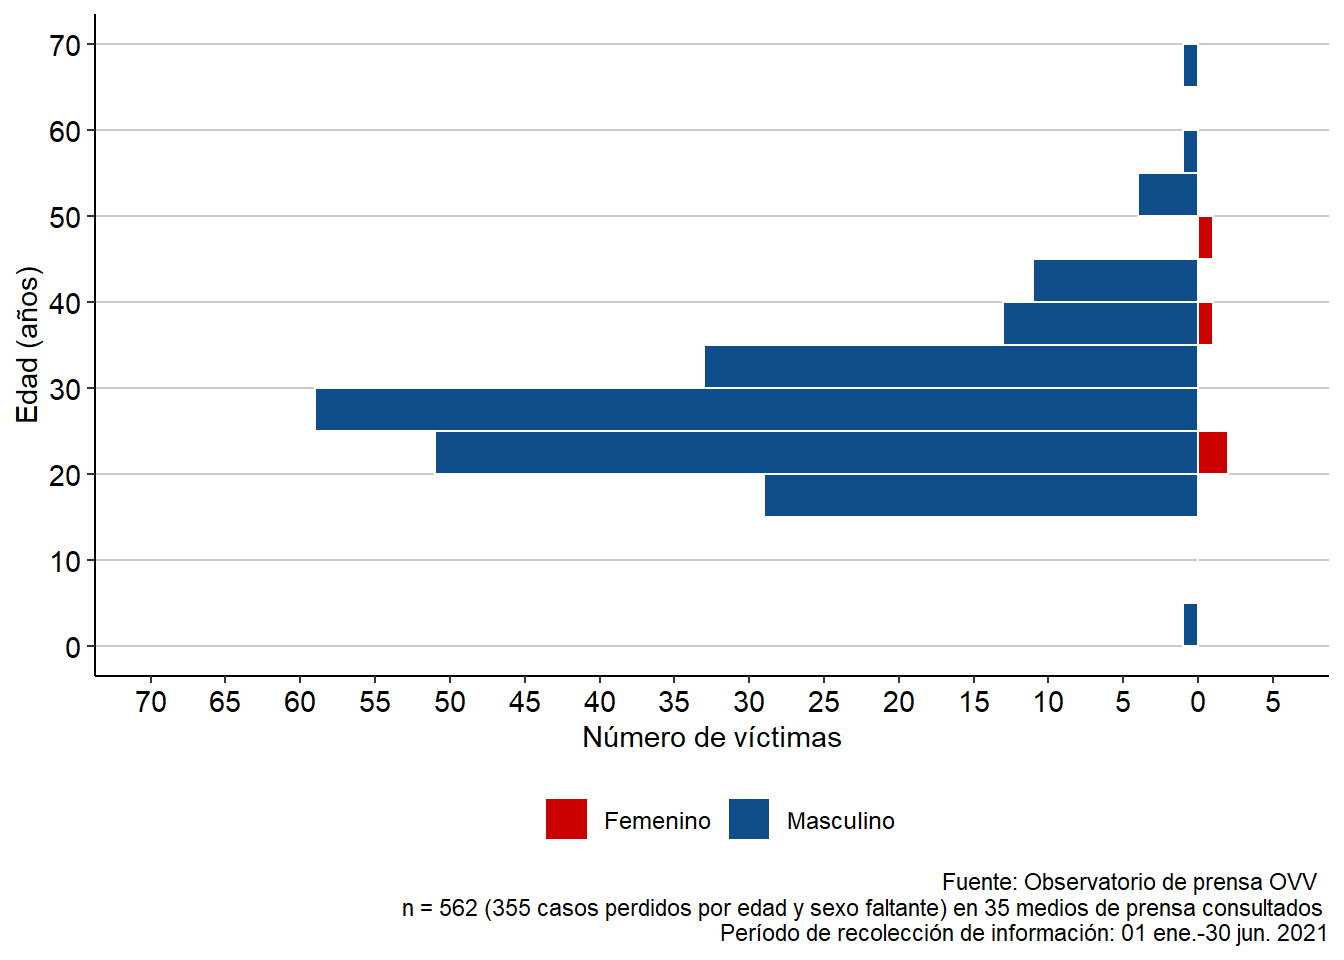
\includegraphics{bookdown-demo_files/figure-latex/victimasmiledadsexo-1.pdf}
\caption{\label{fig:victimasmiledadsexo}Número víctimas por intervención policial discriminados por edad y sexo.}
\end{figure}

\hypertarget{estado-conyugal-de-la-vuxedctima}{%
\section{Estado conyugal de la víctima}\label{estado-conyugal-de-la-vuxedctima}}



\begin{figure}
\centering
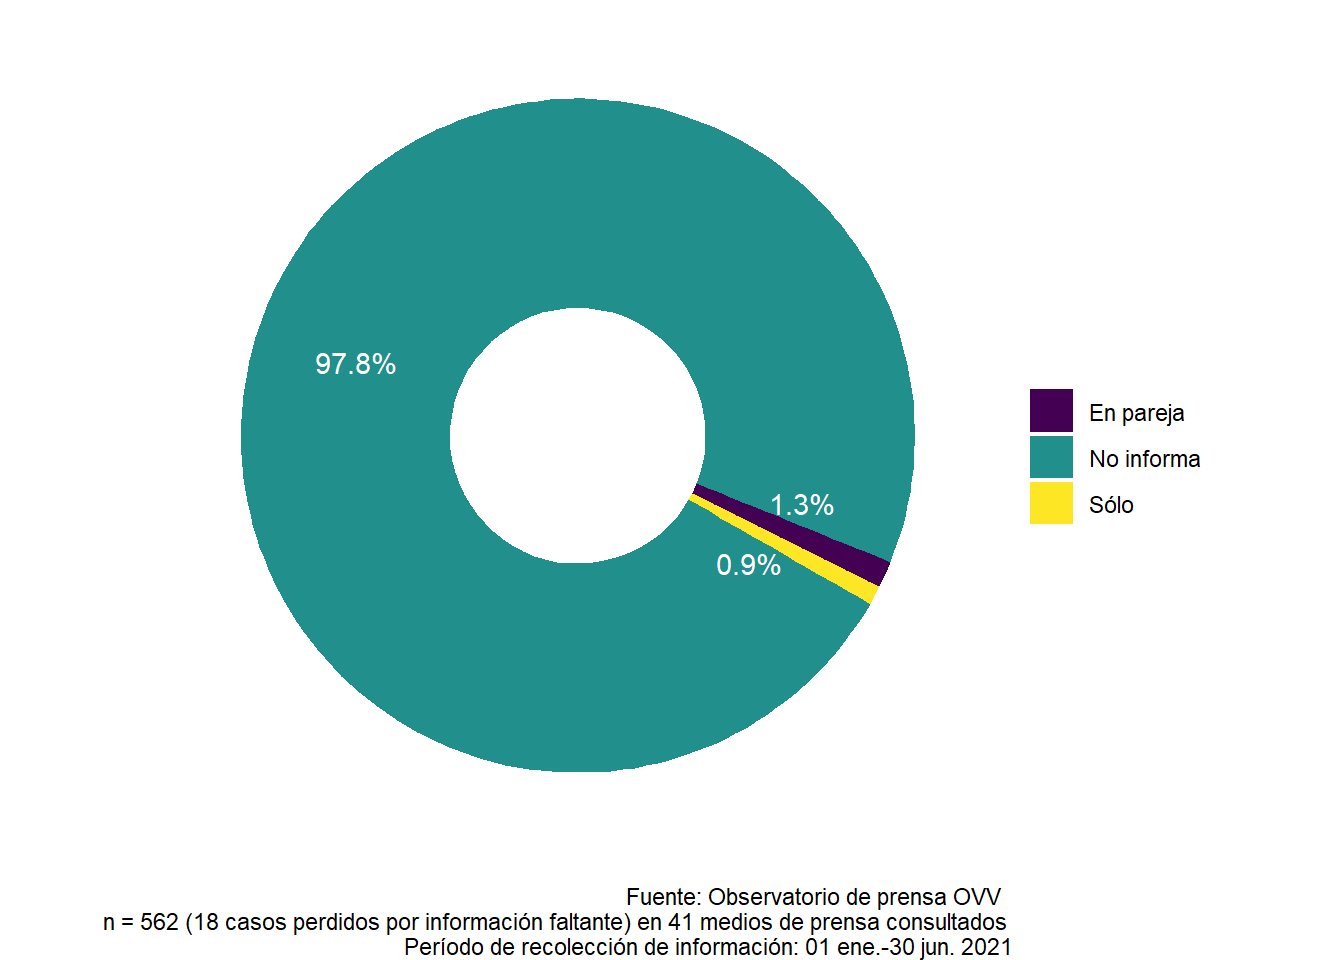
\includegraphics{bookdown-demo_files/figure-latex/victimasmilconyugal-1.pdf}
\caption{\label{fig:victimasmilconyugal}Estado conyugal de víctimas por intervención policial.}
\end{figure}

\hypertarget{condiciuxf3n-de-la-vuxedctima}{%
\section{Condición de la víctima}\label{condiciuxf3n-de-la-vuxedctima}}



\begin{figure}
\centering
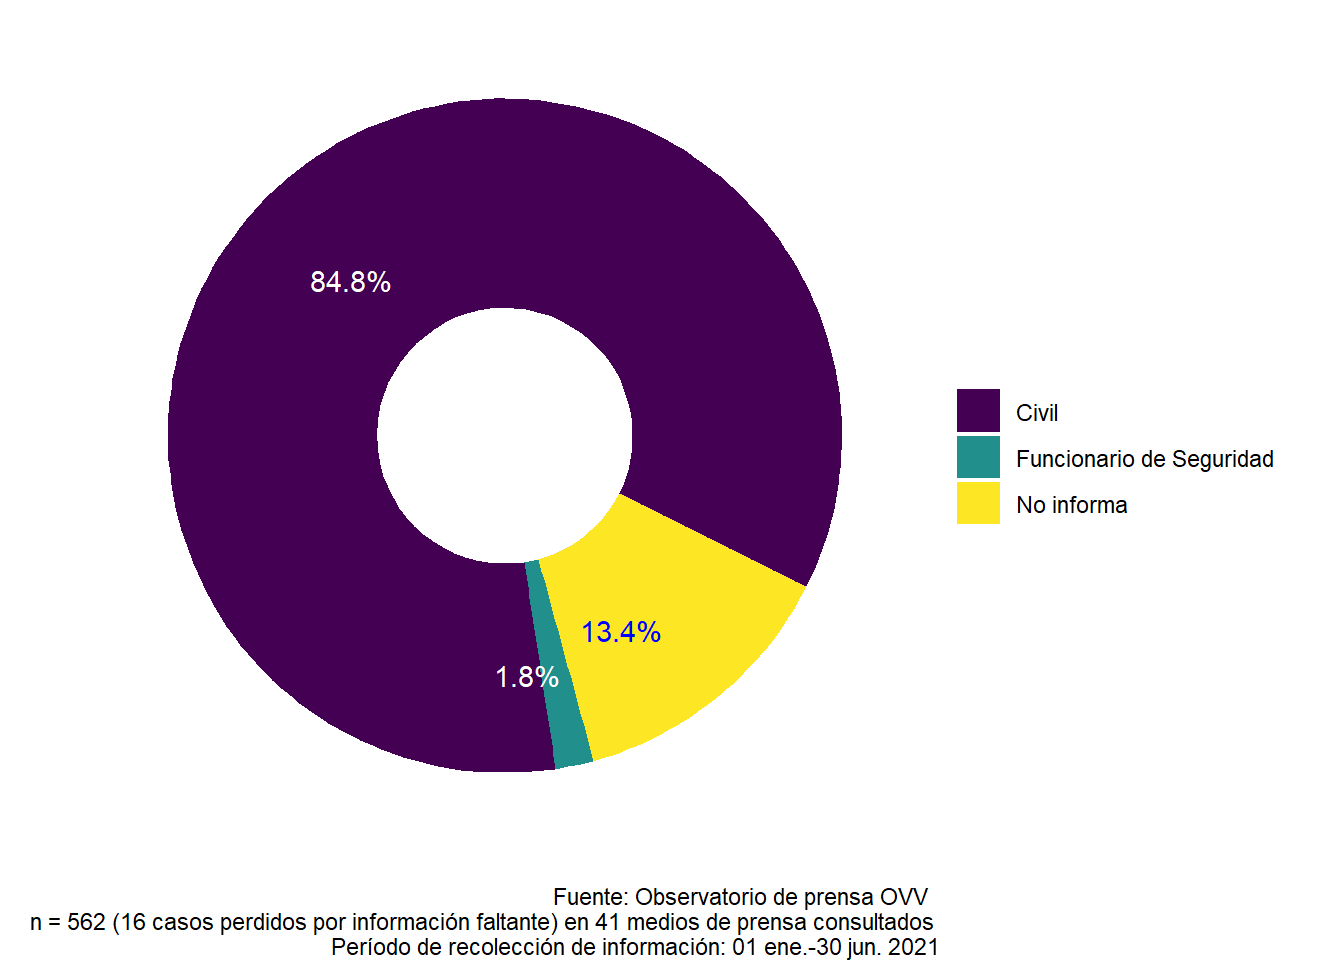
\includegraphics{bookdown-demo_files/figure-latex/victimasmilcondicion-1.pdf}
\caption{\label{fig:victimasmilcondicion}Proporción de víctimas por intervención policial que eran civiles o eran funcionarios de seguridad.}
\end{figure}

\hypertarget{la-vuxedctima-era-delincuente}{%
\section{¿La víctima era delincuente?}\label{la-vuxedctima-era-delincuente}}



\begin{figure}
\centering
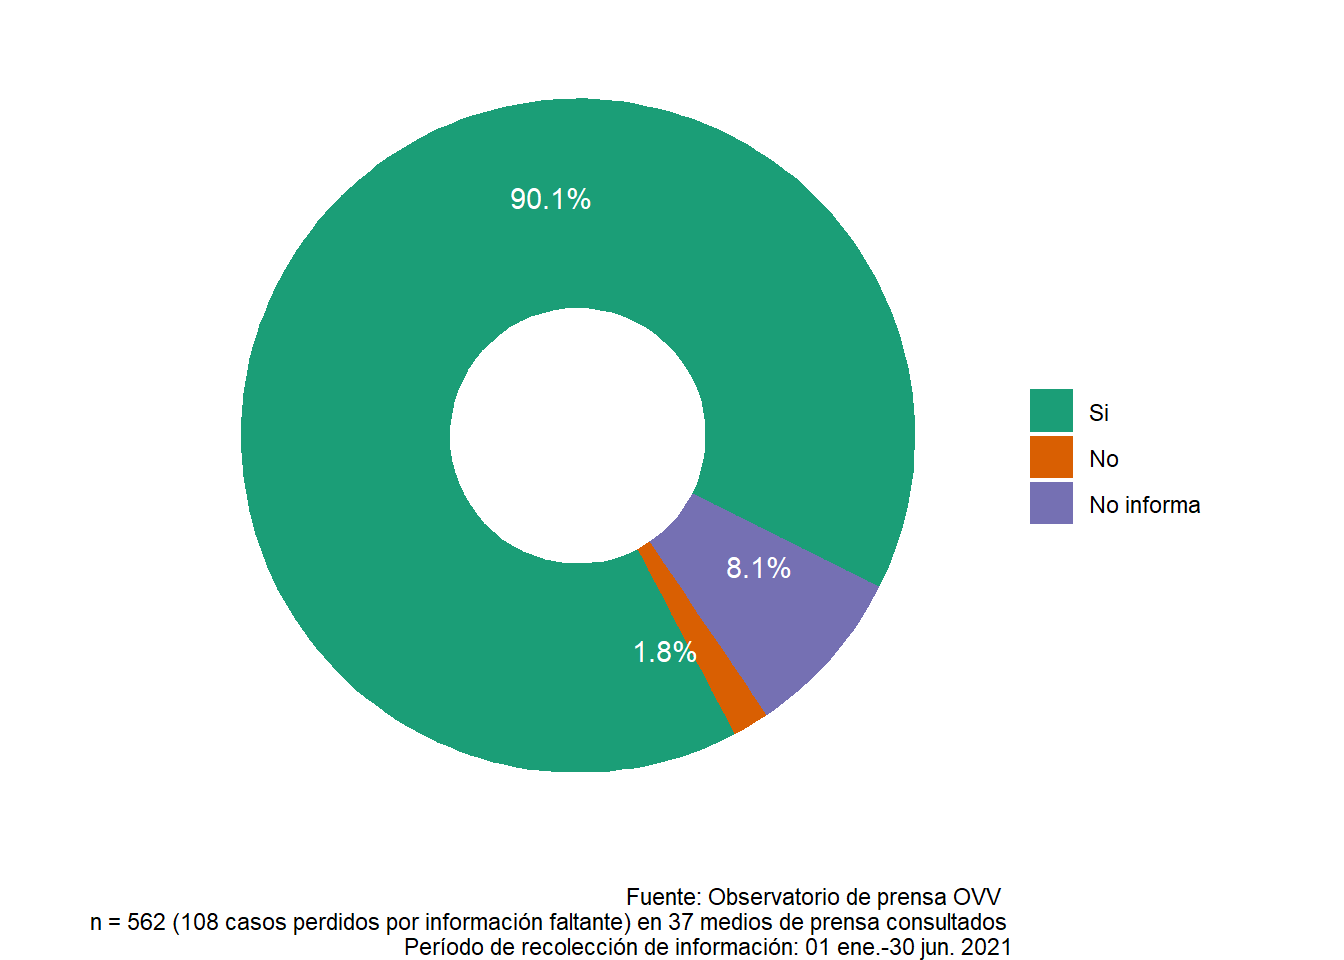
\includegraphics{bookdown-demo_files/figure-latex/victimasmildeligraf-1.pdf}
\caption{\label{fig:victimasmildeligraf}Proporción de víctimas que eran o no delincuentes.}
\end{figure}

\hypertarget{actividad-de-la-vuxedctima}{%
\section{Actividad de la víctima}\label{actividad-de-la-vuxedctima}}



\begin{figure}
\centering
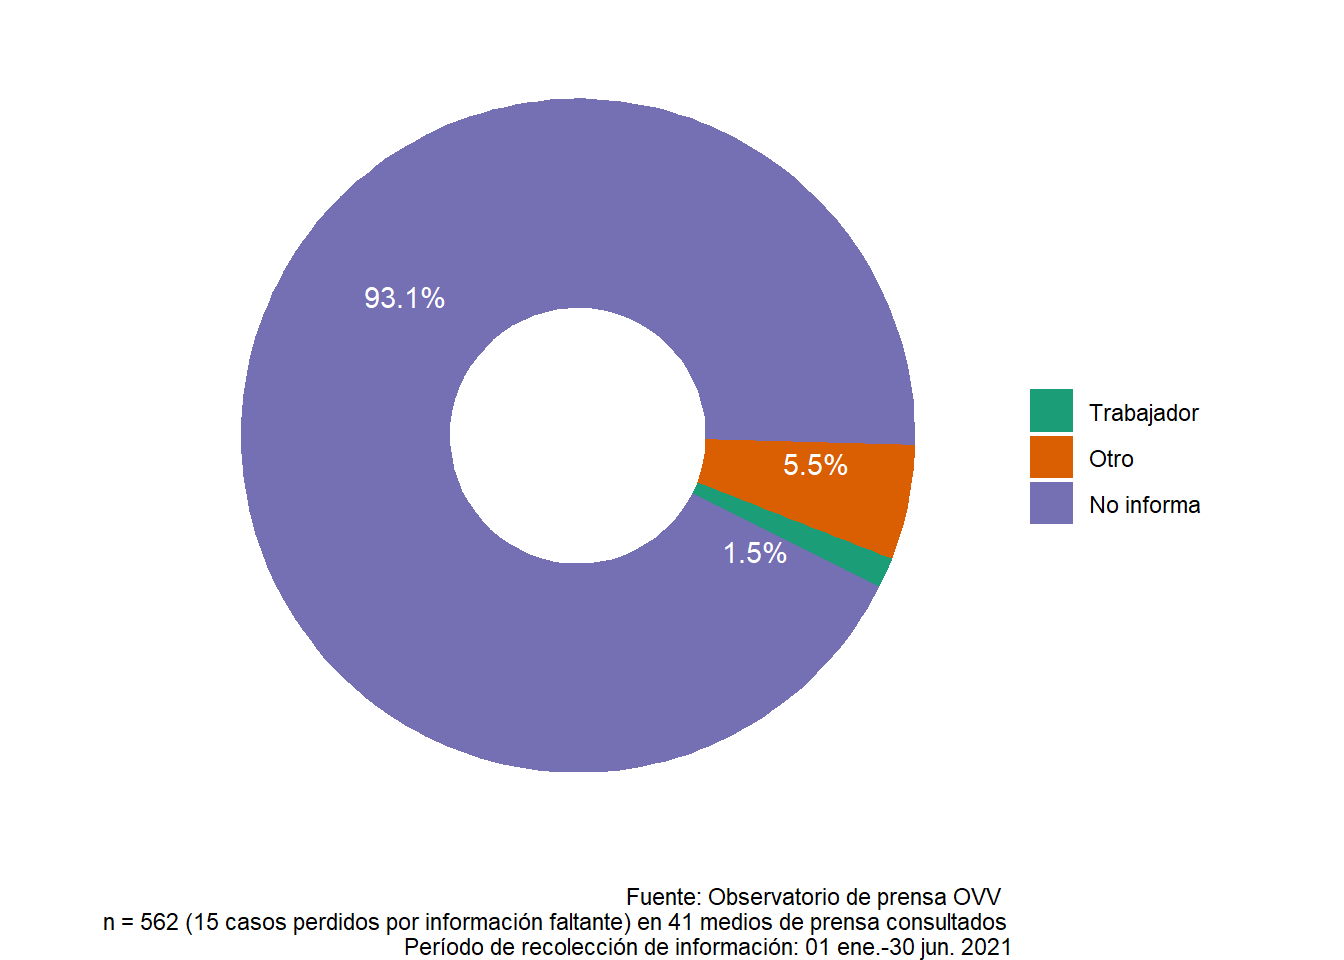
\includegraphics{bookdown-demo_files/figure-latex/victimasmilactividadgraf-1.pdf}
\caption{\label{fig:victimasmilactividadgraf}Proporción de víctimas que eran o no delincuentes.}
\end{figure}

\hypertarget{ocupaciuxf3n-de-la-vuxedctima}{%
\section{Ocupación de la víctima}\label{ocupaciuxf3n-de-la-vuxedctima}}



\begin{figure}
\centering
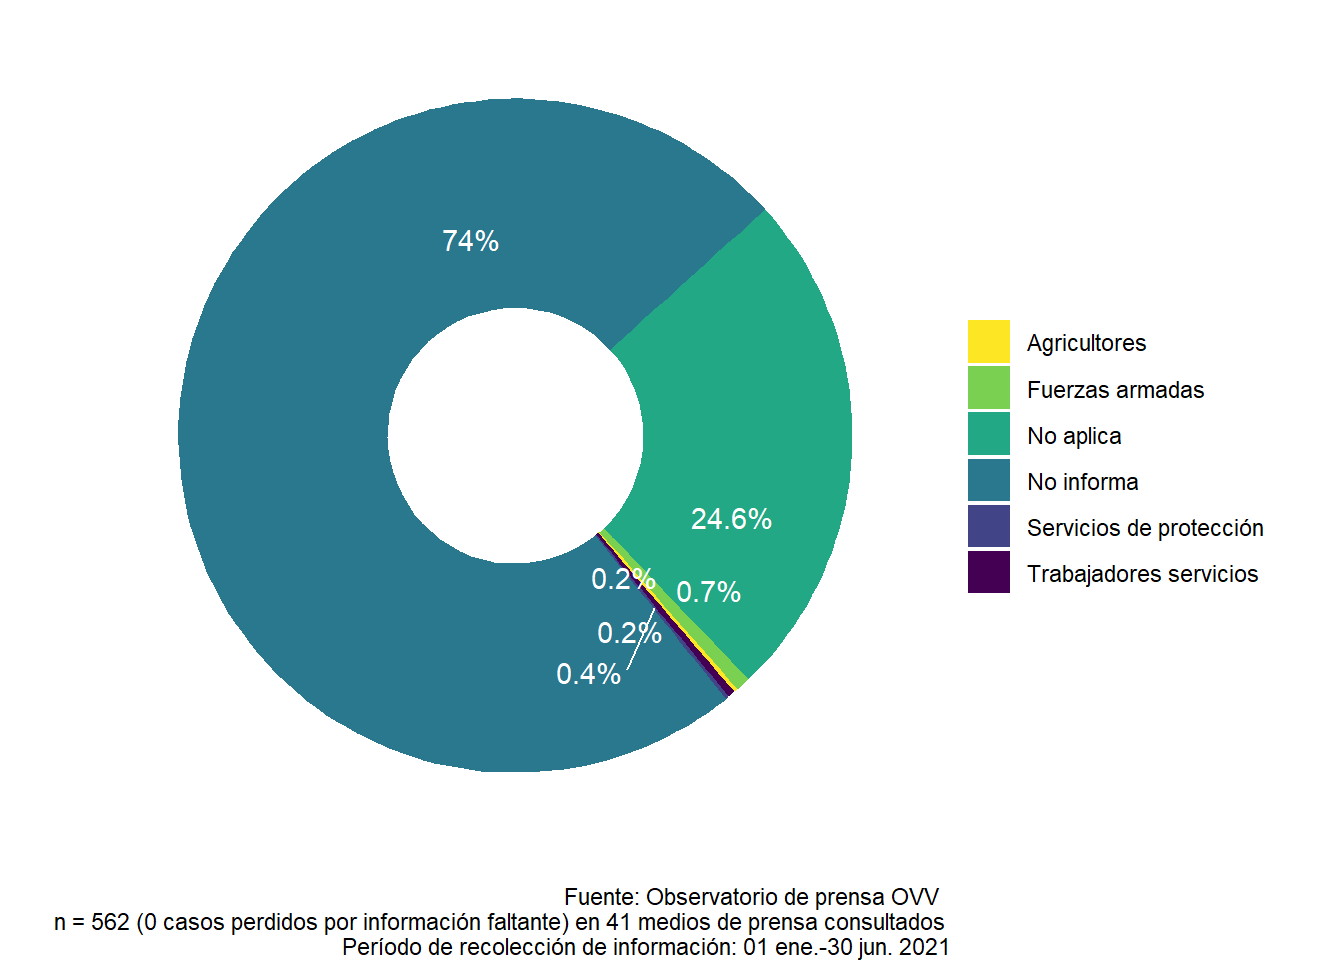
\includegraphics{bookdown-demo_files/figure-latex/victimasmilocupaciongraf-1.pdf}
\caption{\label{fig:victimasmilocupaciongraf}Proporción de víctimas por intervención policial según su ocupación.}
\end{figure}

\hypertarget{vuxedctimas-homicidio-intencional}{%
\chapter{Víctimas homicidio intencional}\label{vuxedctimas-homicidio-intencional}}

\hypertarget{edad-y-sexo-de-la-vuxedctima-1}{%
\section{Edad y sexo de la víctima}\label{edad-y-sexo-de-la-vuxedctima-1}}



\begin{figure}
\centering
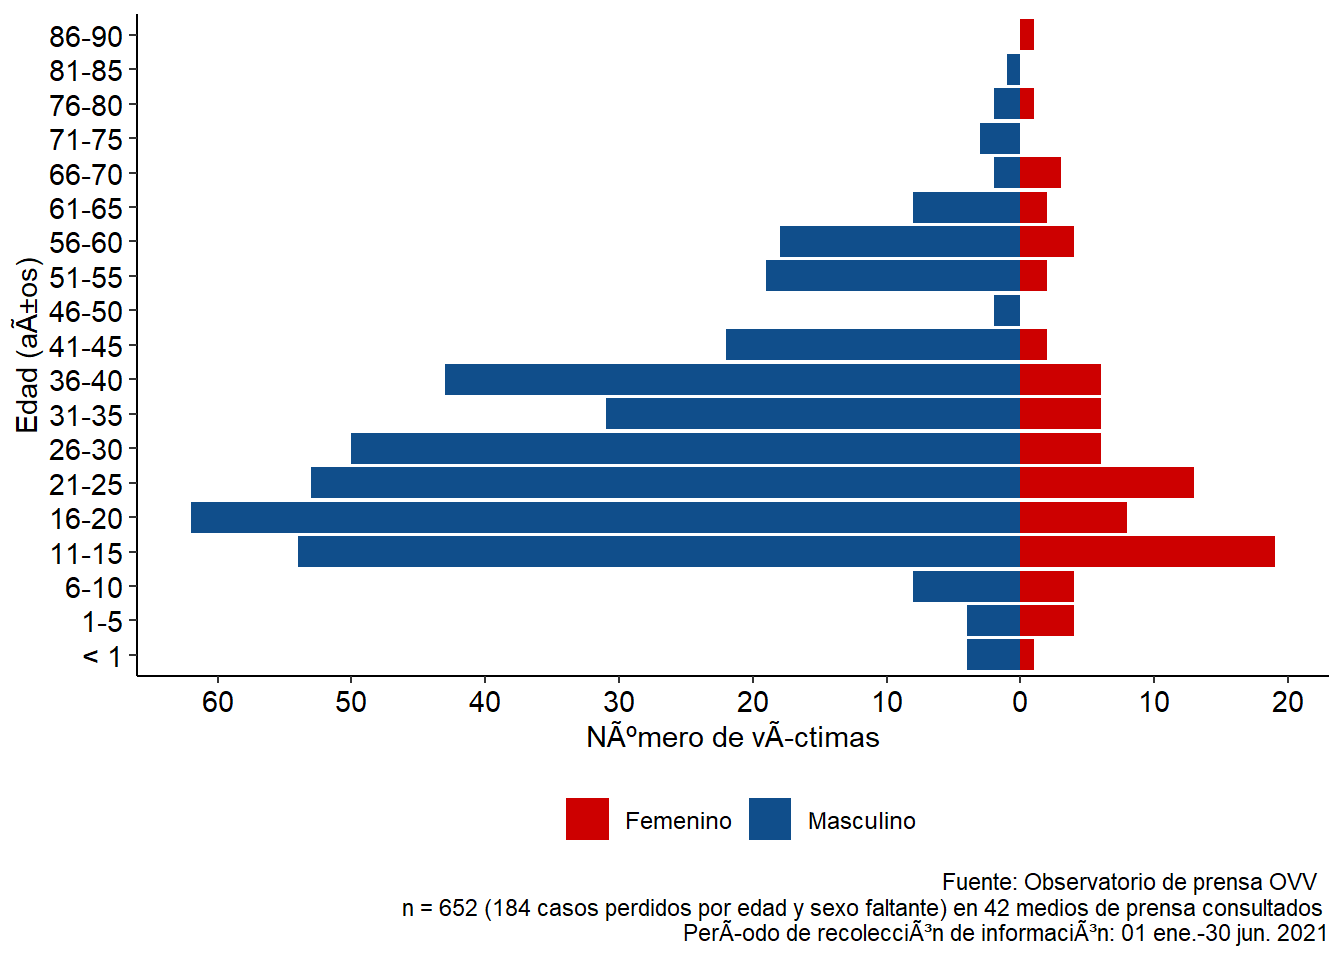
\includegraphics{bookdown-demo_files/figure-latex/victimasdelhiedadsexograf-1.pdf}
\caption{\label{fig:victimasdelhiedadsexograf}Número de víctimas por homicidio intencional discrimandos según edad y sexo.}
\end{figure}

\hypertarget{estado-conyugal-de-la-vuxedctima-1}{%
\section{Estado conyugal de la víctima}\label{estado-conyugal-de-la-vuxedctima-1}}



\begin{figure}
\centering
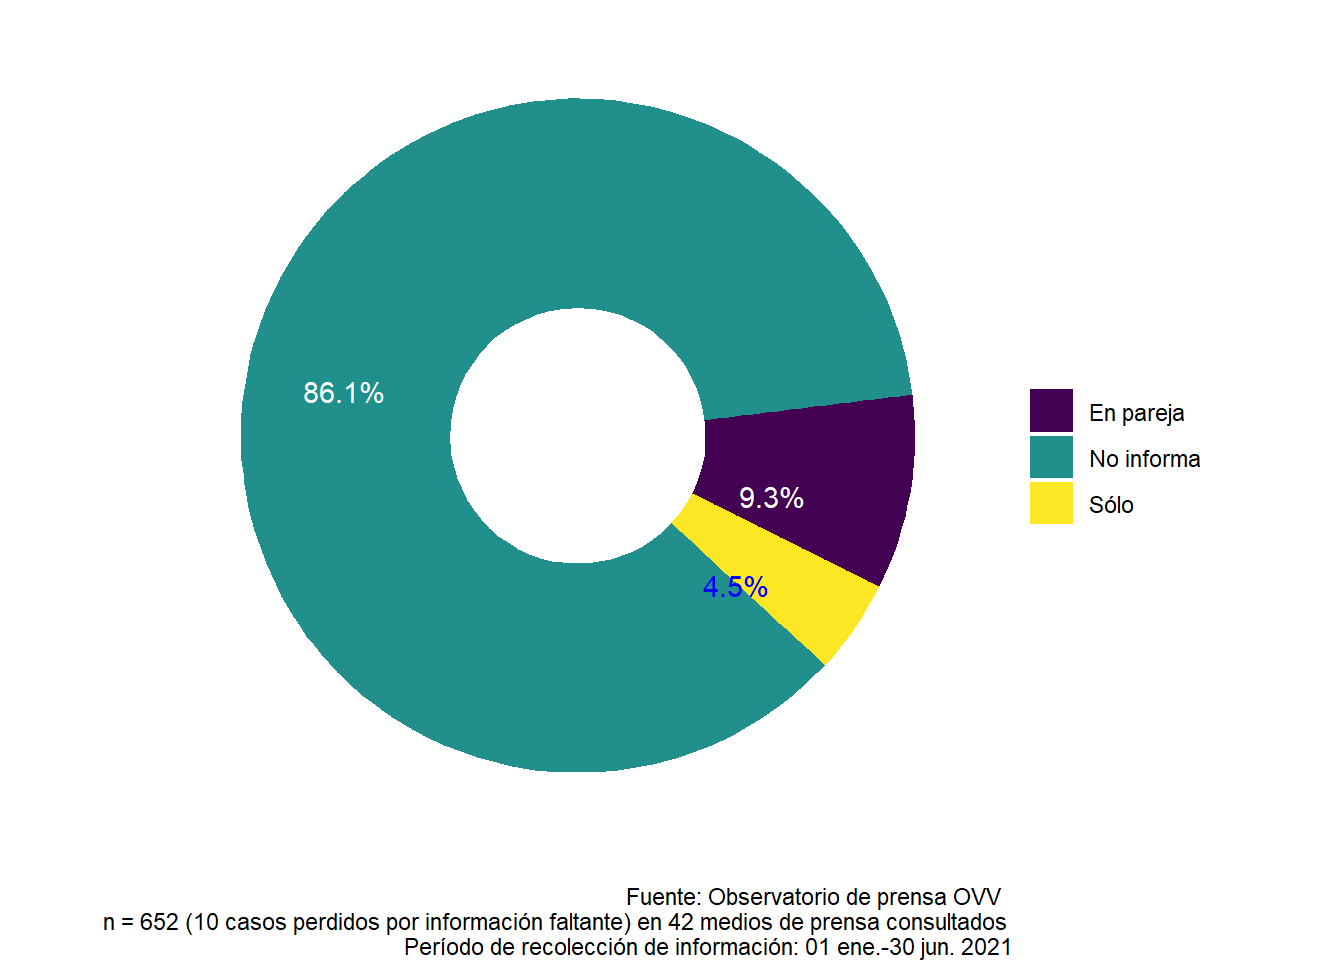
\includegraphics{bookdown-demo_files/figure-latex/victimasdelhiconyugalgraf-1.pdf}
\caption{\label{fig:victimasdelhiconyugalgraf}Número de víctimas por homicidio intencional discriminados según estado conyugal.}
\end{figure}

\hypertarget{polivictimizado}{%
\section{Polivictimizado}\label{polivictimizado}}



\begin{figure}
\centering
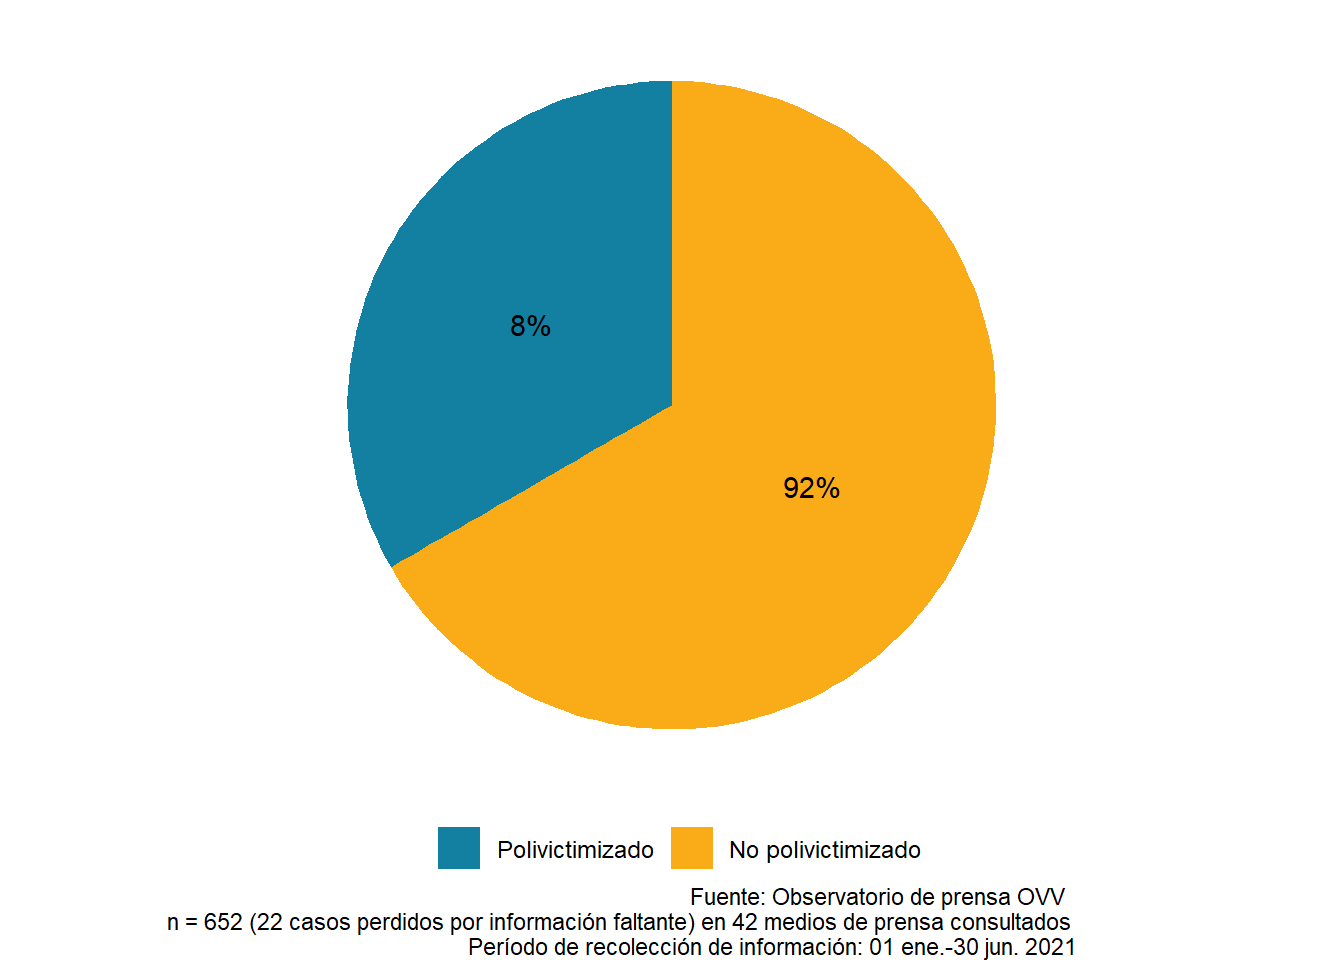
\includegraphics{bookdown-demo_files/figure-latex/victimasdelhipoligraf-1.pdf}
\caption{\label{fig:victimasdelhipoligraf}Número de víctimas por homicidio intencional discrimandos según condicion de polivictimización.}
\end{figure}

\hypertarget{condiciuxf3n-de-la-vuxedctima-1}{%
\section{Condición de la víctima}\label{condiciuxf3n-de-la-vuxedctima-1}}



\begin{figure}
\centering
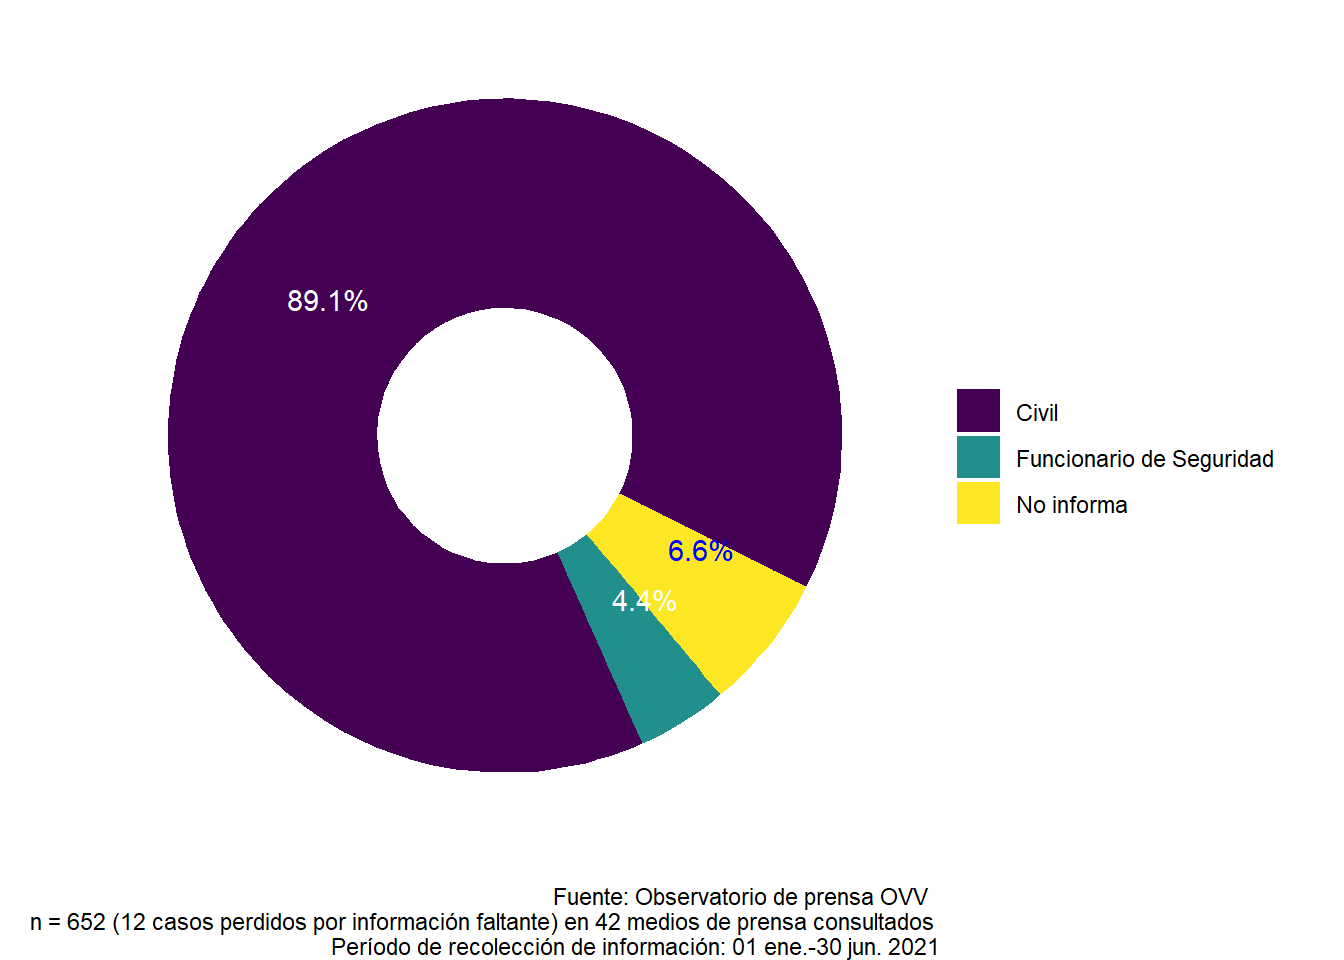
\includegraphics{bookdown-demo_files/figure-latex/victimasdelhicondigraf-1.pdf}
\caption{\label{fig:victimasdelhicondigraf}Número de víctimas por homicidio intencional discrimandos según condicion de civil o perteneciente a un cuerpo de seguridad.}
\end{figure}

\hypertarget{la-vuxedctima-era-delincuente-1}{%
\section{¿La víctima era delincuente?}\label{la-vuxedctima-era-delincuente-1}}



\begin{figure}
\centering
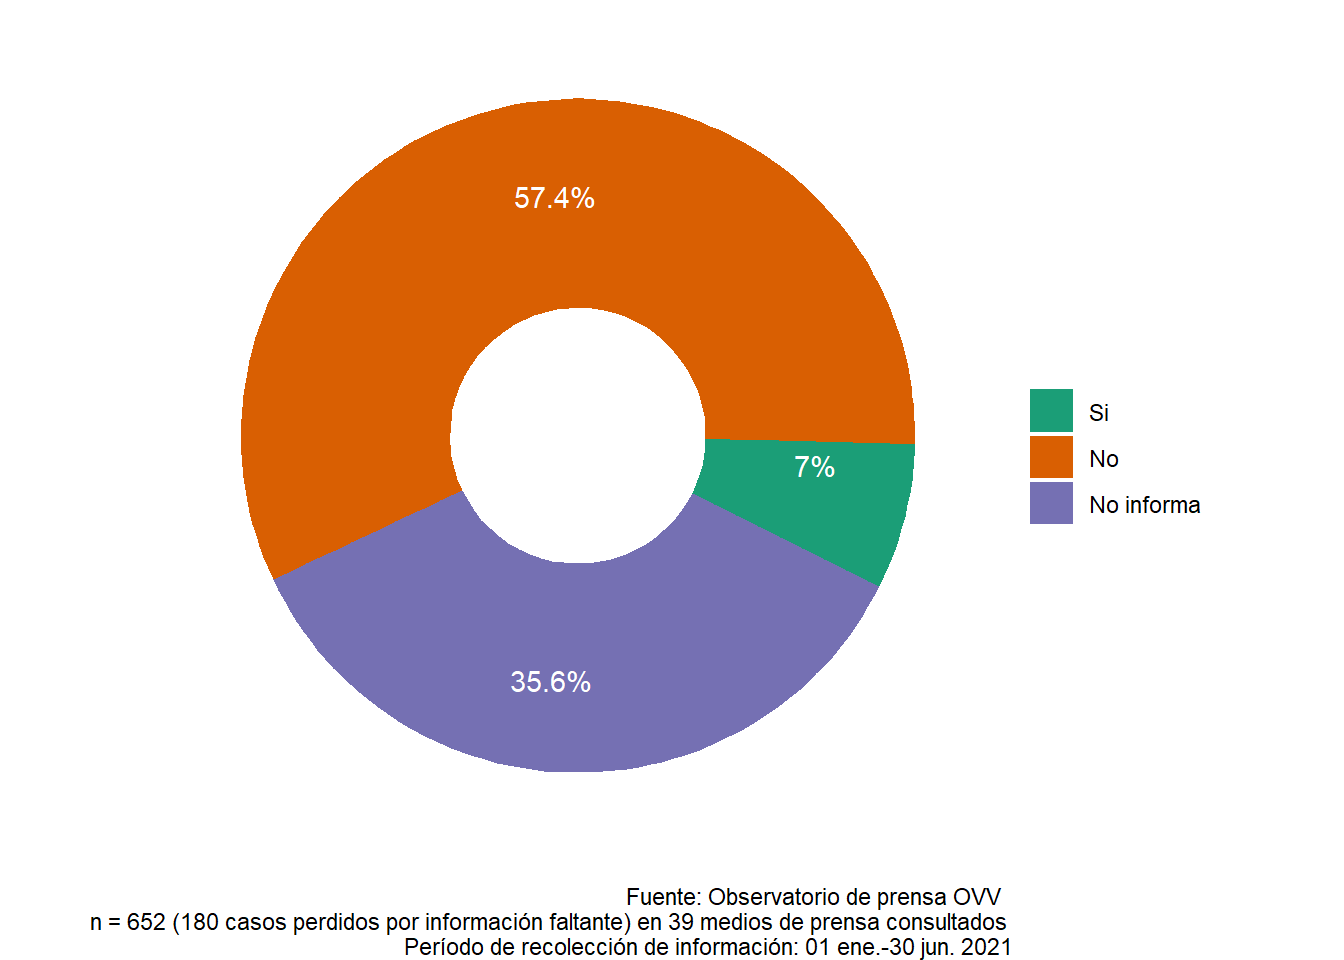
\includegraphics{bookdown-demo_files/figure-latex/victimasdelhivictideligraf-1.pdf}
\caption{\label{fig:victimasdelhivictideligraf}Número de víctimas por homicidio intencional discriminados según condición de ser o no delincuentes.}
\end{figure}

\hypertarget{actividad-de-la-vuxedctima-1}{%
\section{Actividad de la víctima}\label{actividad-de-la-vuxedctima-1}}



\begin{figure}
\centering
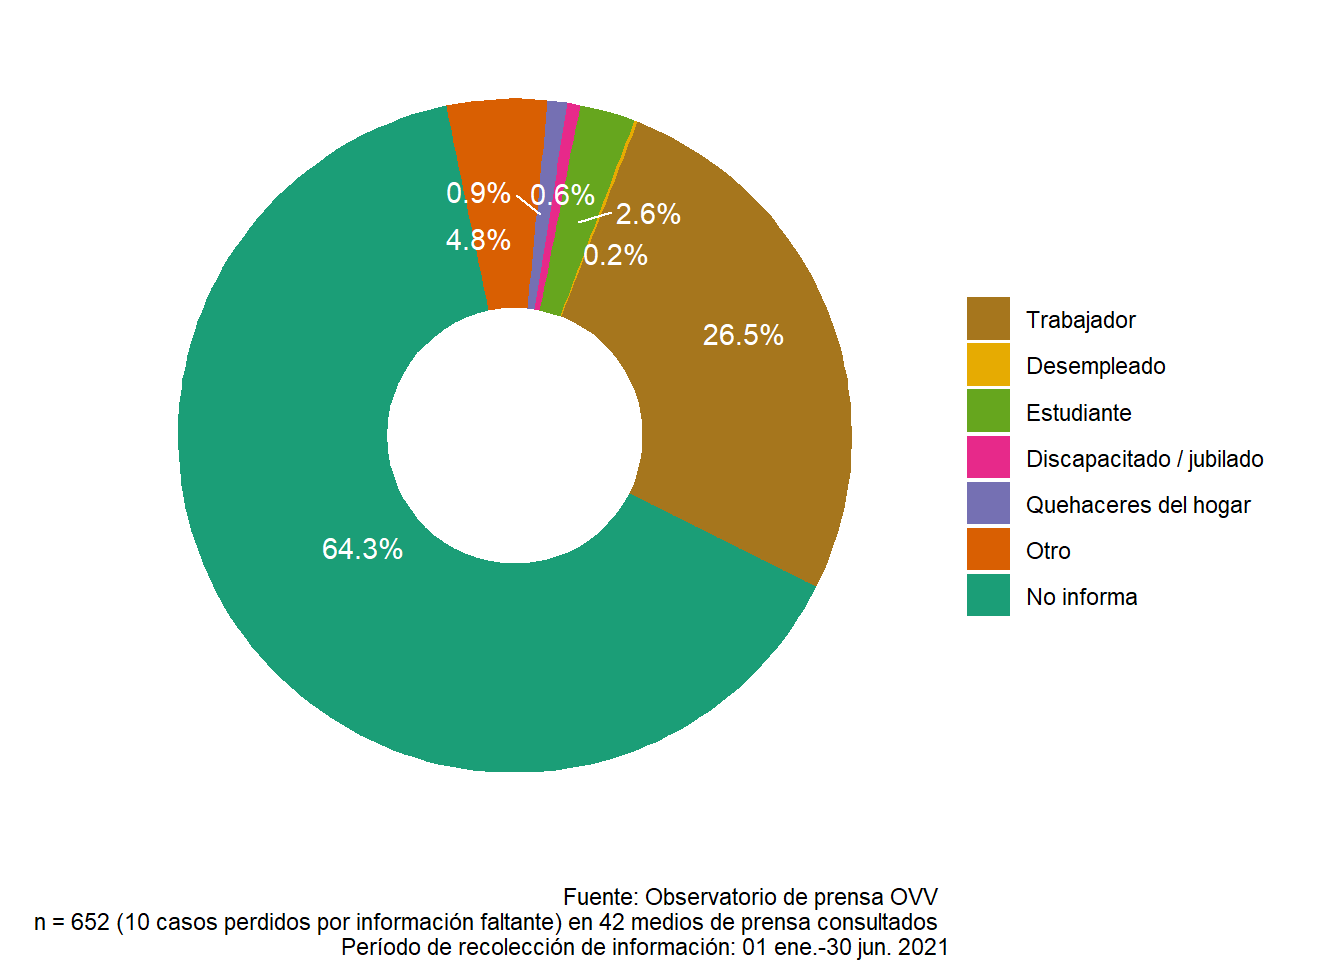
\includegraphics{bookdown-demo_files/figure-latex/victimasdelhiactividadgraf-1.pdf}
\caption{\label{fig:victimasdelhiactividadgraf}Número de víctimas por homicidio intencional discriminados según la actividad a la que se dedicaban.}
\end{figure}

\hypertarget{ocupaciuxf3n-de-la-vuxedctima-1}{%
\section{Ocupación de la víctima}\label{ocupaciuxf3n-de-la-vuxedctima-1}}

Tras una primera mirada a esta figura, rápidamente nos percatamos de lo difícil que resulta extraer y comprender la información. En parte, esta dificultad la podemos atribuir a las multiples opciones de ``ocupación'' en la que se subdividen los datos -como podemos apreciar en los elementos que integran la leyenda-. Otra posible razón es la paleta de colores, ya que la gradación no permite separar, visualmente, todas las opciones. Si bien es posible utilizar una paleta que delimite mejor entre las opciones, cuando son tantas, es preferible recurrir a otra representación para ayudar al lector.



\begin{figure}
\centering
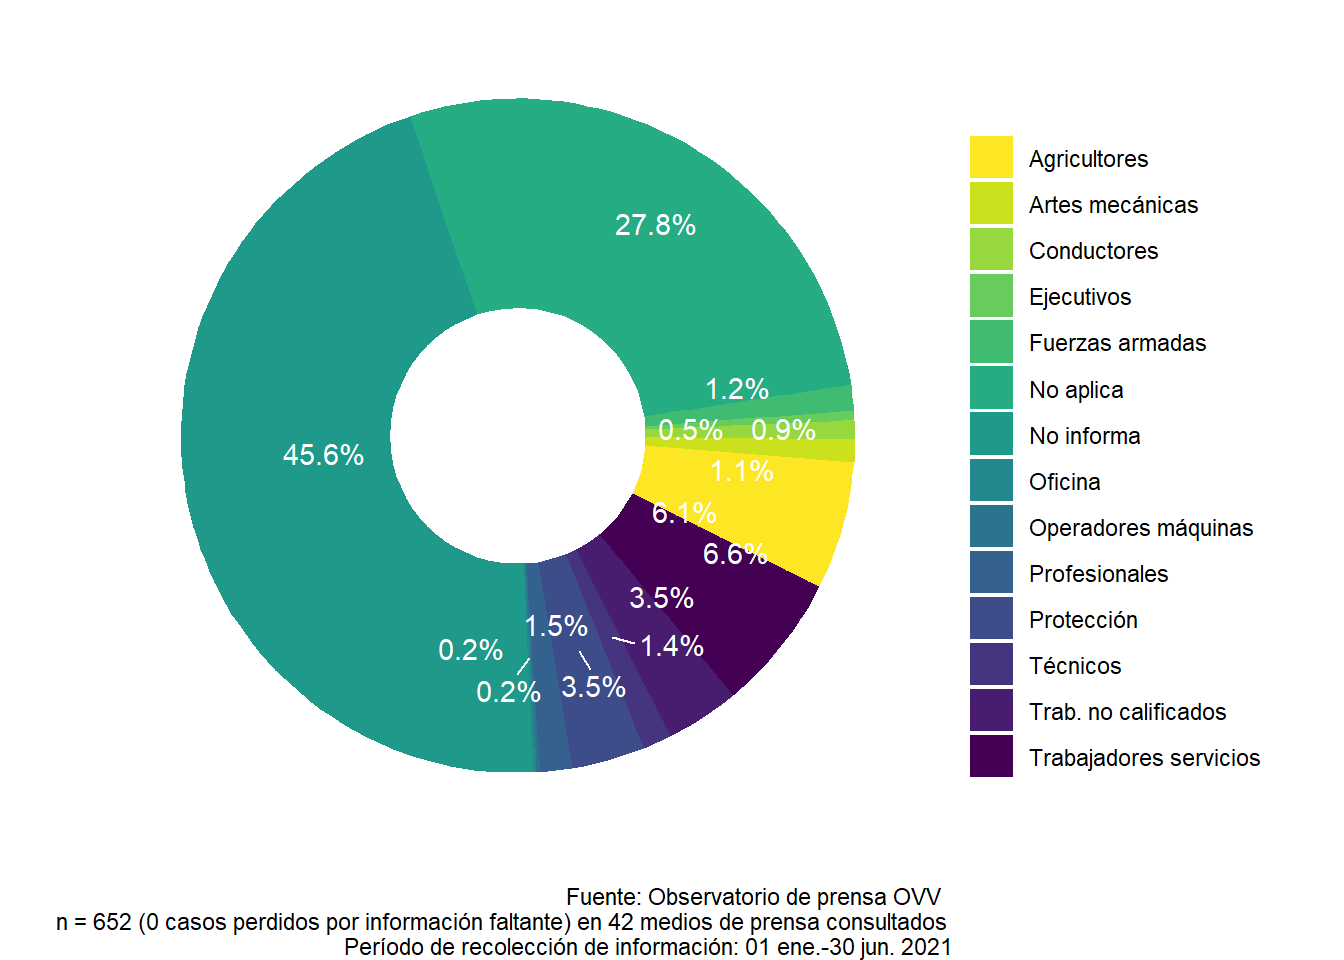
\includegraphics{bookdown-demo_files/figure-latex/victimasdelhiocupaciongraf-1.pdf}
\caption{\label{fig:victimasdelhiocupaciongraf}Número de víctimas por homicidio intencional discriminados según su ocupación.}
\end{figure}

En este sentido, una posible solución consistiría en sustituir la figura \ref{fig:victimasdelhiocupaciongraf} por una tabla. Este formato, sin lugar a dudas, ayudaría al usuario a extraer la información, en particular, con aquellas categorias que exhiben magnitudes bajas como se puede apreciar en la tabla \ref{tab:victimasdelhiocupaciontable}. Adicionalmente, la jerarquización según el orden de magnitud permite al lector tener una idea de la importancia de cada categoría con un mínimo esfuerzo



\begin{table}

\caption{\label{tab:victimasdelhiocupaciontable}\textbf{Número y proporción de víctimas por homicidio intencional discriminados por su ocupación. Período de recolección de información: 01 ene.-30 jun. 2021; n=652 (0 casos perdidos por información faltante) en 42 medios de prensa consultados.}}
\centering
\begin{tabular}[t]{lcr}
\toprule
Ocupación & Víctimas & Porcentaje\\
\midrule
No informa & 297 & 45.6\%\\
No aplica & 181 & 27.8\%\\
Trabajadores servicios & 43 & 6.6\%\\
Agricultores & 40 & 6.1\%\\
Protección & 23 & 3.5\%\\
\addlinespace
Trab. no calificados & 23 & 3.5\%\\
Profesionales & 10 & 1.5\%\\
Técnicos & 9 & 1.4\%\\
Fuerzas armadas & 8 & 1.2\%\\
Artes mecánicas & 7 & 1.1\%\\
\addlinespace
Conductores & 6 & 0.9\%\\
Ejecutivos & 3 & 0.5\%\\
Oficina & 1 & 0.2\%\\
Operadores máquinas & 1 & 0.2\%\\
\bottomrule
\end{tabular}
\end{table}

\hypertarget{eventos-intervenciuxf3n-policial}{%
\chapter{Eventos intervención policial}\label{eventos-intervenciuxf3n-policial}}

\hypertarget{cuerpos-de-seguridad}{%
\section{Cuerpos de seguridad}\label{cuerpos-de-seguridad}}



\begin{figure}
\centering
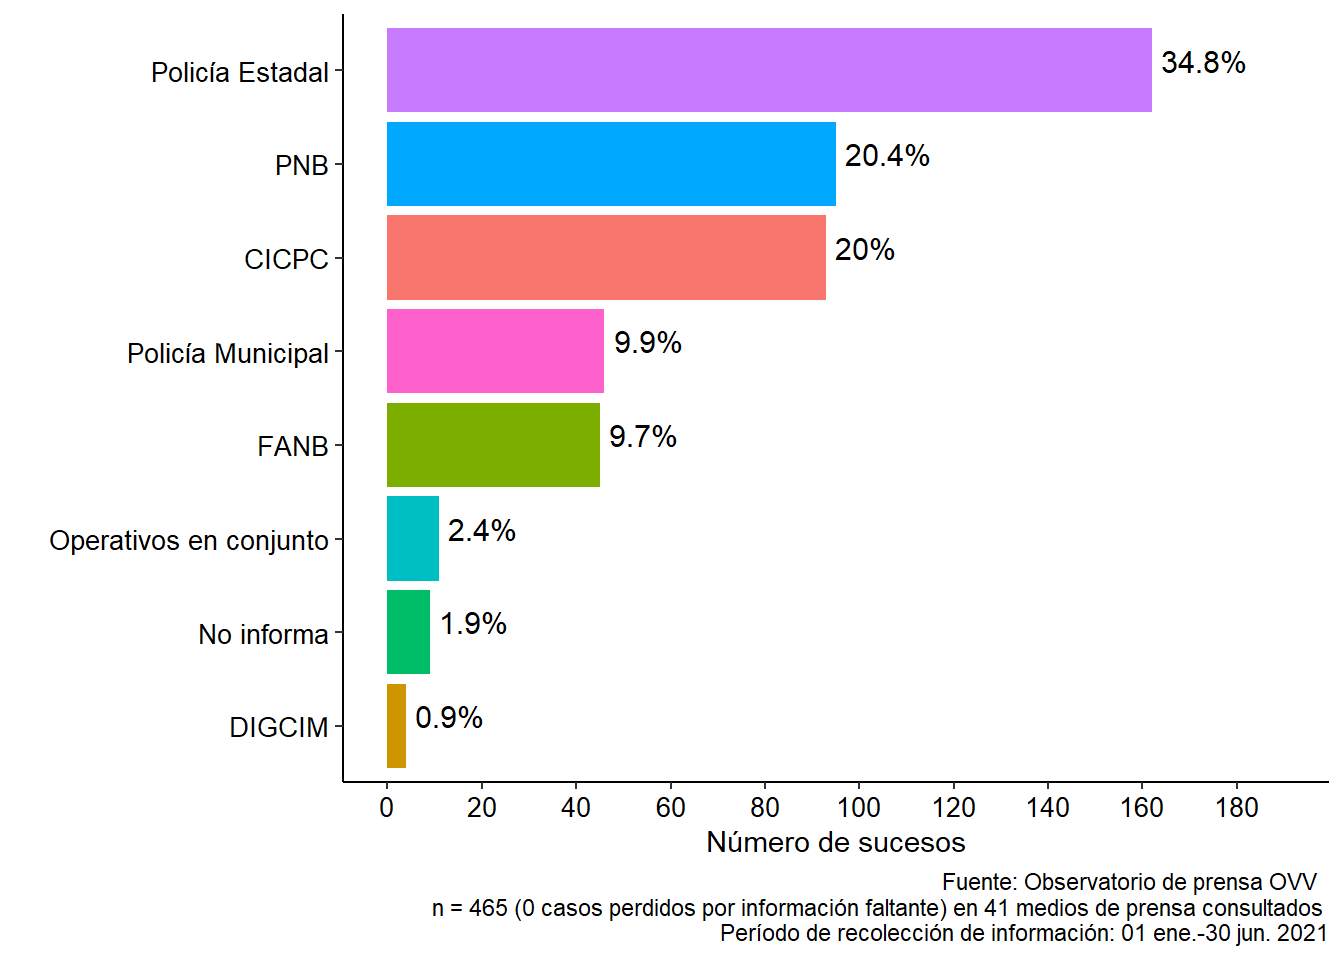
\includegraphics{bookdown-demo_files/figure-latex/sucesospol-1.pdf}
\caption{\label{fig:sucesospol}Número de sucesos por cuerpo de seguridad.}
\end{figure}

\hypertarget{sitio-de-ocurrencia}{%
\section{Sitio de ocurrencia}\label{sitio-de-ocurrencia}}



\begin{figure}
\centering
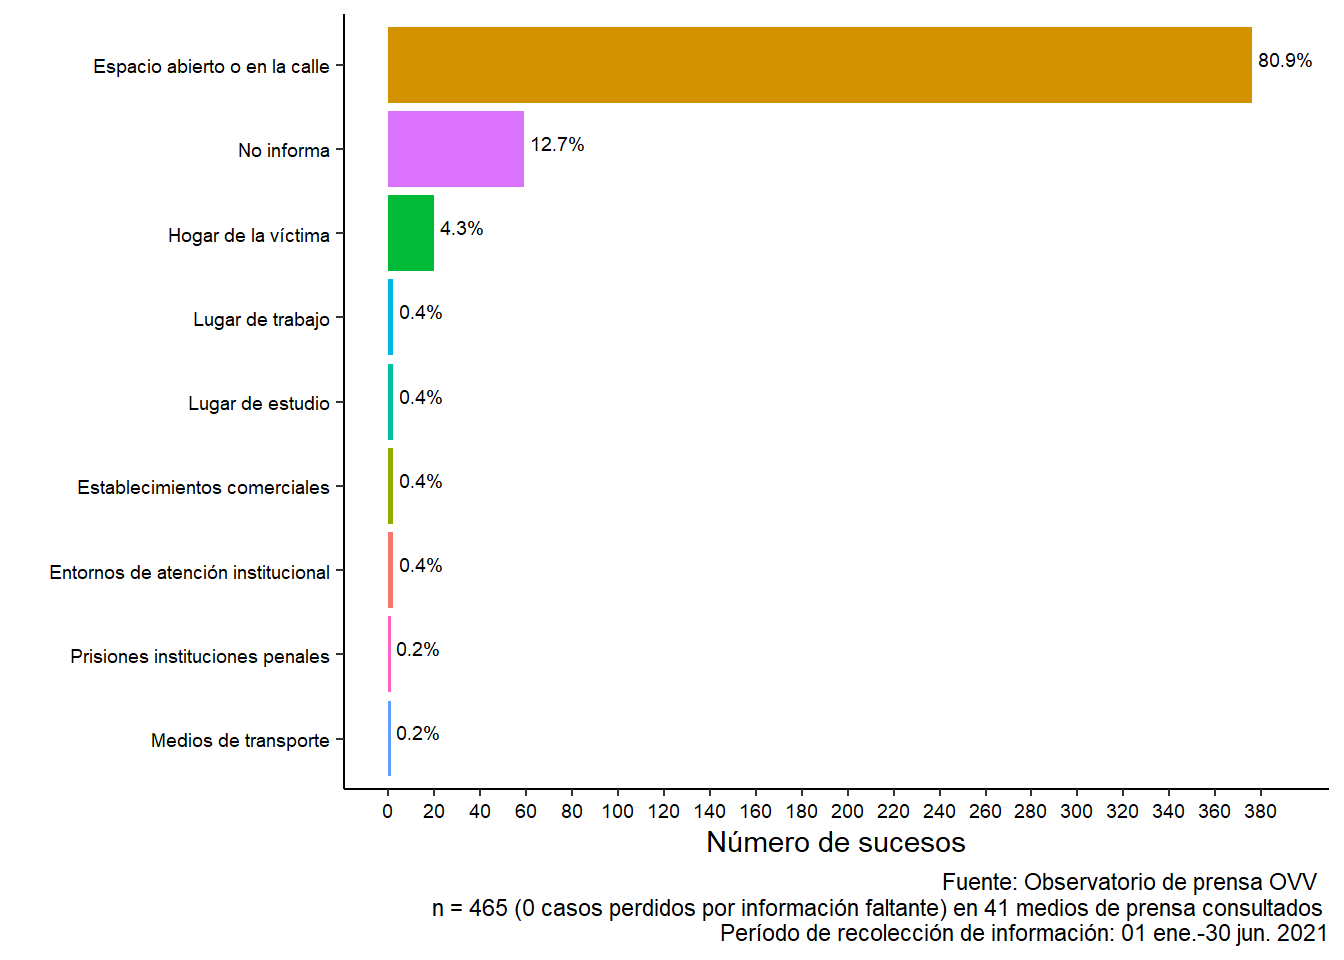
\includegraphics{bookdown-demo_files/figure-latex/sucesosmildondeplot-1.pdf}
\caption{\label{fig:sucesosmildondeplot}Número de sucesos y proporción de acuerdo al lugar donde ocurrió el evento.}
\end{figure}

\hypertarget{duxeda-de-ocurrencia}{%
\section{Día de ocurrencia}\label{duxeda-de-ocurrencia}}



\begin{figure}
\centering
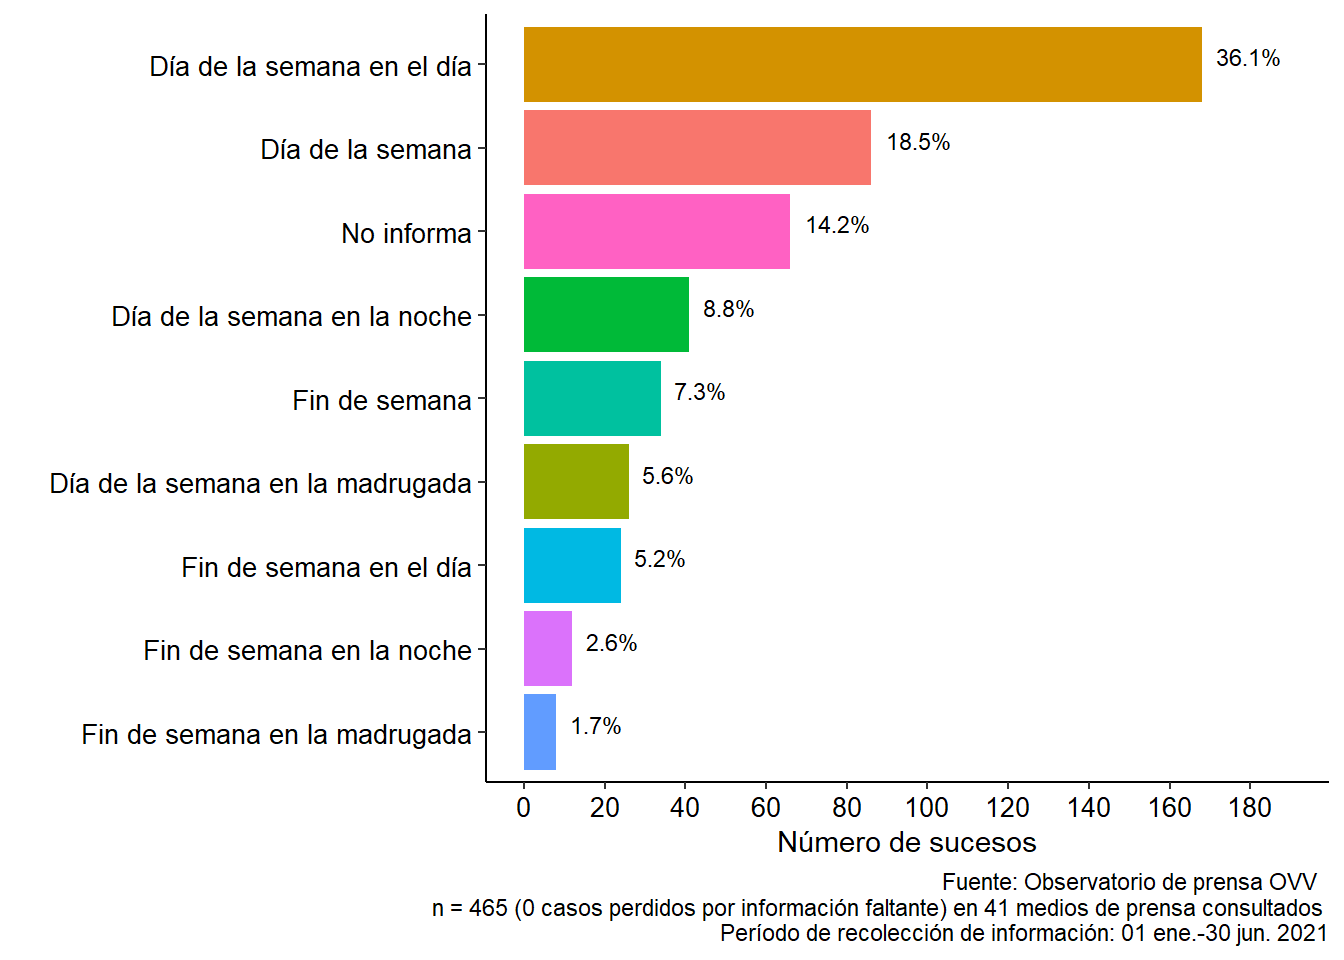
\includegraphics{bookdown-demo_files/figure-latex/sucesosmilcuandoplot-1.pdf}
\caption{\label{fig:sucesosmilcuandoplot}Número de sucesos y proporción de acuerdo al día en que ocurrió el evento.}
\end{figure}

\hypertarget{eventos-homicidio-intencional-hi}{%
\chapter{Eventos homicidio intencional (HI)}\label{eventos-homicidio-intencional-hi}}

\hypertarget{presunciuxf3n-del-codificador-hi}{%
\section{Presunción del codificador HI}\label{presunciuxf3n-del-codificador-hi}}

Nótese la alta cardinalidad de casos perdidos debido a información faltante, esto probablemente obedezca a que en la pregunta 31 del cuestionario una vez seleccionada la opción homicidio intencional, el sistema te indica pasar a la pregunta 34. Por esta razón, es posible que la mayoría de los codificadores dejen la casilla ``presunción del codificador'' (pregunta 32) vacía y, en consecuencia, el sistema la sustituye con un `NA'



\begin{figure}
\centering
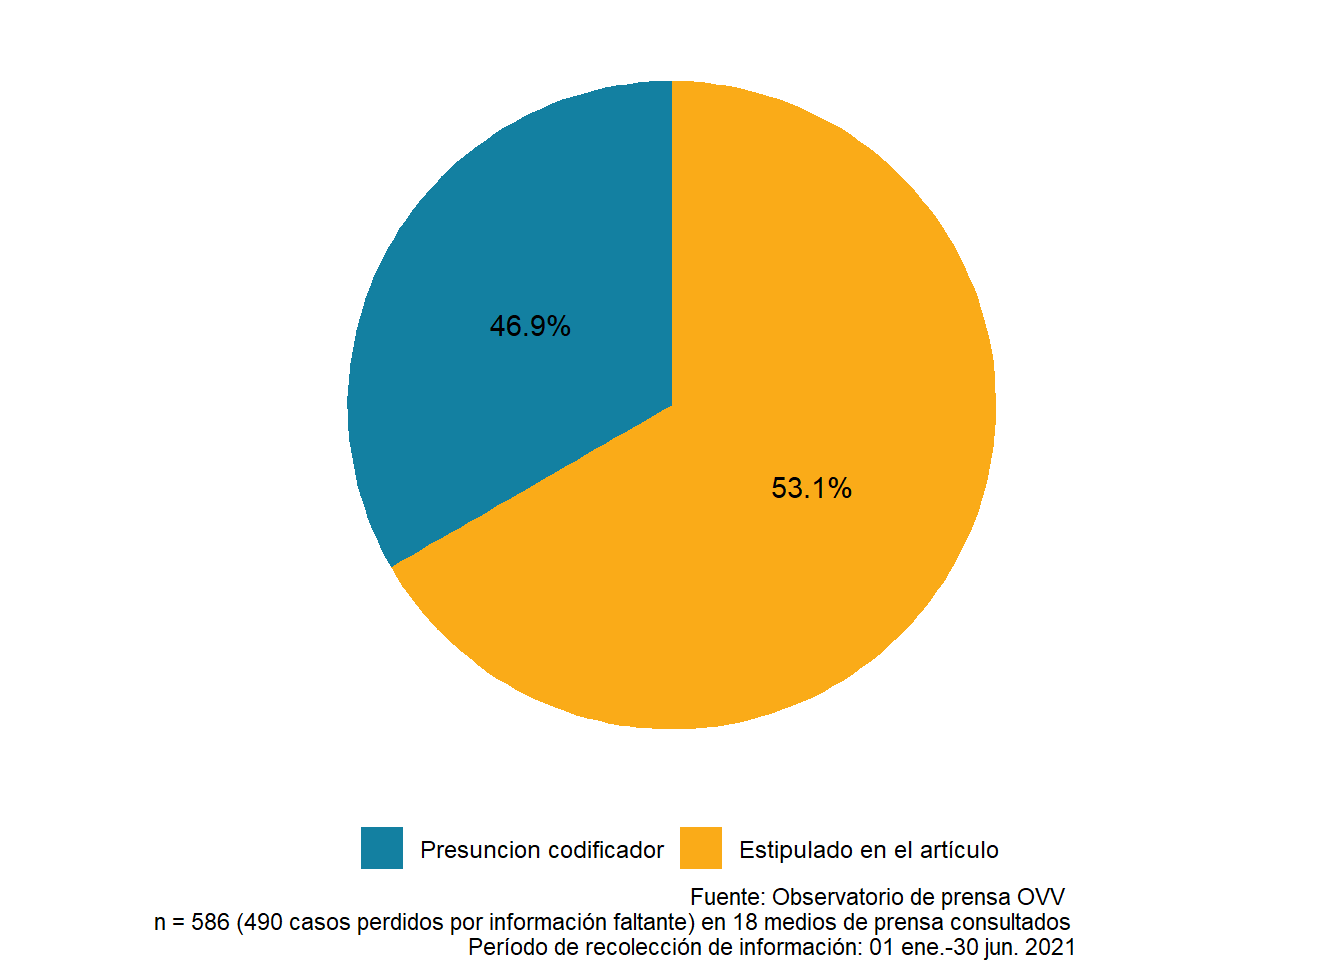
\includegraphics{bookdown-demo_files/figure-latex/sucesoshiprespiegraf-1.pdf}
\caption{\label{fig:sucesoshiprespiegraf}Número de sucesos discriminados según si la calificación como homicidio intencional es una presunción del codificador o si el artículo de prensa lo especifica claramente.}
\end{figure}

\hypertarget{tipo-de-muerte-hi}{%
\section{Tipo de muerte HI}\label{tipo-de-muerte-hi}}





\begin{figure}
\centering
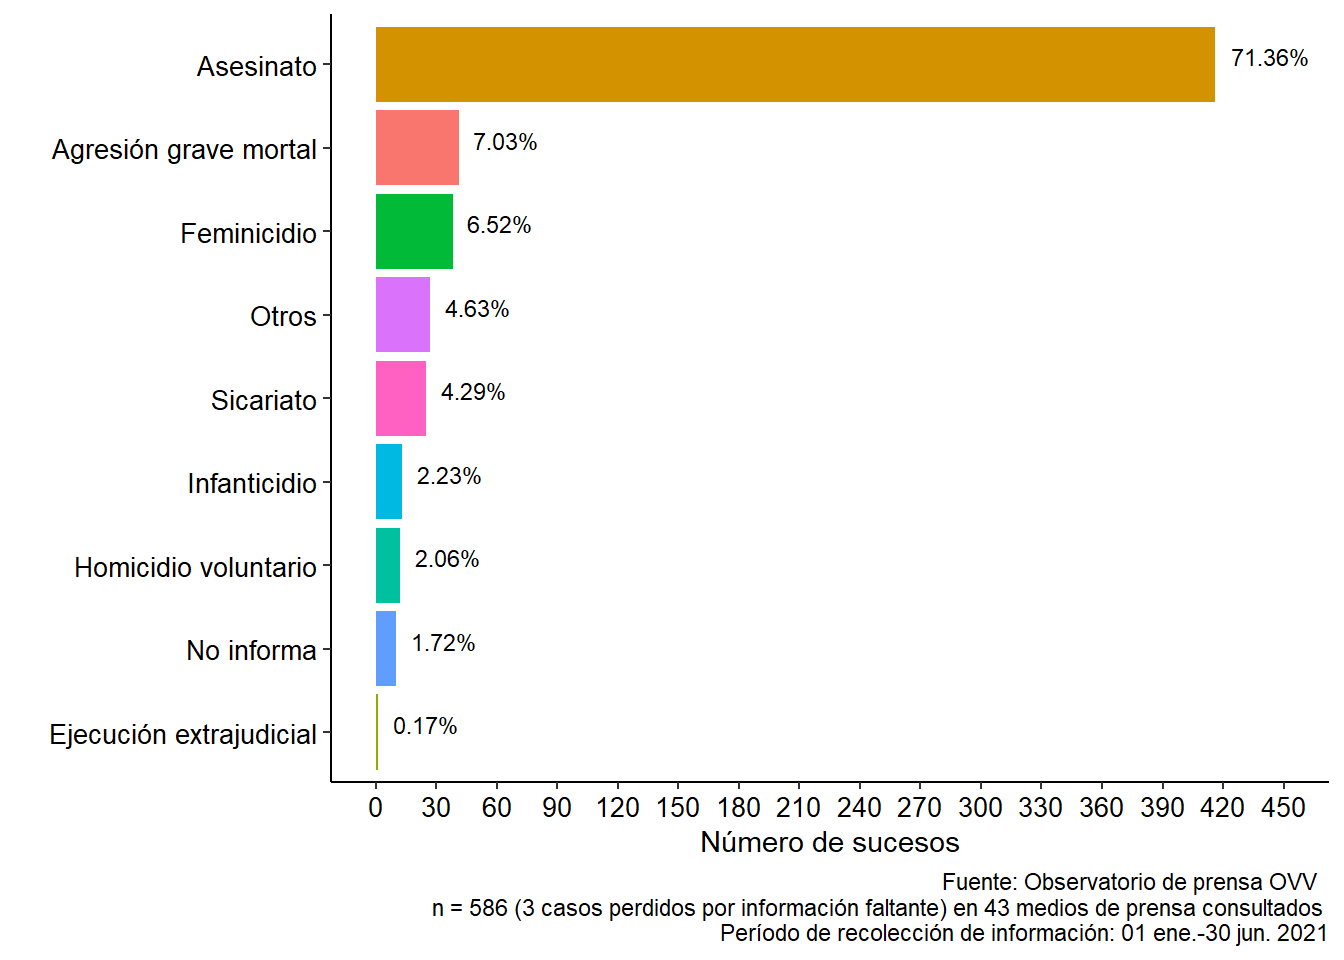
\includegraphics{bookdown-demo_files/figure-latex/sucesoshitipomubarragraf-1.pdf}
\caption{\label{fig:sucesoshitipomubarragraf}Número de sucesos para homicidio intencional discriminados según el tipo de muerte.}
\end{figure}

\begin{table}

\caption{\label{tab:sucesohitipomuhitable}Número de sucesos calificados como homicidio intencional discriminados por el tipo de muerte de las víctimas.}
\centering
\begin{tabular}[t]{lcr}
\toprule
Tipo de muerte & No. Sucesos & porcentaje\\
\midrule
Ejecución extrajudicial & 1 & 0.17\%\\
No informa & 10 & 1.72\%\\
Homicidio voluntario & 12 & 2.06\%\\
Infanticidio & 13 & 2.23\%\\
Sicariato & 25 & 4.29\%\\
\addlinespace
Otros & 27 & 4.63\%\\
Feminicidio & 38 & 6.52\%\\
Agresión grave mortal & 41 & 7.03\%\\
Asesinato & 416 & 71.36\%\\
\bottomrule
\end{tabular}
\end{table}

\begin{figure}
\centering
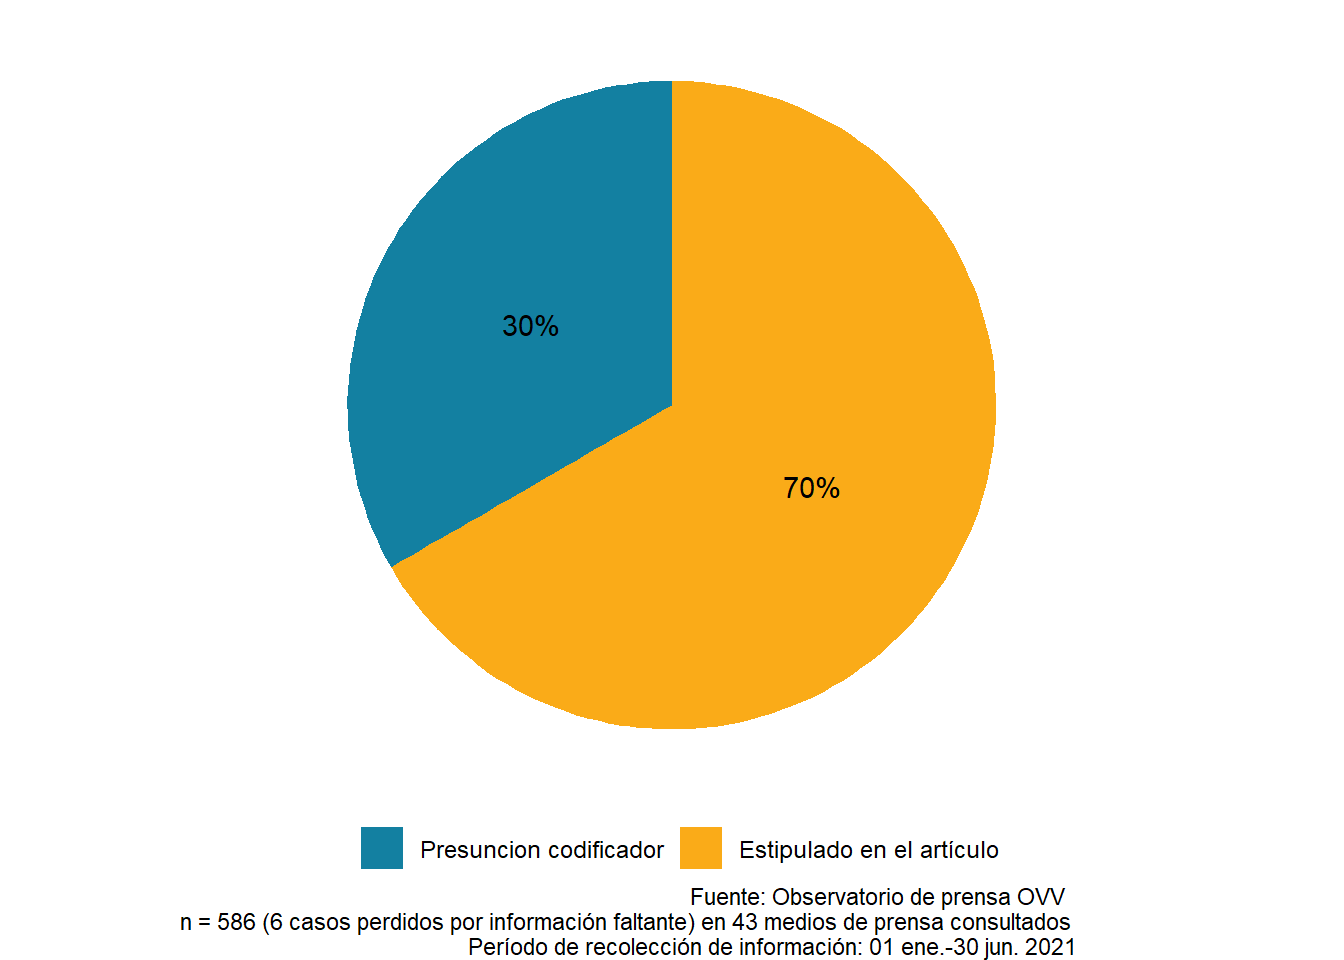
\includegraphics{bookdown-demo_files/figure-latex/sucesoshitipomupres35piegraf-1.pdf}
\caption{\label{fig:sucesoshitipomupres35piegraf}Número de sucesos discriminados según si la calificación del tipo de muerte corresponde a una presunción del codificador o si el artículo de prensa lo especifica claramente.}
\end{figure}

\hypertarget{nuxfamero-de-vuxedctimas-hi}{%
\section{Número de víctimas HI}\label{nuxfamero-de-vuxedctimas-hi}}



\begin{figure}
\centering
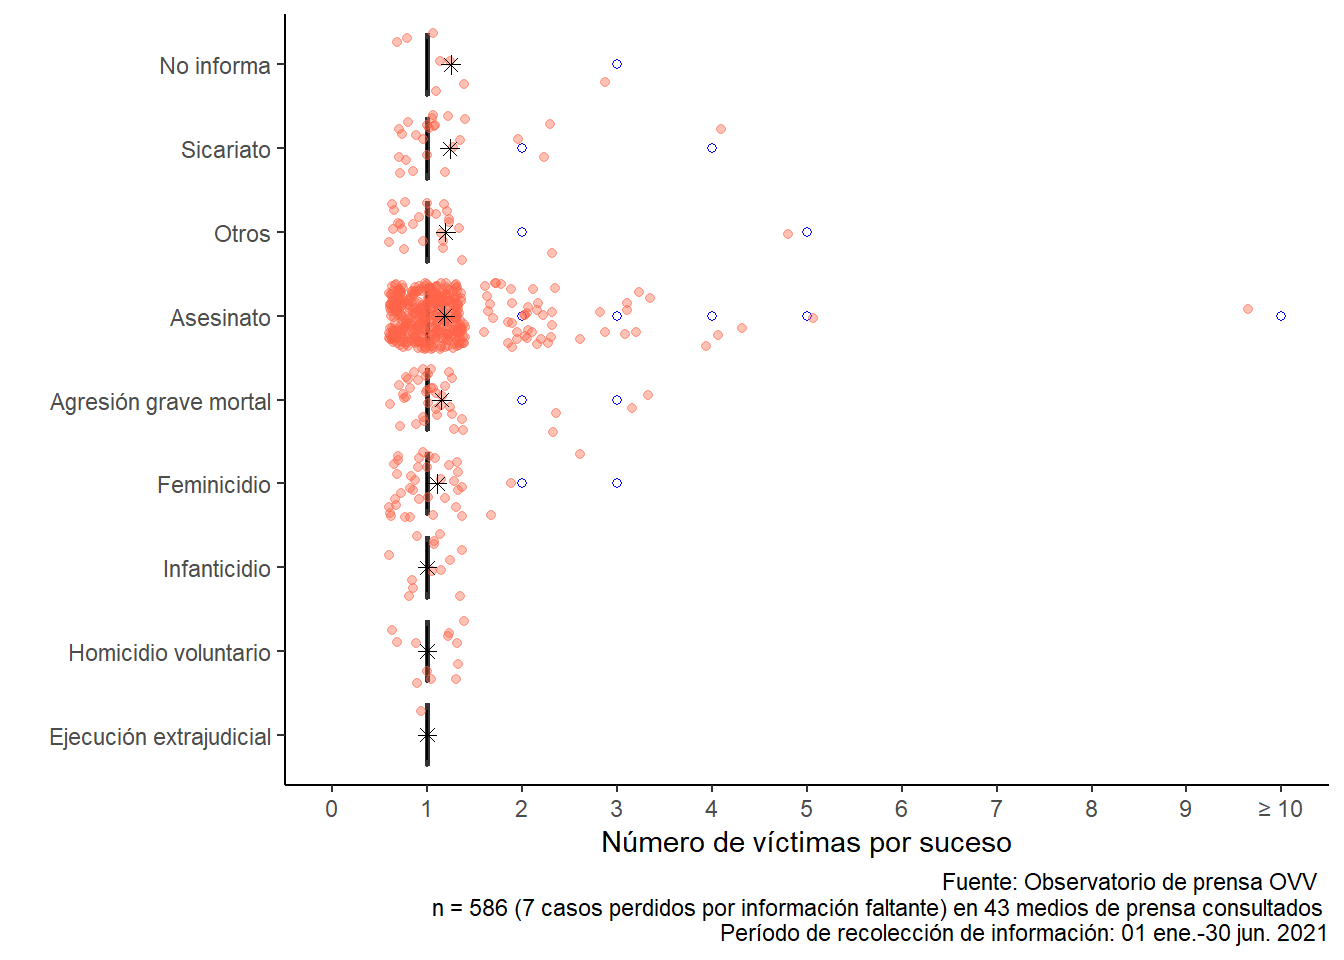
\includegraphics{bookdown-demo_files/figure-latex/sucesoshitipomuboxplotgraf-1.pdf}
\caption{\label{fig:sucesoshitipomuboxplotgraf}Número de víctimas por suceso para homicidio intencional discriminados según el tipo de muerte.}
\end{figure}

\hypertarget{nuxfamero-de-victimario-hi}{%
\section{Número de victimario HI}\label{nuxfamero-de-victimario-hi}}



\begin{figure}
\centering
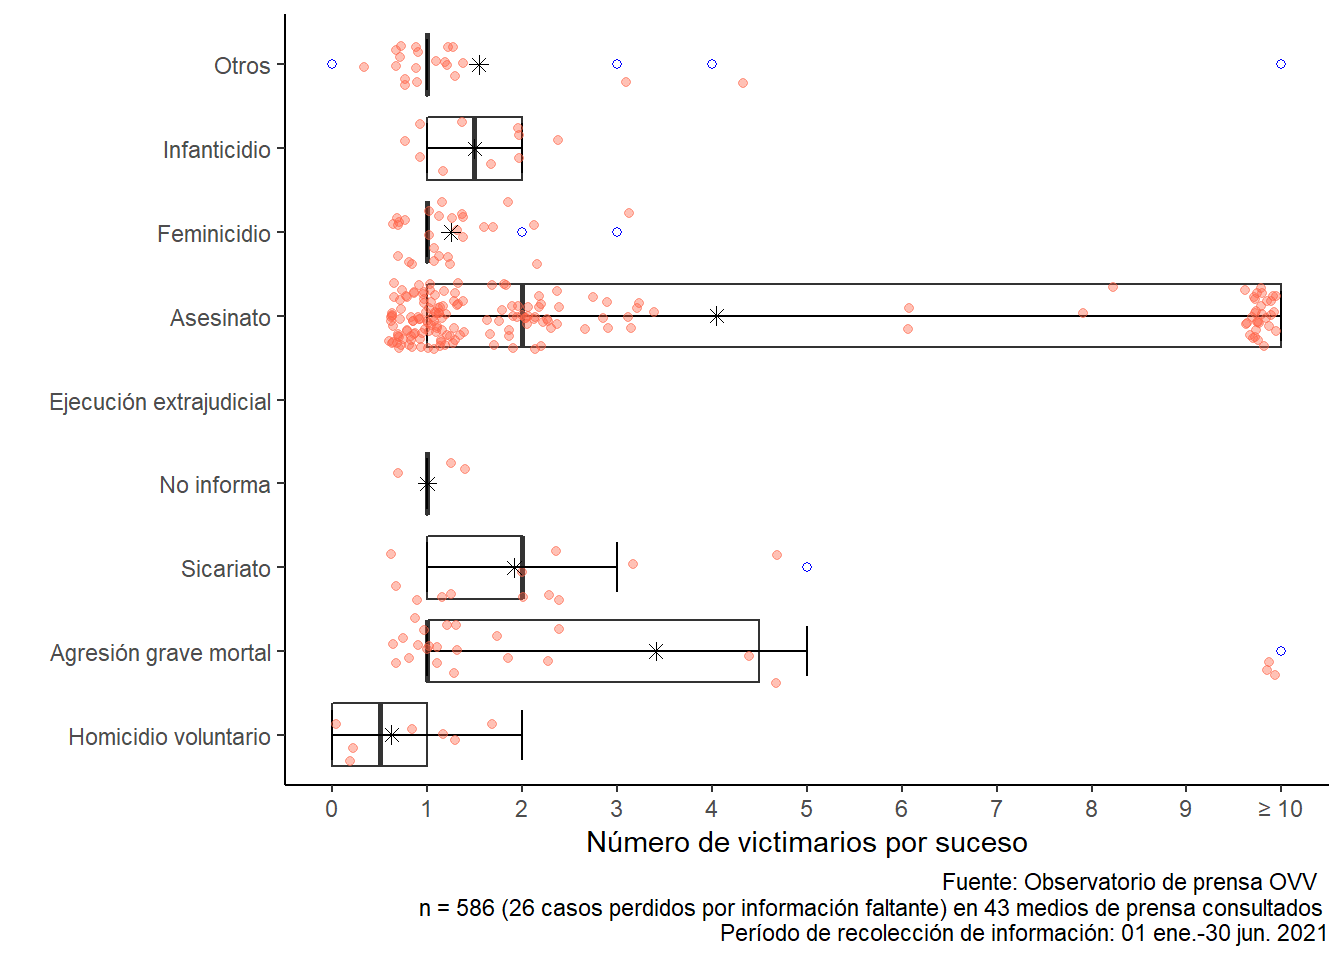
\includegraphics{bookdown-demo_files/figure-latex/sucesoshitipomuvictimarioboxplotgraf-1.pdf}
\caption{\label{fig:sucesoshitipomuvictimarioboxplotgraf}Número de victimarios por suceso de homicidio intencional discriminados según el tipo de muerte. Media: *; mediana: \textbar; valor atípico: ○.}
\end{figure}

\hypertarget{duxeda-de-ocurrencia-hi}{%
\section{Día de ocurrencia HI}\label{duxeda-de-ocurrencia-hi}}



\begin{figure}
\centering
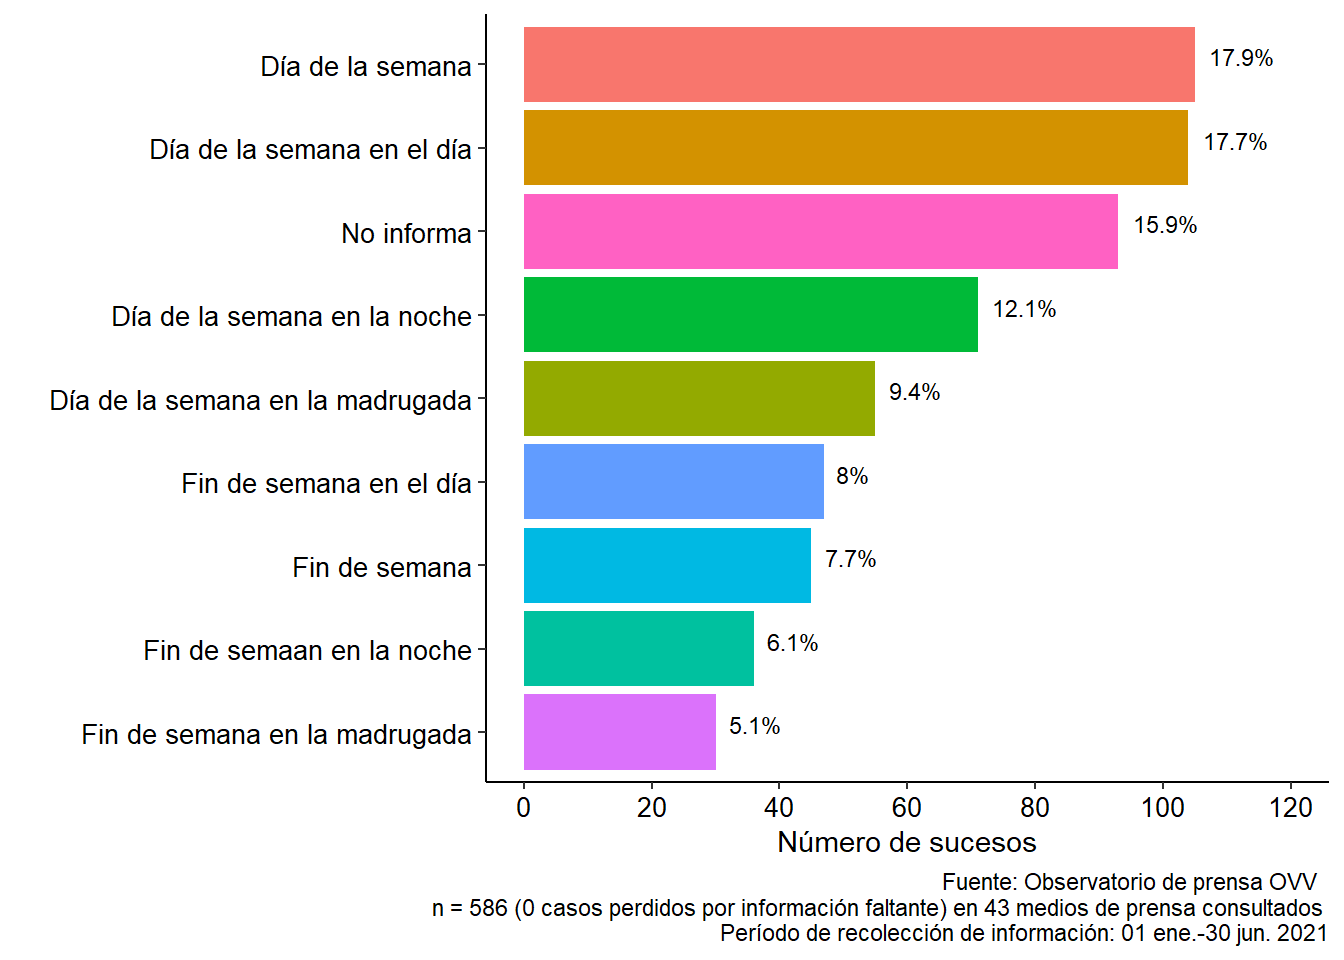
\includegraphics{bookdown-demo_files/figure-latex/sucesoshicuandobarrasgraf-1.pdf}
\caption{\label{fig:sucesoshicuandobarrasgraf}Número de sucesos de de homicidio intencional discriminados según día de ocurrencia.}
\end{figure}

\hypertarget{sitio-de-ocurrencia-del-hi}{%
\section{Sitio de ocurrencia del HI}\label{sitio-de-ocurrencia-del-hi}}



\begin{figure}
\centering
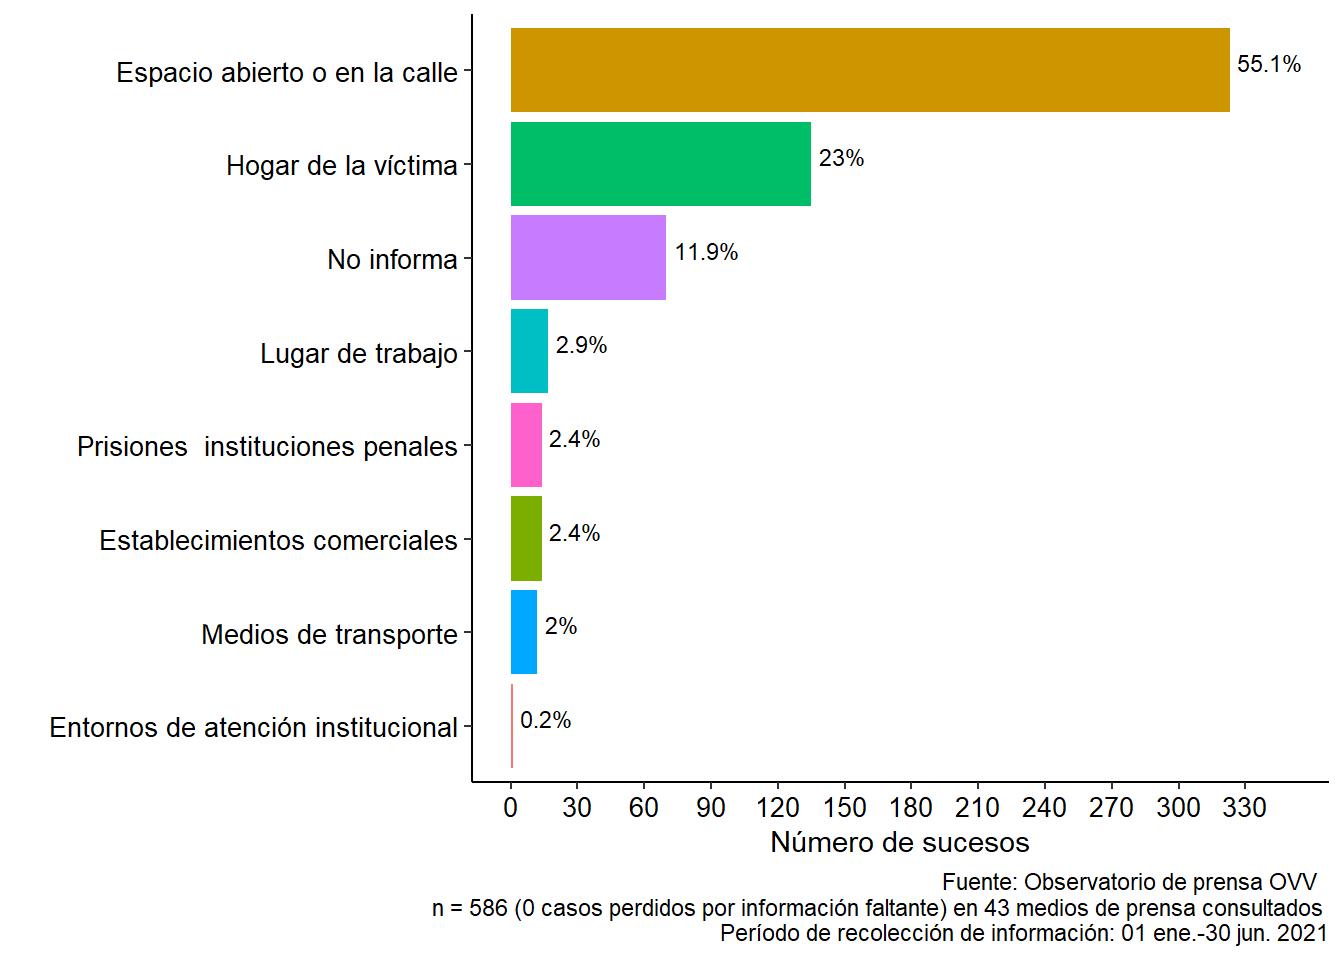
\includegraphics{bookdown-demo_files/figure-latex/sucesoshidondebarrasgraf-1.pdf}
\caption{\label{fig:sucesoshidondebarrasgraf}Número de sucesos de homicidio intencional discriminados según el sitio de ocurrencia.}
\end{figure}



\begin{figure}
\centering
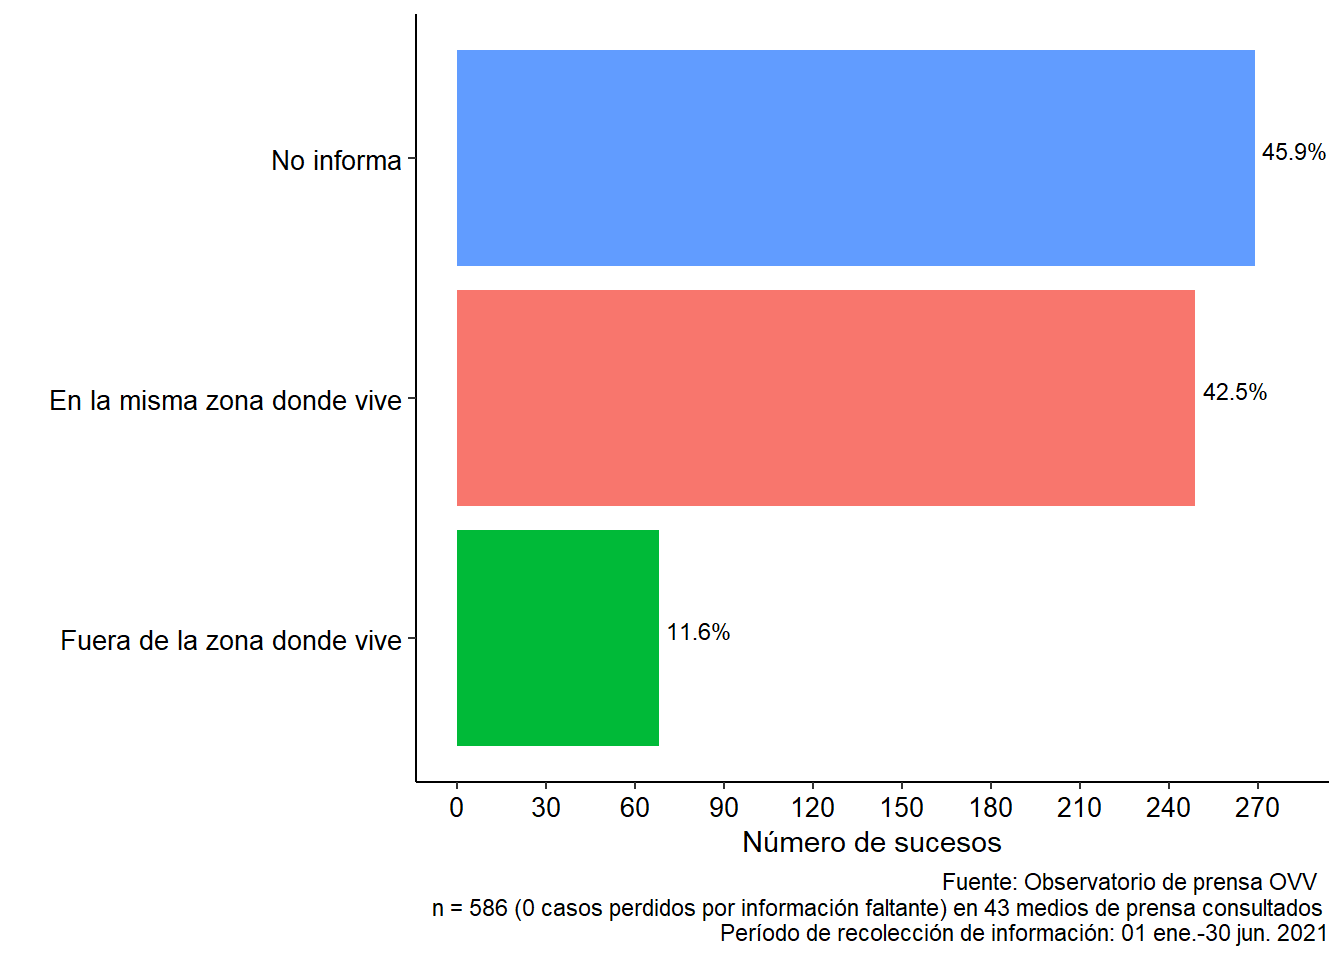
\includegraphics{bookdown-demo_files/figure-latex/sucesoshicercaniabarrasgraf-1.pdf}
\caption{\label{fig:sucesoshicercaniabarrasgraf}Número de sucesos de homicidio intencional discriminados según cercanía al sitio donde vivia la víctima.}
\end{figure}

\hypertarget{tipo-de-arma}{%
\section{Tipo de arma}\label{tipo-de-arma}}



\begin{figure}
\centering
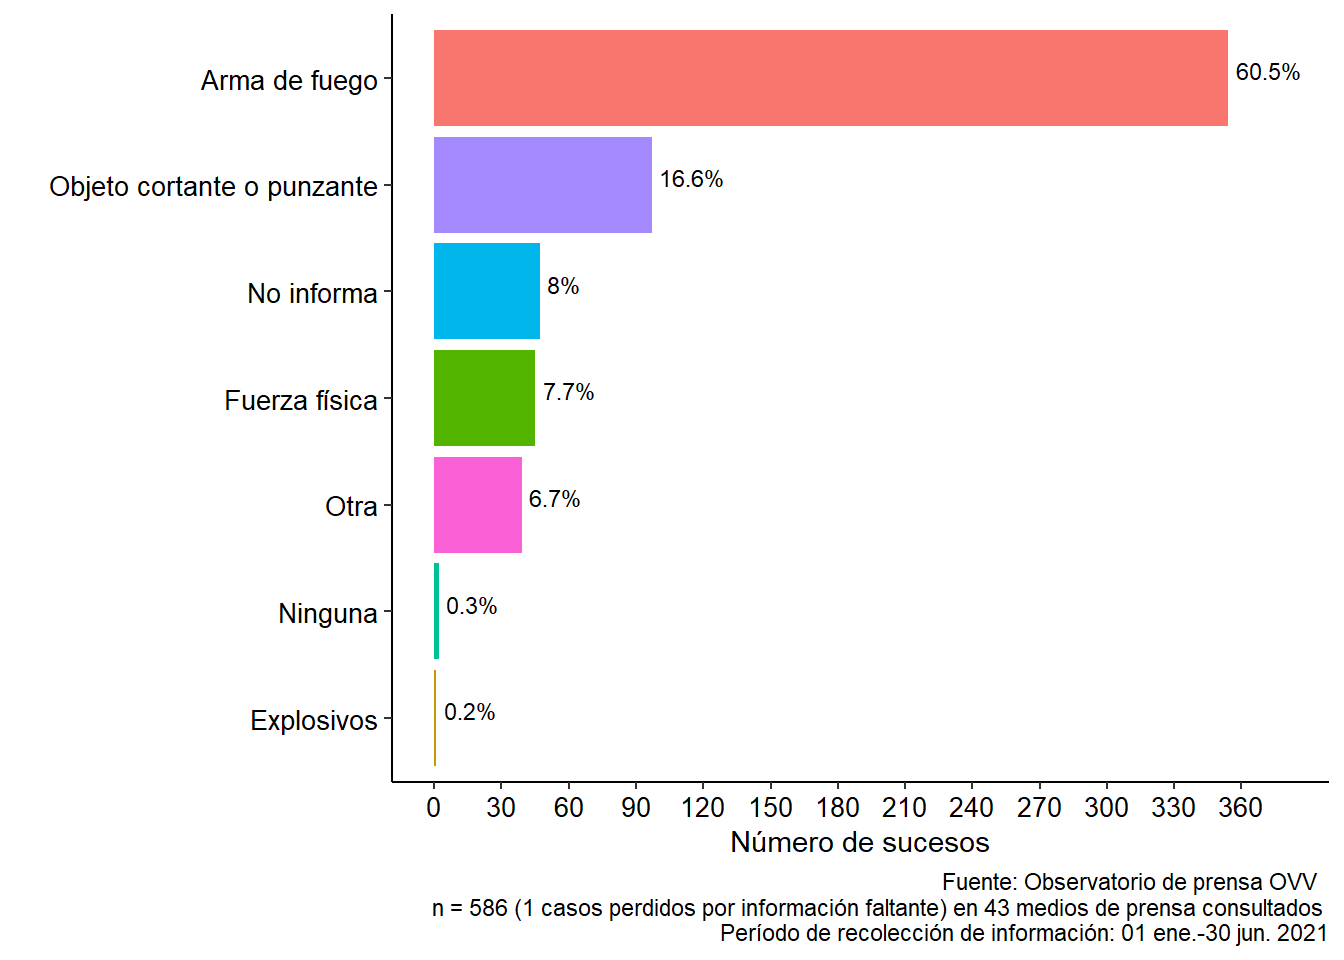
\includegraphics{bookdown-demo_files/figure-latex/sucesoshitipoarmabarrasgraf-1.pdf}
\caption{\label{fig:sucesoshitipoarmabarrasgraf}Número de sucesos de homicidio intencional discriminados según el tipo de arma utilizada.}
\end{figure}

\hypertarget{quiuxe9n-fue-el-victimario}{%
\section{¿Quién fue el victimario?}\label{quiuxe9n-fue-el-victimario}}



\begin{figure}
\centering
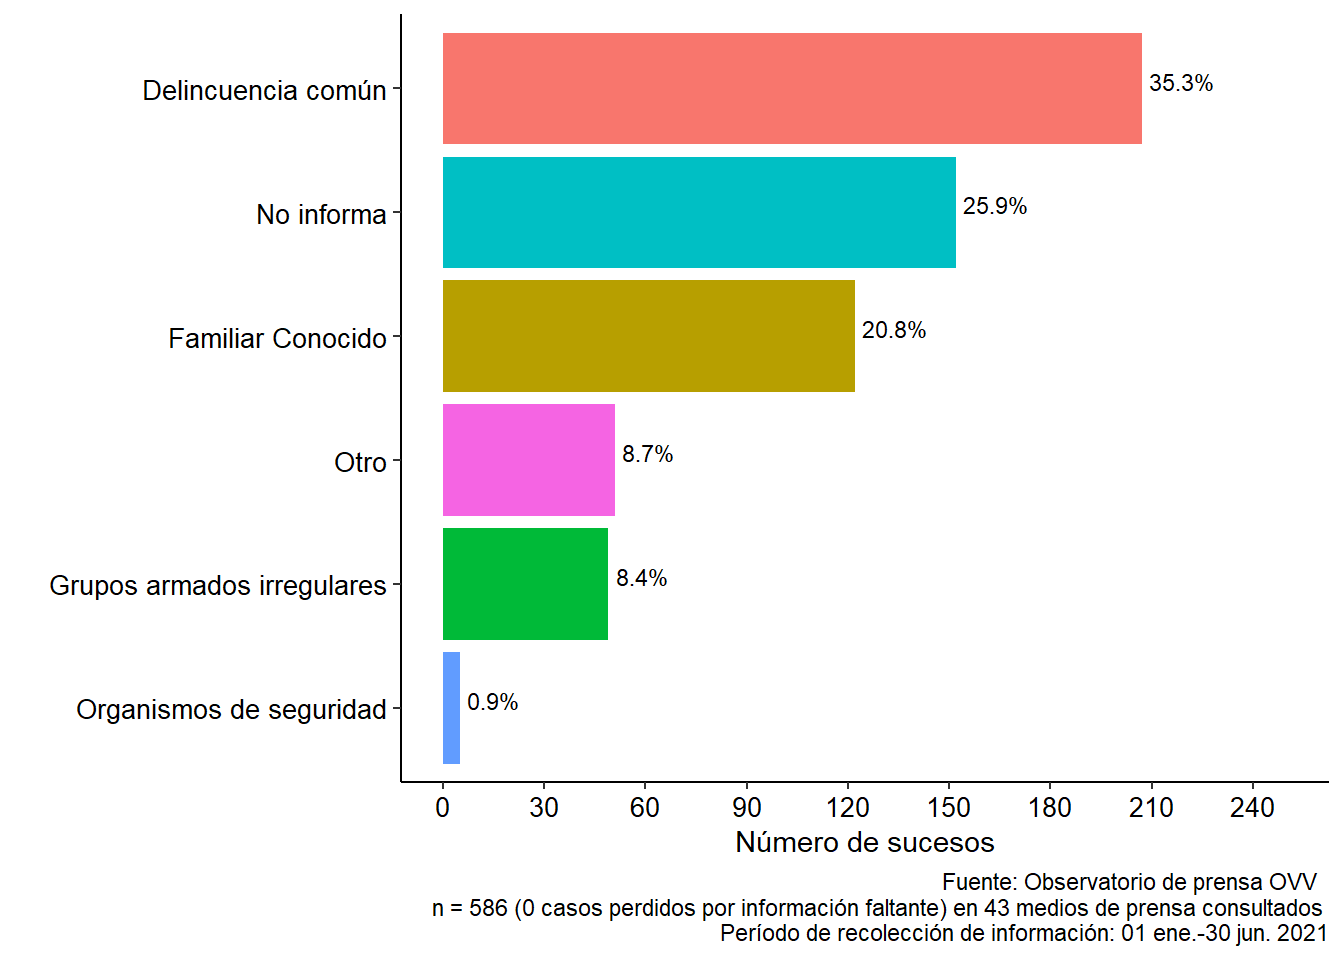
\includegraphics{bookdown-demo_files/figure-latex/sucesoshiquienvictimariobarrasgraf-1.pdf}
\caption{\label{fig:sucesoshiquienvictimariobarrasgraf}Número de sucesos de homicidio intencional discriminados según quién fue el victimario.}
\end{figure}

\hypertarget{conocido-o-familiar}{%
\subsection{¿Conocido o familiar?}\label{conocido-o-familiar}}

En este caso la alta cardinalidad de casos perdidos (456) no debe sorprender ya que la opción ``familiar/conocido'' de la pregunta No.~58 constituye un subconjunto (130) de los casos de homicidio intencional como se puede ver en la Figura \ref{fig:sucesoshiquienvictimariobarrasgraf}. En consecuencia, cuando el codificador selecciona esta opción, el sistema le atribuye un ``NA'' a todos aquellos sucesos que no encajen dentro de esta categoría.



\begin{figure}
\centering
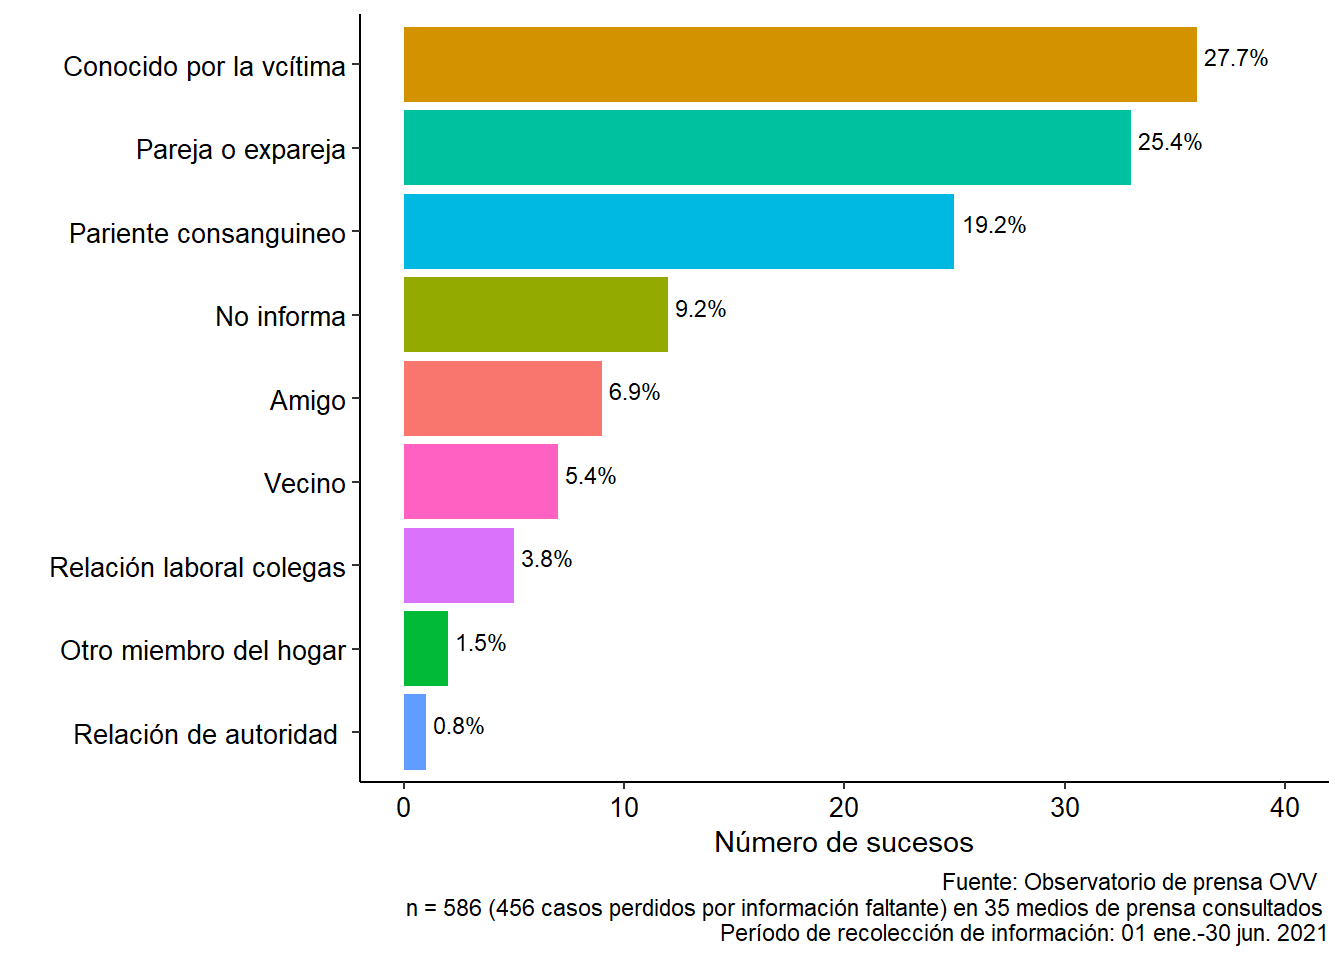
\includegraphics{bookdown-demo_files/figure-latex/sucesoshiconocidofamiliearvictimariobarrasgraf-1.pdf}
\caption{\label{fig:sucesoshiconocidofamiliearvictimariobarrasgraf}Número de sucesos de homicidio intencional discriminados según si el victimario era conocido o familiar\footnote{En este caso la alta cardinalidad de casos perdidos (456) no debe sorprender ya que la opción ``familiar/conocido'' de la pregunta No.~58 constituye un subconjunto (130) de los casos de homicidio intencional como se puede ver en la Figura \ref{fig:sucesoshiquienvictimariobarrasgraf}. En consecuencia, cuando el codificador selecciona esta opción, el sistema le atribuye un ``NA'' a todos aquellos sucesos que no encajen dentro de esta categoría.}.}
\end{figure}

\hypertarget{victimario-funcionario-de-seguridad}{%
\section{Victimario funcionario de seguridad}\label{victimario-funcionario-de-seguridad}}



\begin{figure}
\centering
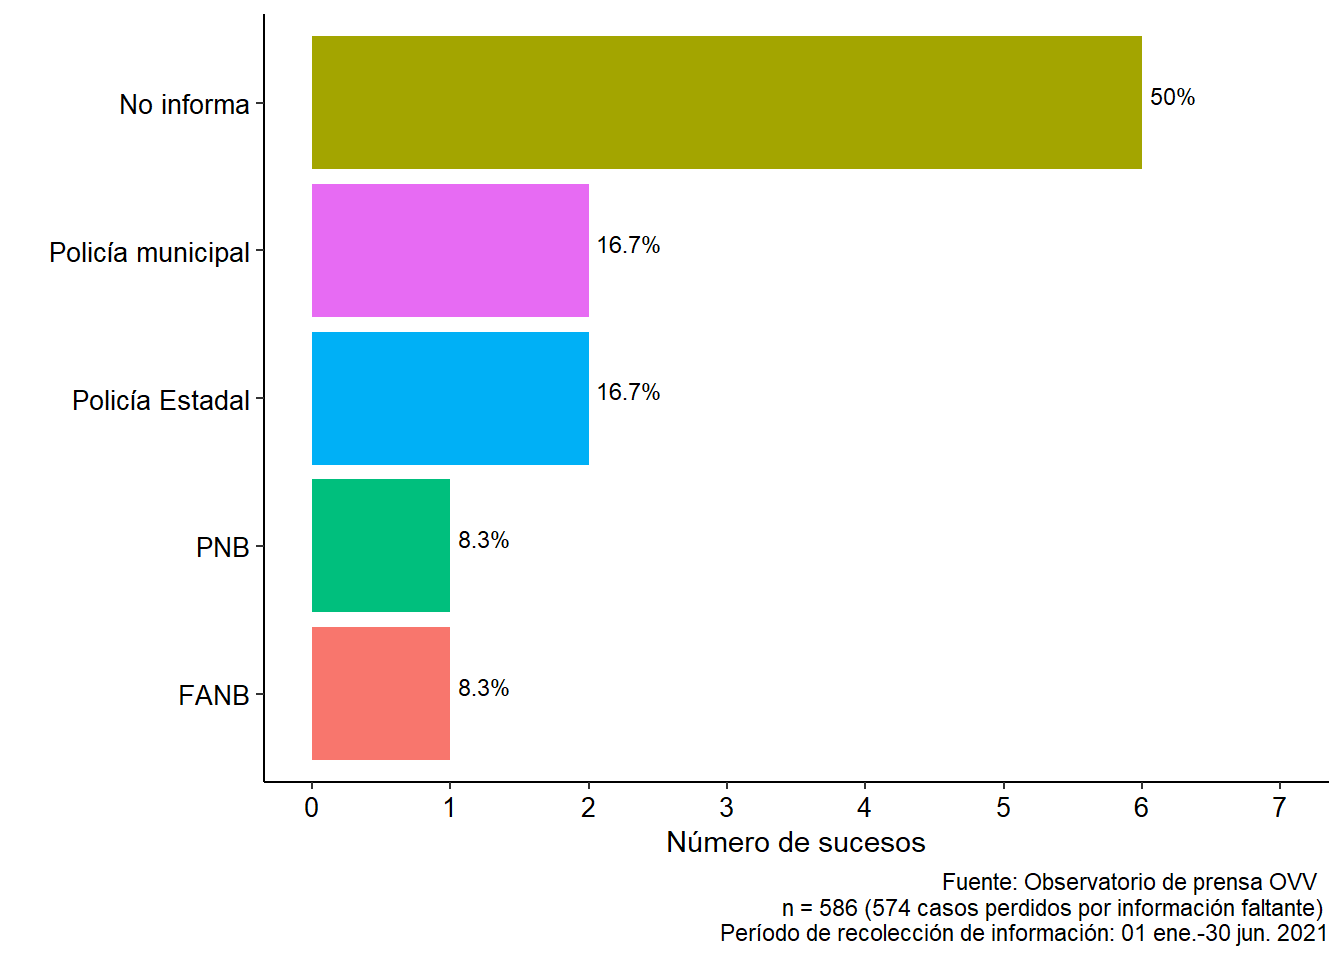
\includegraphics{bookdown-demo_files/figure-latex/sucesoshicuerposeguridadvictimariobarrasgraf-1.pdf}
\caption{\label{fig:sucesoshicuerposeguridadvictimariobarrasgraf}Número de sucesos de homicidio intencional discriminados según el cuerpo de seguridad al que pertenece el victimario.}
\end{figure}

\hypertarget{con-que-se-relaciona-el-homicidio}{%
\section{¿Con que se relaciona el homicidio?}\label{con-que-se-relaciona-el-homicidio}}



\begin{figure}
\centering
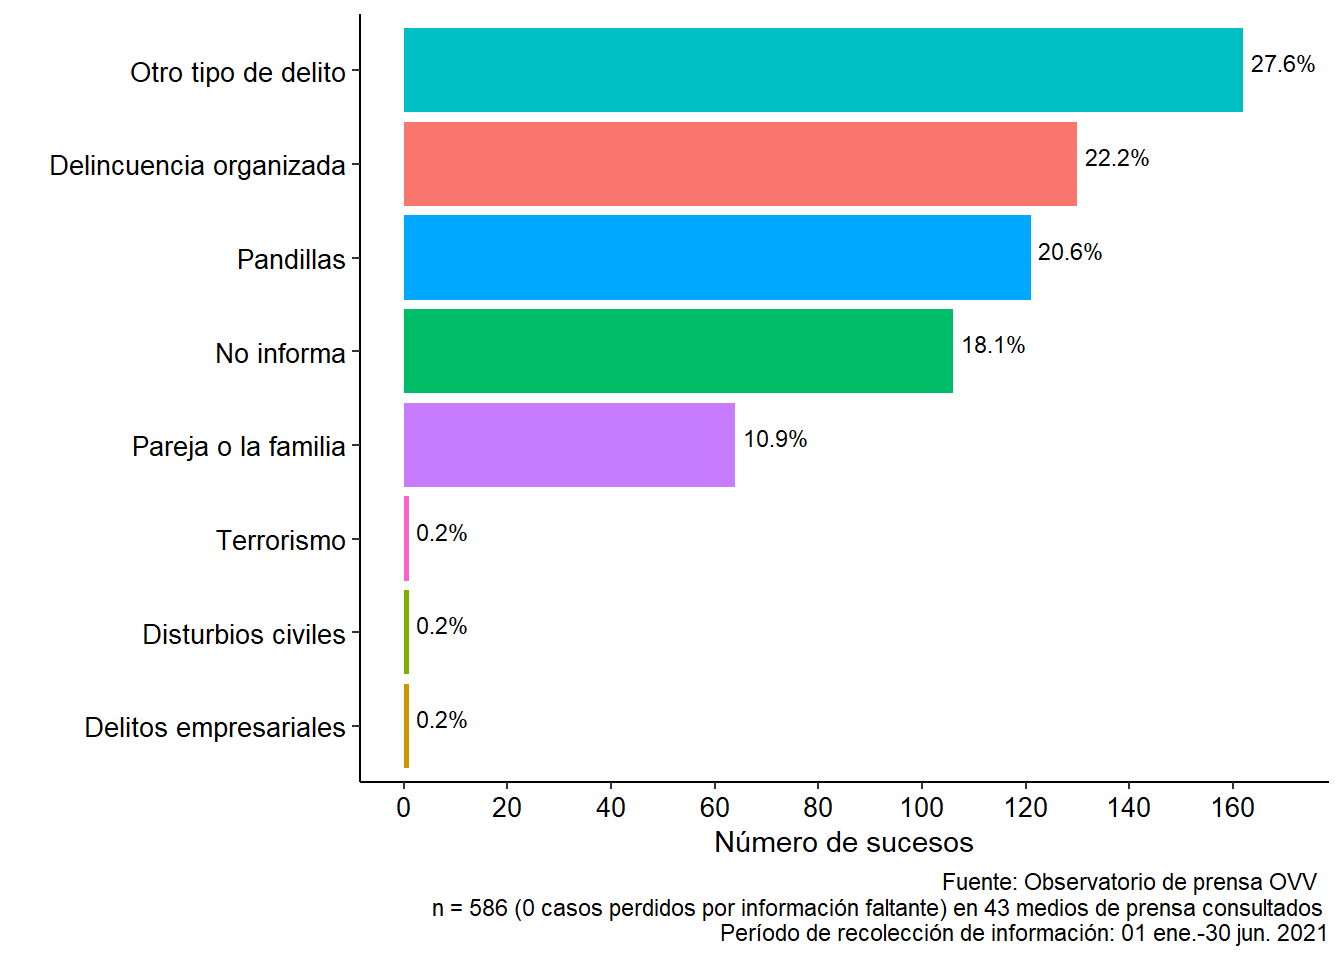
\includegraphics{bookdown-demo_files/figure-latex/sucesoshiconquerelacionahibarrasgraf-1.pdf}
\caption{\label{fig:sucesoshiconquerelacionahibarrasgraf}Número de sucesos de homicidio intencional discriminados según el contexto del suceso.}
\end{figure}

\hypertarget{contexto-del-homicidio-intencional}{%
\section{Contexto del homicidio intencional}\label{contexto-del-homicidio-intencional}}



\begin{figure}
\centering
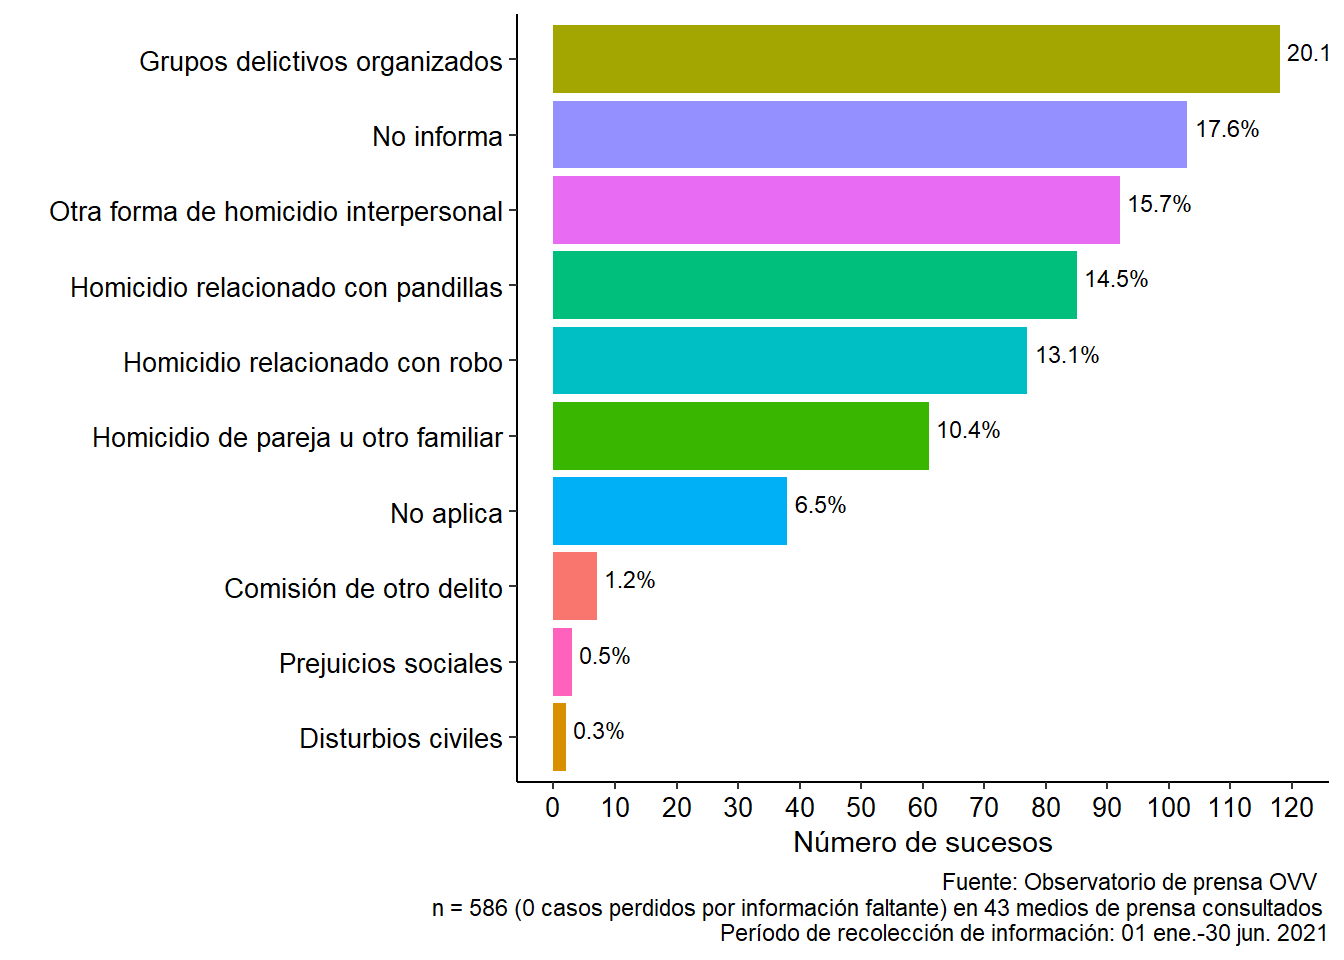
\includegraphics{bookdown-demo_files/figure-latex/sucesoshicontextohibarrasgraf-1.pdf}
\caption{\label{fig:sucesoshicontextohibarrasgraf}Número de sucesos de homicidio intencional discriminados según el contexto del homicidio.}
\end{figure}

\hypertarget{presuncion-del-contexto}{%
\section{Presuncion del contexto}\label{presuncion-del-contexto}}



\begin{figure}
\centering
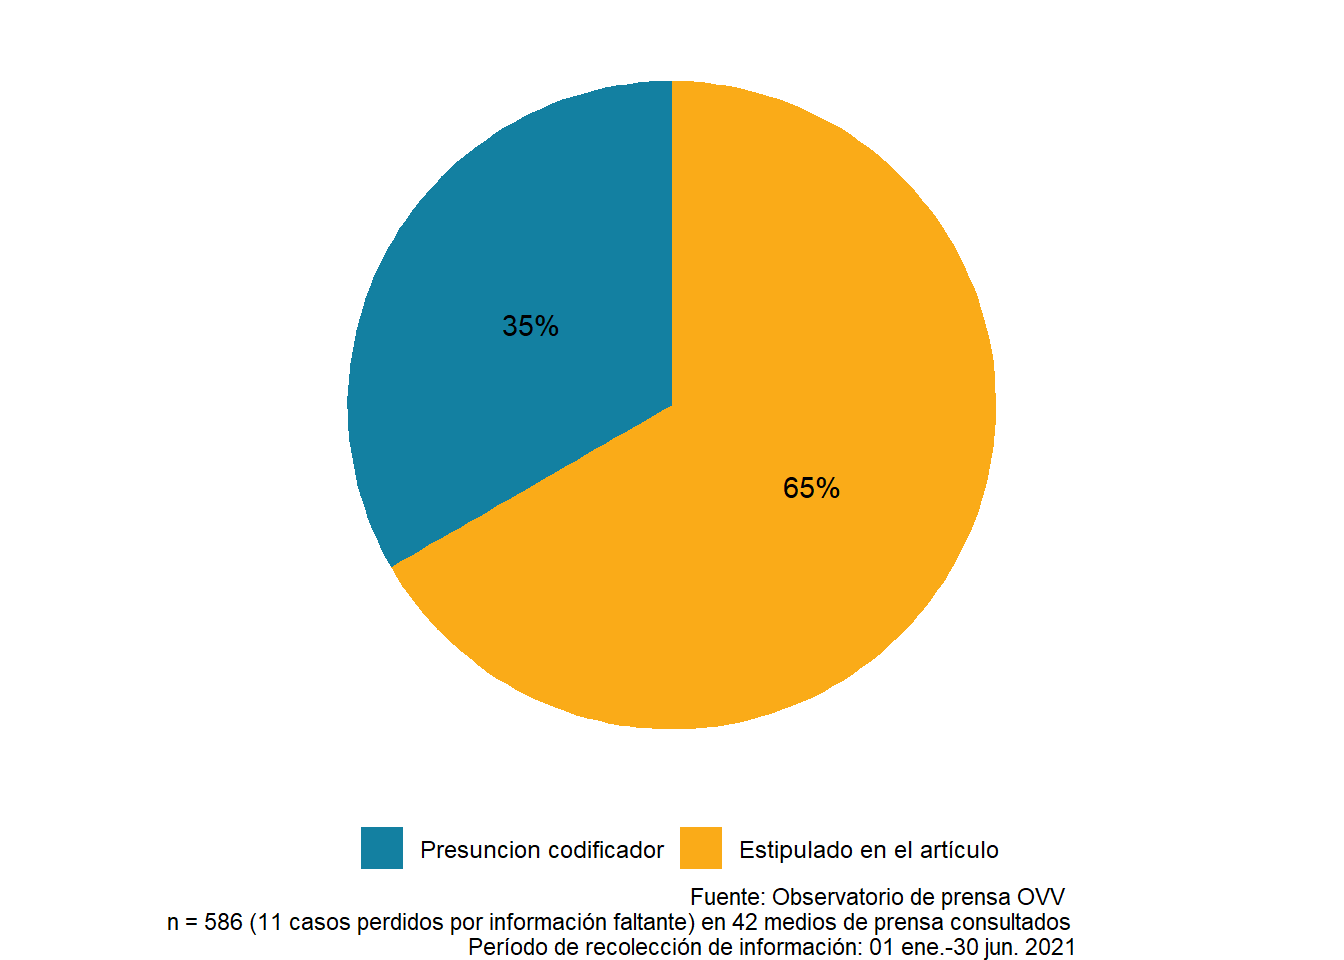
\includegraphics{bookdown-demo_files/figure-latex/sucesoshiprescontextohipiegraf-1.pdf}
\caption{\label{fig:sucesoshiprescontextohipiegraf}Proporción de sucesos de homicidio intencional discriminados si el contexto del homicidio es presunción del codificador o estipulado en el artículo de prensa.}
\end{figure}

\hypertarget{motivaciuxf3n-del-homicidio-intencional}{%
\section{Motivación del homicidio intencional}\label{motivaciuxf3n-del-homicidio-intencional}}



\begin{figure}
\centering
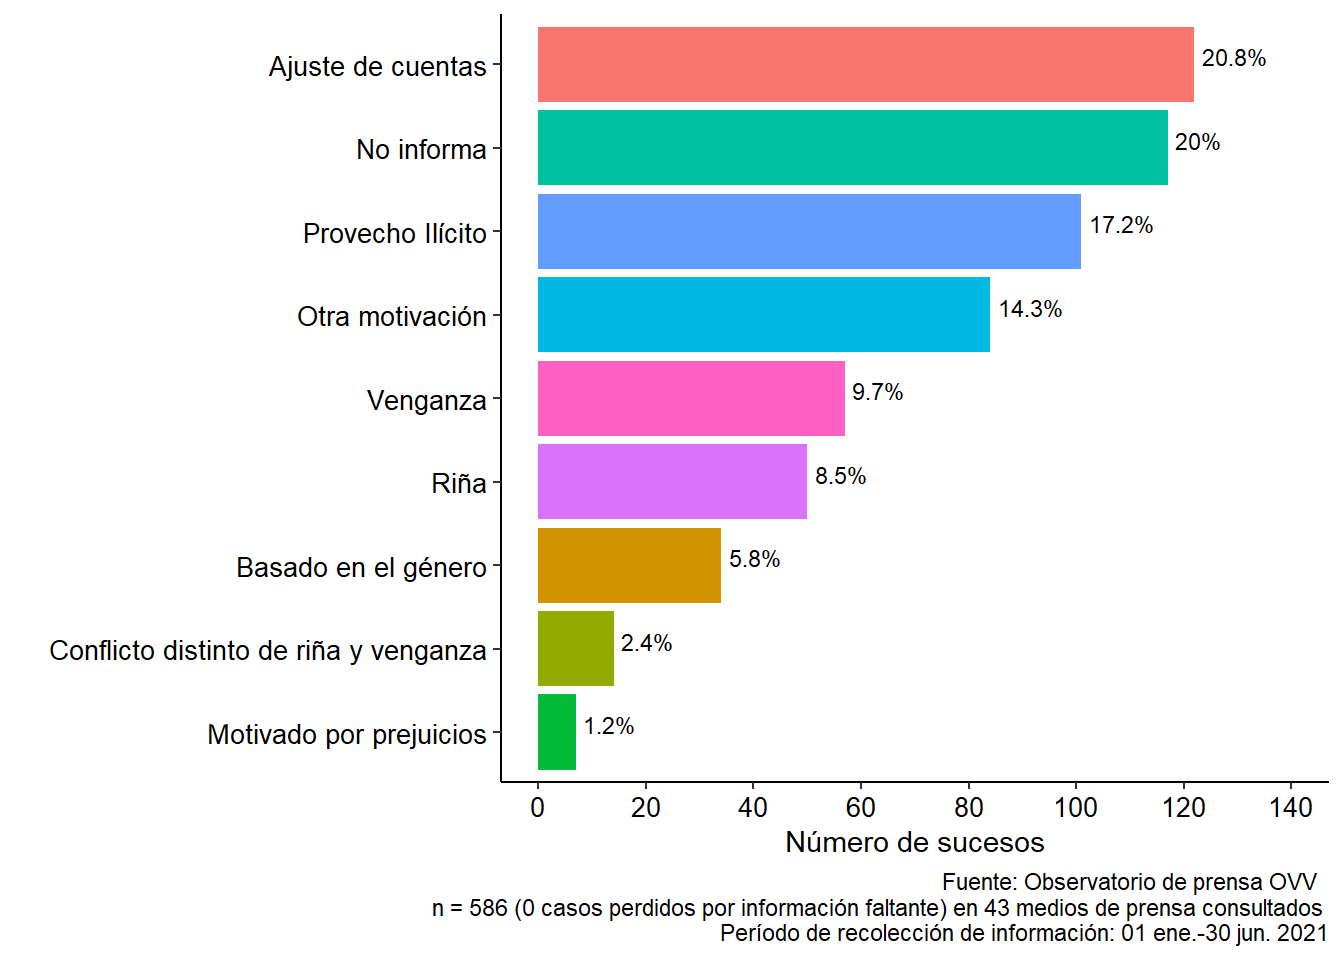
\includegraphics{bookdown-demo_files/figure-latex/sucesoshimotivacionhibarragraf-1.pdf}
\caption{\label{fig:sucesoshimotivacionhibarragraf}Número de sucesos de homicidio intencional discriminados según su motivación.}
\end{figure}

\hypertarget{presunciuxf3n-de-la-motivaciuxf3n}{%
\section{Presunción de la motivación}\label{presunciuxf3n-de-la-motivaciuxf3n}}



\begin{figure}
\centering
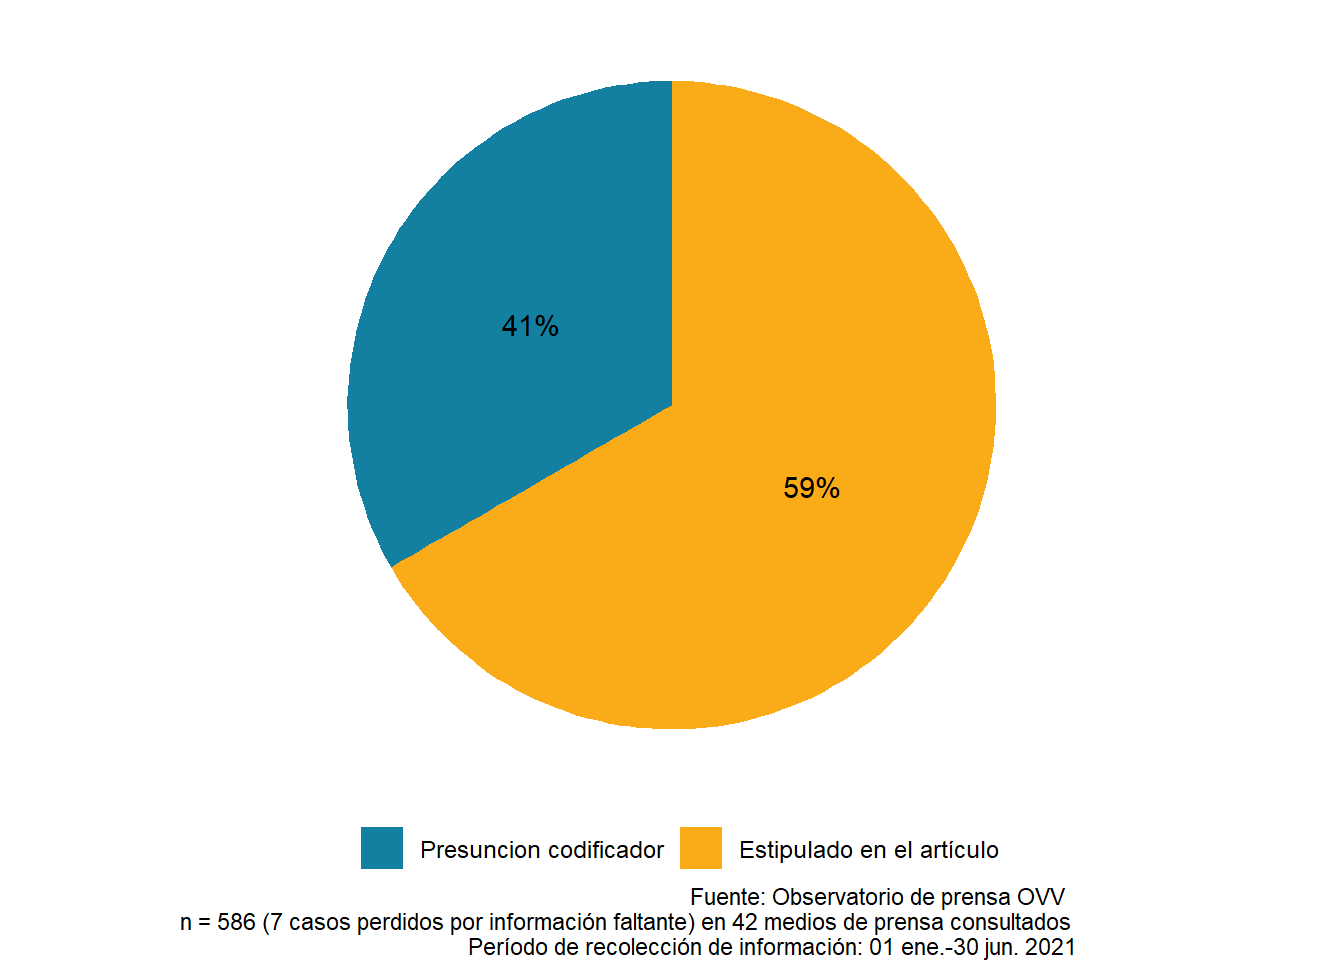
\includegraphics{bookdown-demo_files/figure-latex/sucesoshipresmotivacionhipiegraf-1.pdf}
\caption{\label{fig:sucesoshipresmotivacionhipiegraf}Proporción de sucesos de homicidio intencional discriminados según si la motivación corresponde a la presunción del codificador o el artículo de prensa claramente lo establece.}
\end{figure}

\hypertarget{vuxedctimas-de-otros-delitos}{%
\chapter{Víctimas de otros delitos}\label{vuxedctimas-de-otros-delitos}}

\hypertarget{edad-y-sexo-de-la-vuxedctima-2}{%
\section{Edad y sexo de la víctima}\label{edad-y-sexo-de-la-vuxedctima-2}}



\begin{figure}
\centering
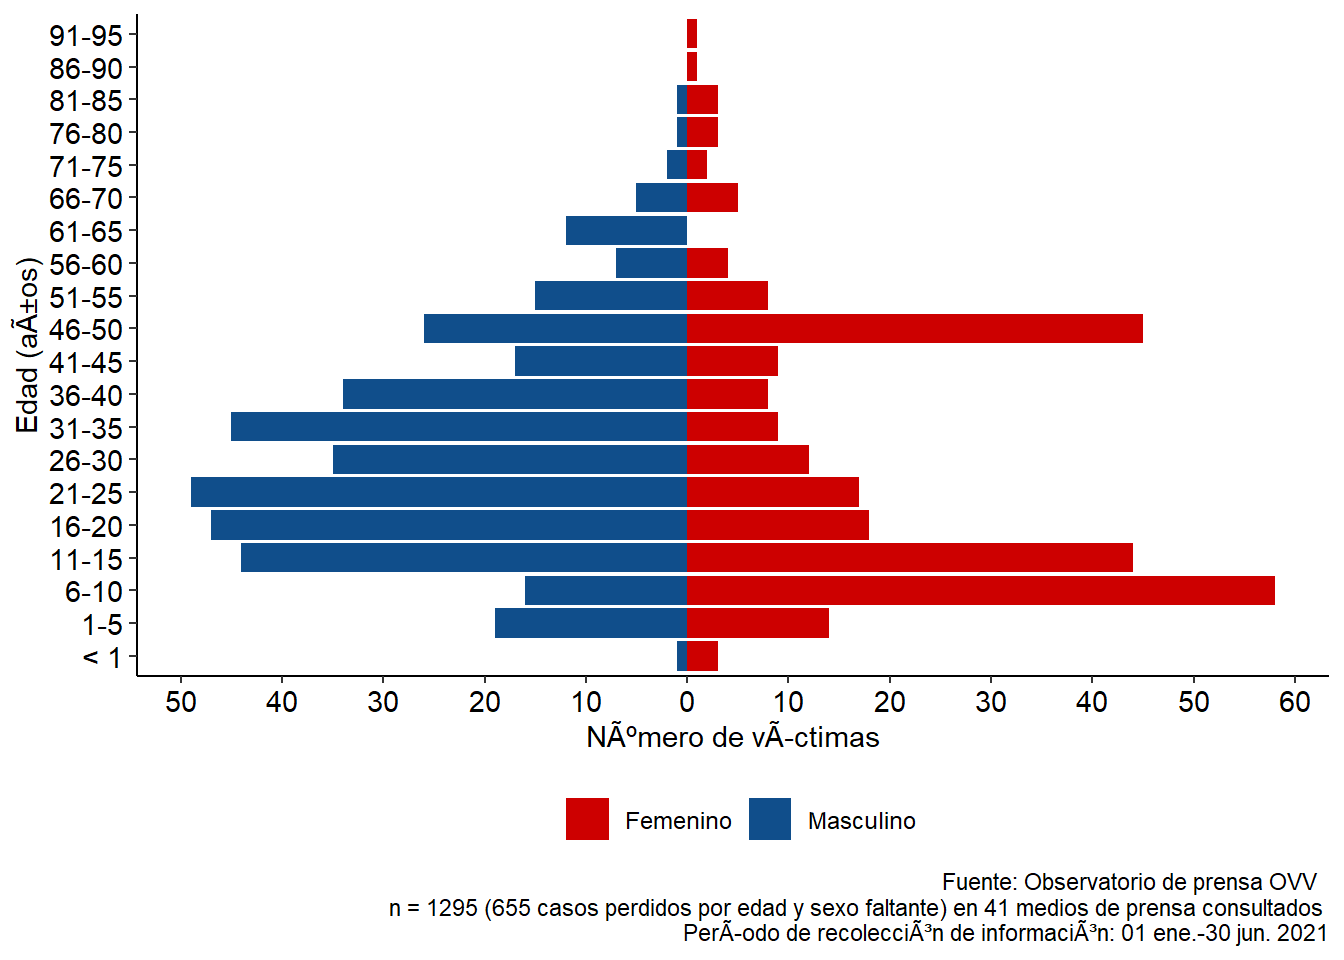
\includegraphics{bookdown-demo_files/figure-latex/victimasodeledadsexopirgraf-1.pdf}
\caption{\label{fig:victimasodeledadsexopirgraf}Número víctimas de otros delitos distintos a homicidio intencional discriminados por edad y sexo.}
\end{figure}

\hypertarget{estado-conyugal-de-la-vuxedctima-2}{%
\section{Estado conyugal de la víctima}\label{estado-conyugal-de-la-vuxedctima-2}}



\begin{figure}
\centering
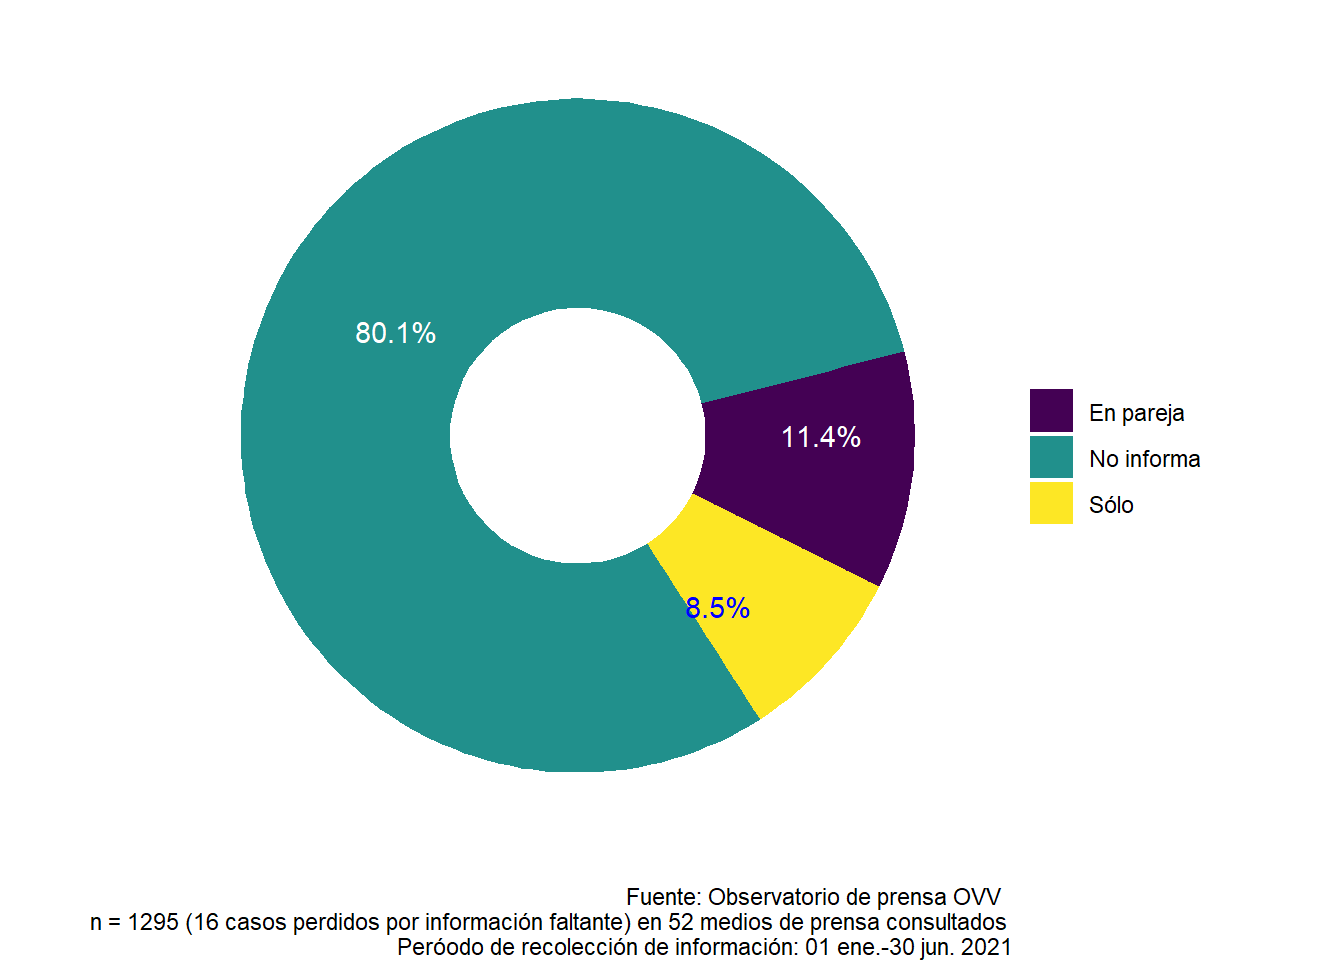
\includegraphics{bookdown-demo_files/figure-latex/victimasodelconyugal-1.pdf}
\caption{\label{fig:victimasodelconyugal}Estado conyugal de víctimas por otros delitos distintos a homicidio intencional.}
\end{figure}

\hypertarget{polivictimizado-1}{%
\section{Polivictimizado}\label{polivictimizado-1}}



\begin{figure}
\centering
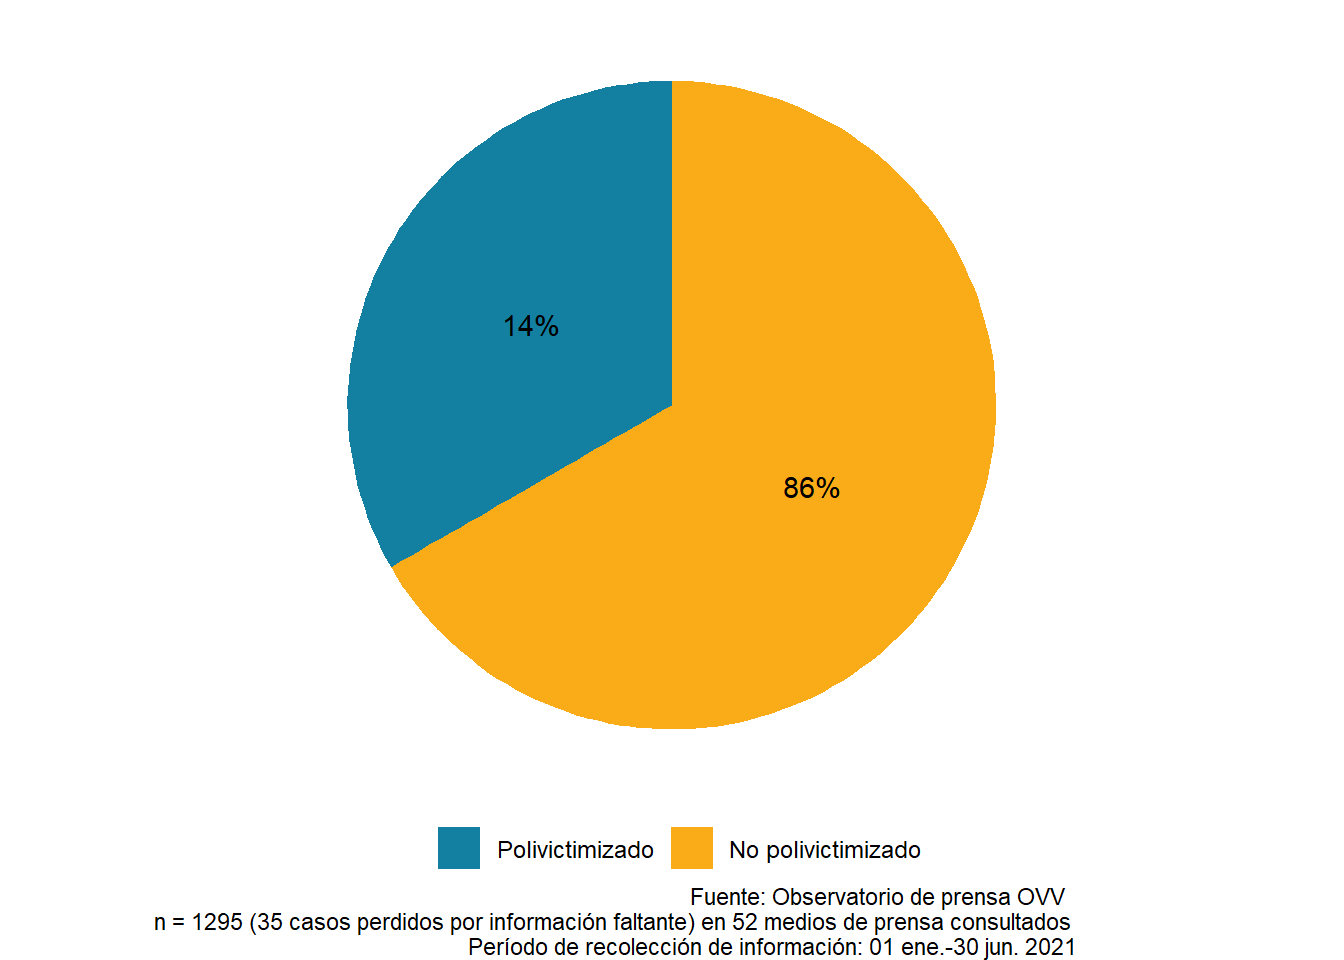
\includegraphics{bookdown-demo_files/figure-latex/victimasodelpoligraf-1.pdf}
\caption{\label{fig:victimasodelpoligraf}Número de víctimas por otros delitos distintos a homicidio intencional discriminados según condición de polivictimización.}
\end{figure}

\hypertarget{condiciuxf3n-de-la-vuxedctima-2}{%
\section{Condición de la víctima}\label{condiciuxf3n-de-la-vuxedctima-2}}



\begin{figure}
\centering
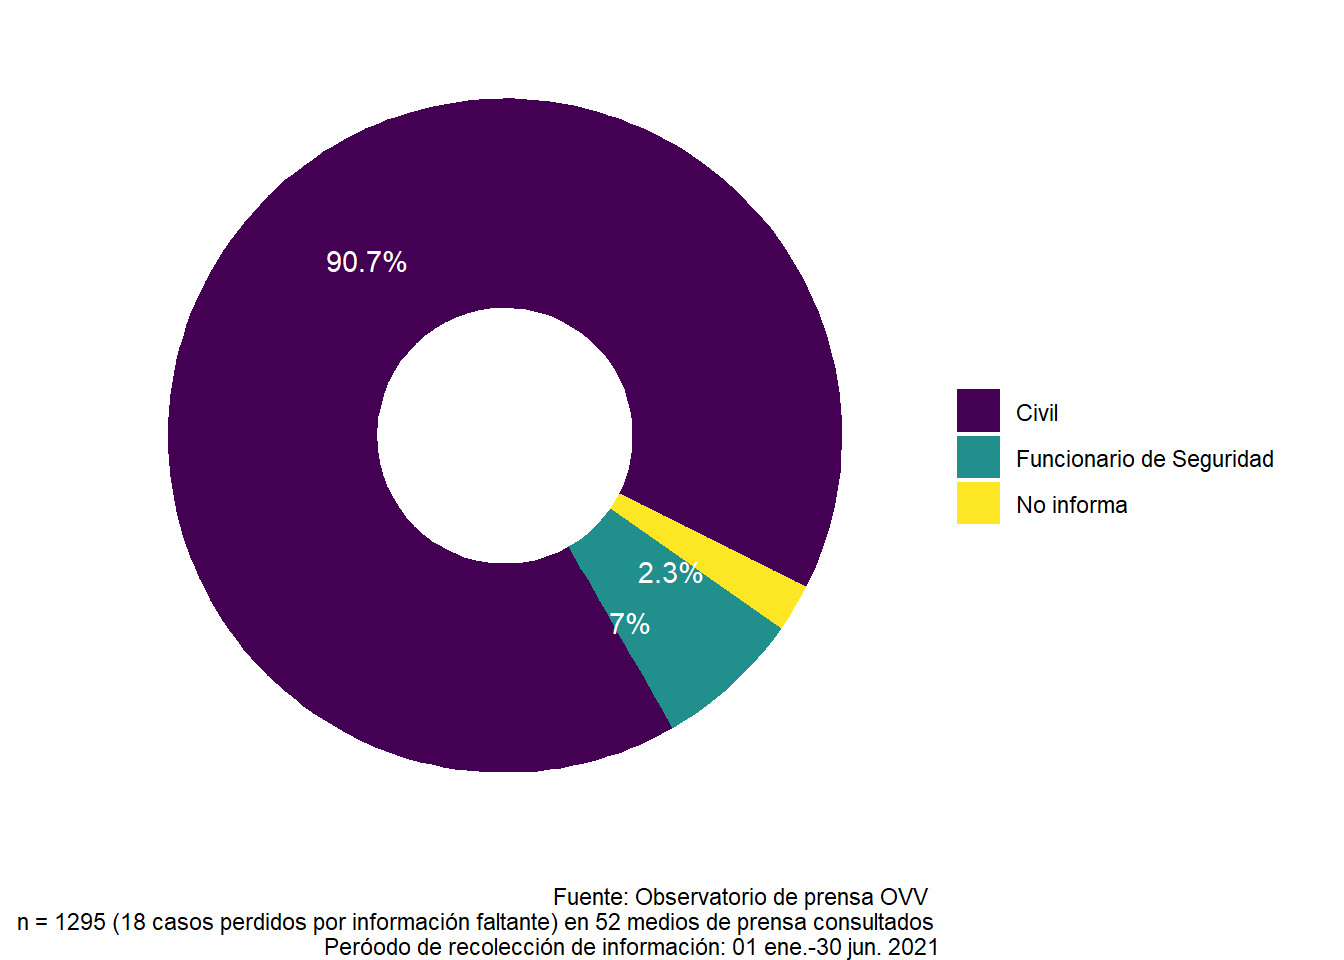
\includegraphics{bookdown-demo_files/figure-latex/victimasodelcondicion-1.pdf}
\caption{\label{fig:victimasodelcondicion}Proporción de víctimas de otros delitos distintos a homicidio intencional discriminadas según su condición de civiles o funcionarios de seguridad.}
\end{figure}

\hypertarget{la-vuxedctima-era-delincuente-2}{%
\section{¿La víctima era delincuente?}\label{la-vuxedctima-era-delincuente-2}}



\begin{figure}
\centering
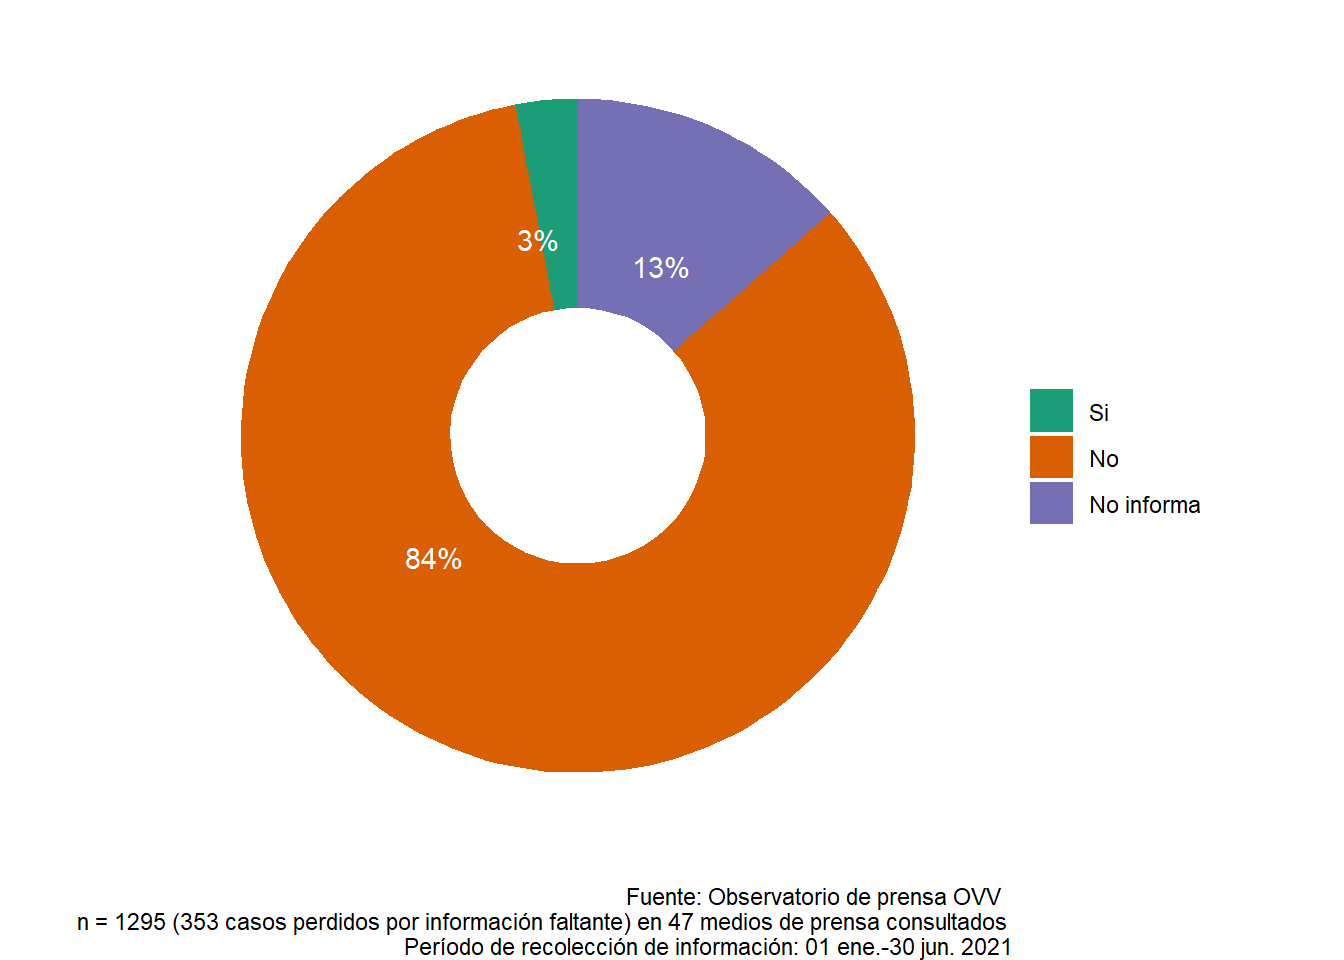
\includegraphics{bookdown-demo_files/figure-latex/victimasodelvictideligraf-1.pdf}
\caption{\label{fig:victimasodelvictideligraf}Número de víctimas por otros delitos distintos a homicidio intencional discriminados según condición de la víctima de ser o no delincuentes.}
\end{figure}

\hypertarget{actividad-de-la-vuxedctima-2}{%
\section{Actividad de la víctima}\label{actividad-de-la-vuxedctima-2}}



\begin{figure}
\centering
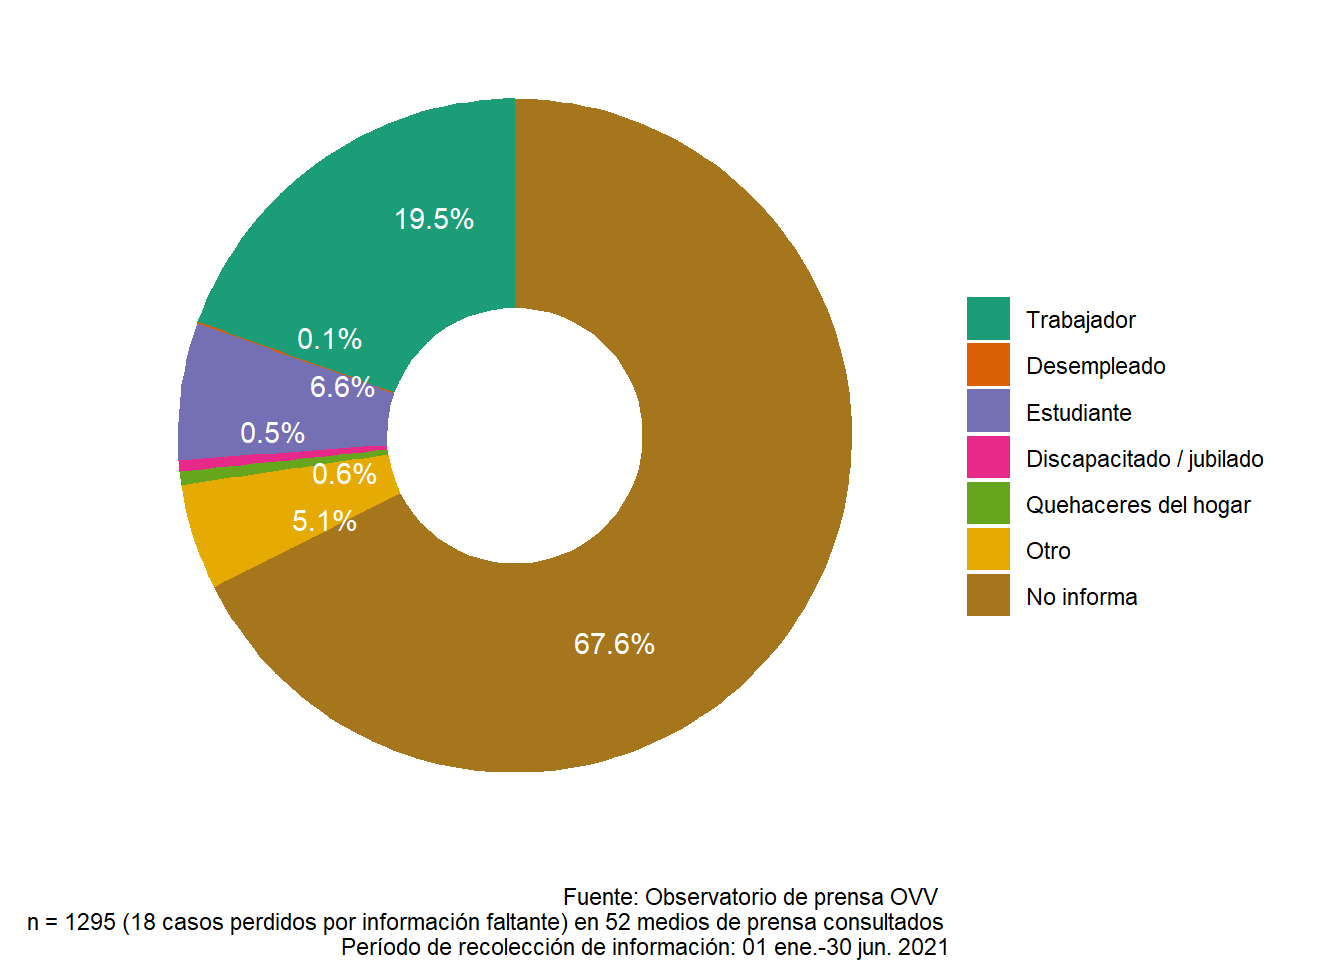
\includegraphics{bookdown-demo_files/figure-latex/victimasodelactividadgraf-1.pdf}
\caption{\label{fig:victimasodelactividadgraf}Número de víctimas por delitos distintos a homicidio intencional discriminados según su actividad.}
\end{figure}



\begin{table}[left]

\caption{\label{tab:victimasodelactividadtable}Número y proporción de víctimas por delitos distintos a homicidio intencional discriminados por su actividad. Período de recolección de información: 01 ene.-30 jun. 2021; n=1295 (18 casos perdidos por información faltante) en 52 medios de prensa consultados.}
\centering
\begin{tabular}[t]{lcr}
\toprule
Ocupación & Víctimas & Porcentaje\\
\midrule
No informa & 297 & 45.6\%\\
No aplica & 181 & 27.8\%\\
Trabajadores servicios & 43 & 6.6\%\\
Agricultores & 40 & 6.1\%\\
Protección & 23 & 3.5\%\\
\addlinespace
Trab. no calificados & 23 & 3.5\%\\
Profesionales & 10 & 1.5\%\\
Técnicos & 9 & 1.4\%\\
Fuerzas armadas & 8 & 1.2\%\\
Artes mecánicas & 7 & 1.1\%\\
\addlinespace
Conductores & 6 & 0.9\%\\
Ejecutivos & 3 & 0.5\%\\
Oficina & 1 & 0.2\%\\
Operadores máquinas & 1 & 0.2\%\\
\bottomrule
\end{tabular}
\end{table}

\hypertarget{ocupaciuxf3n-de-la-vuxedctima-2}{%
\section{Ocupación de la víctima}\label{ocupaciuxf3n-de-la-vuxedctima-2}}



\begin{figure}
\centering
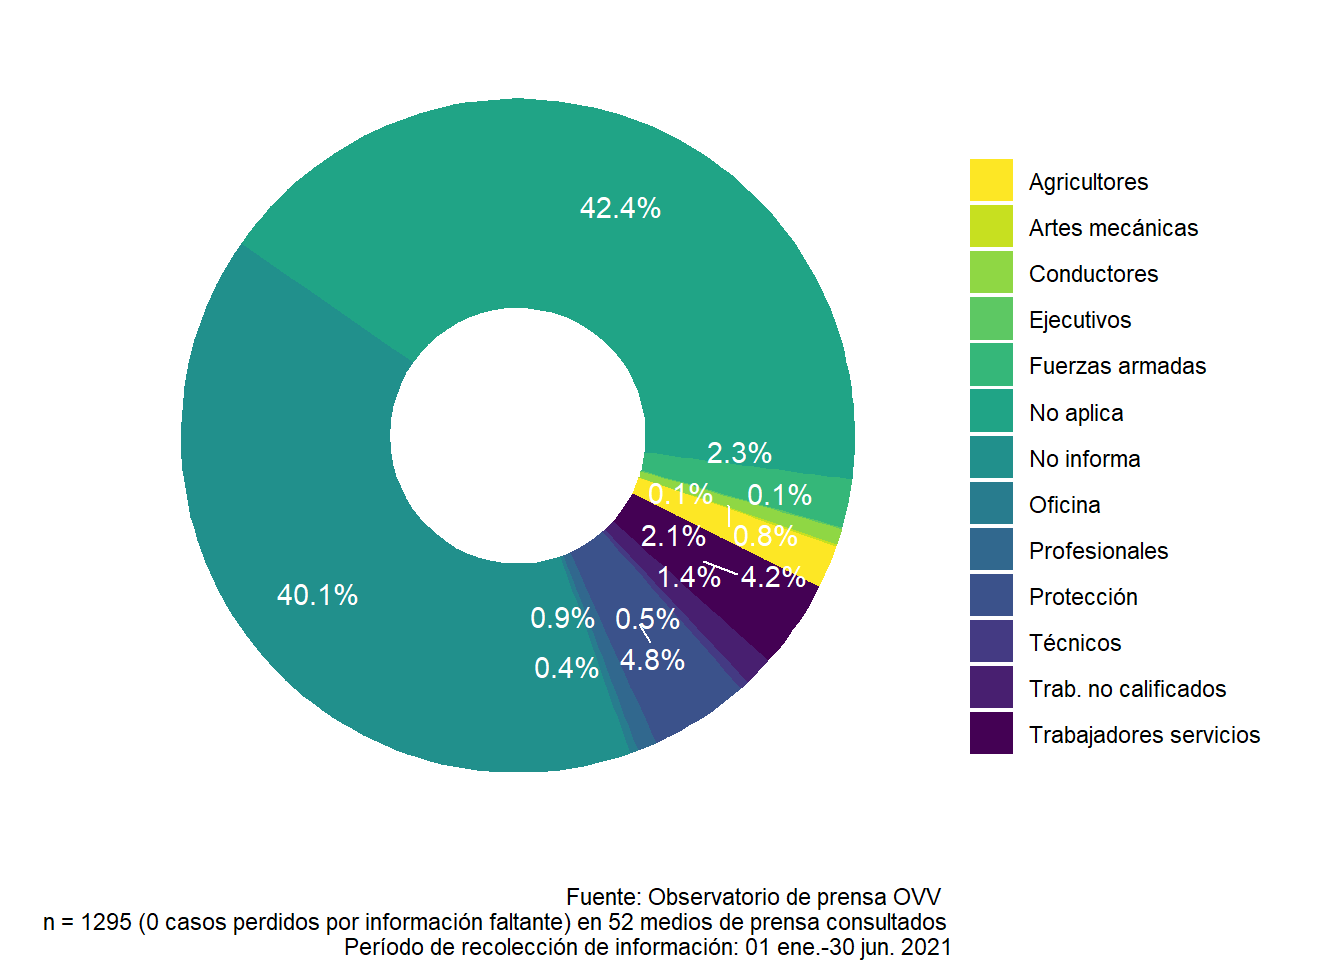
\includegraphics{bookdown-demo_files/figure-latex/victimasodelocupaciongraf-1.pdf}
\caption{\label{fig:victimasodelocupaciongraf}Número de víctimas por otros delitos distintos a homicidio intencional discriminados según su ocupación.}
\end{figure}



\begin{table}[left]

\caption{\label{tab:victimasodelocupaciontable}Número y proporción de víctimas por otros delitos distintos a homicidio intencional discriminados por su ocupación. Período de recolección de información: 01 ene.-30 jun. 2021; n=1295 (0 casos perdidos por información faltante) en 52 medios de prensa consultados.}
\centering
\begin{tabular}[t]{lcr}
\toprule
Ocupación & Víctimas & Porcentaje\\
\midrule
No aplica & 549 & 42.4\%\\
No informa & 519 & 40.1\%\\
Protección & 62 & 4.8\%\\
Trabajadores servicios & 55 & 4.2\%\\
Fuerzas armadas & 30 & 2.3\%\\
\addlinespace
Agricultores & 27 & 2.1\%\\
Trab. no calificados & 18 & 1.4\%\\
Profesionales & 12 & 0.9\%\\
Conductores & 10 & 0.8\%\\
Técnicos & 6 & 0.5\%\\
\addlinespace
Oficina & 5 & 0.4\%\\
Artes mecánicas & 1 & 0.1\%\\
Ejecutivos & 1 & 0.1\%\\
\bottomrule
\end{tabular}
\end{table}

\hypertarget{eventos-otros-delitos}{%
\chapter{Eventos otros delitos}\label{eventos-otros-delitos}}

\hypertarget{proporciones-generales}{%
\section{Proporciones generales}\label{proporciones-generales}}



\begin{figure}
\centering
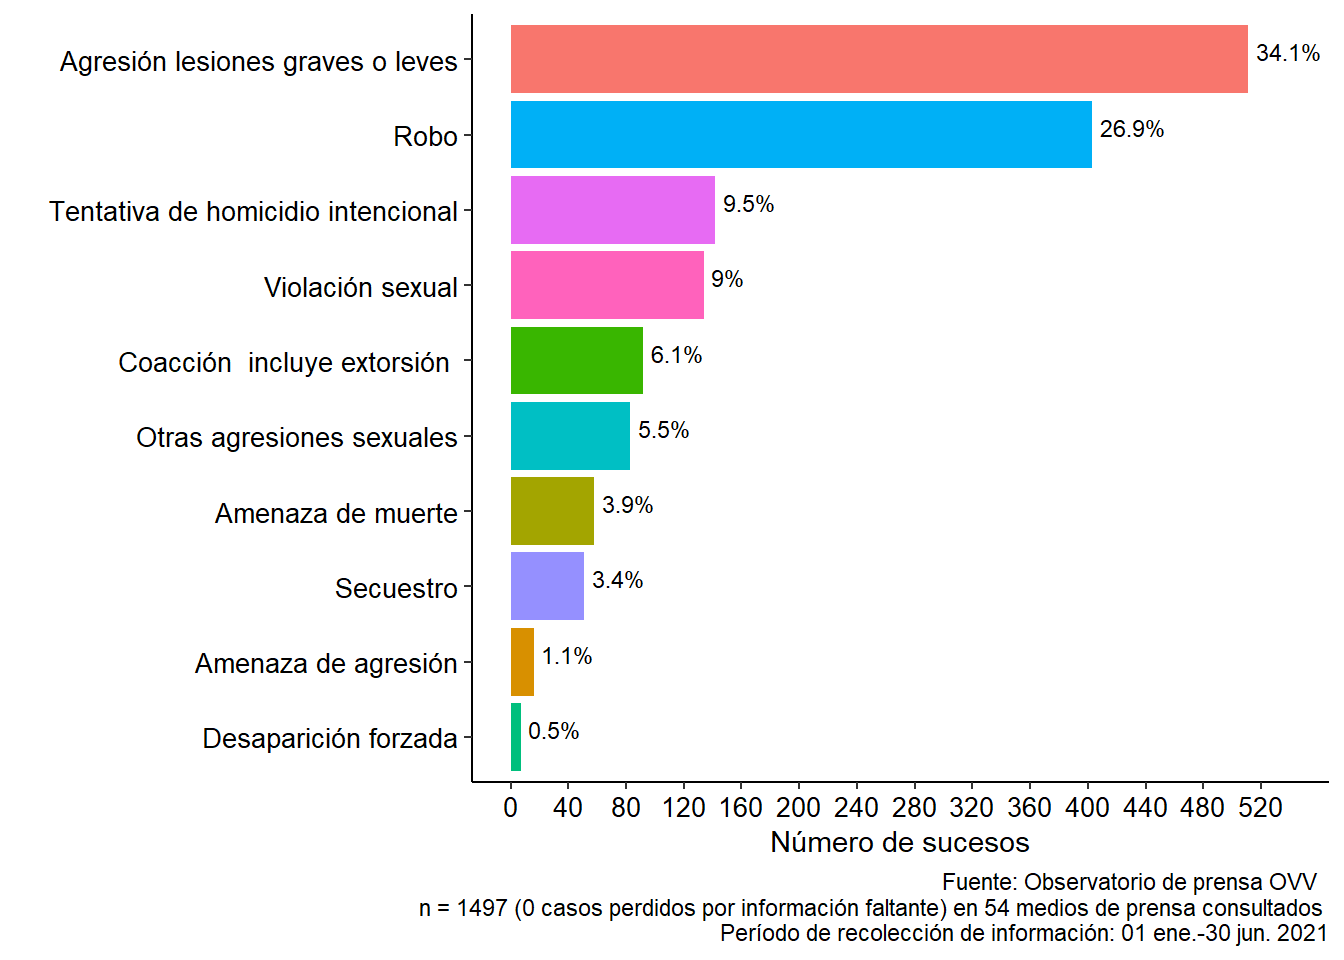
\includegraphics{bookdown-demo_files/figure-latex/sucesosotrosdelbarragraf-1.pdf}
\caption{\label{fig:sucesosotrosdelbarragraf}Proporción de sucesos de otros delitos distintos a homicidio intencional discriminados según el tipo de delito.}
\end{figure}

\hypertarget{nuxfamero-de-vuxedctimas}{%
\section{Número de víctimas}\label{nuxfamero-de-vuxedctimas}}



\begin{figure}
\centering
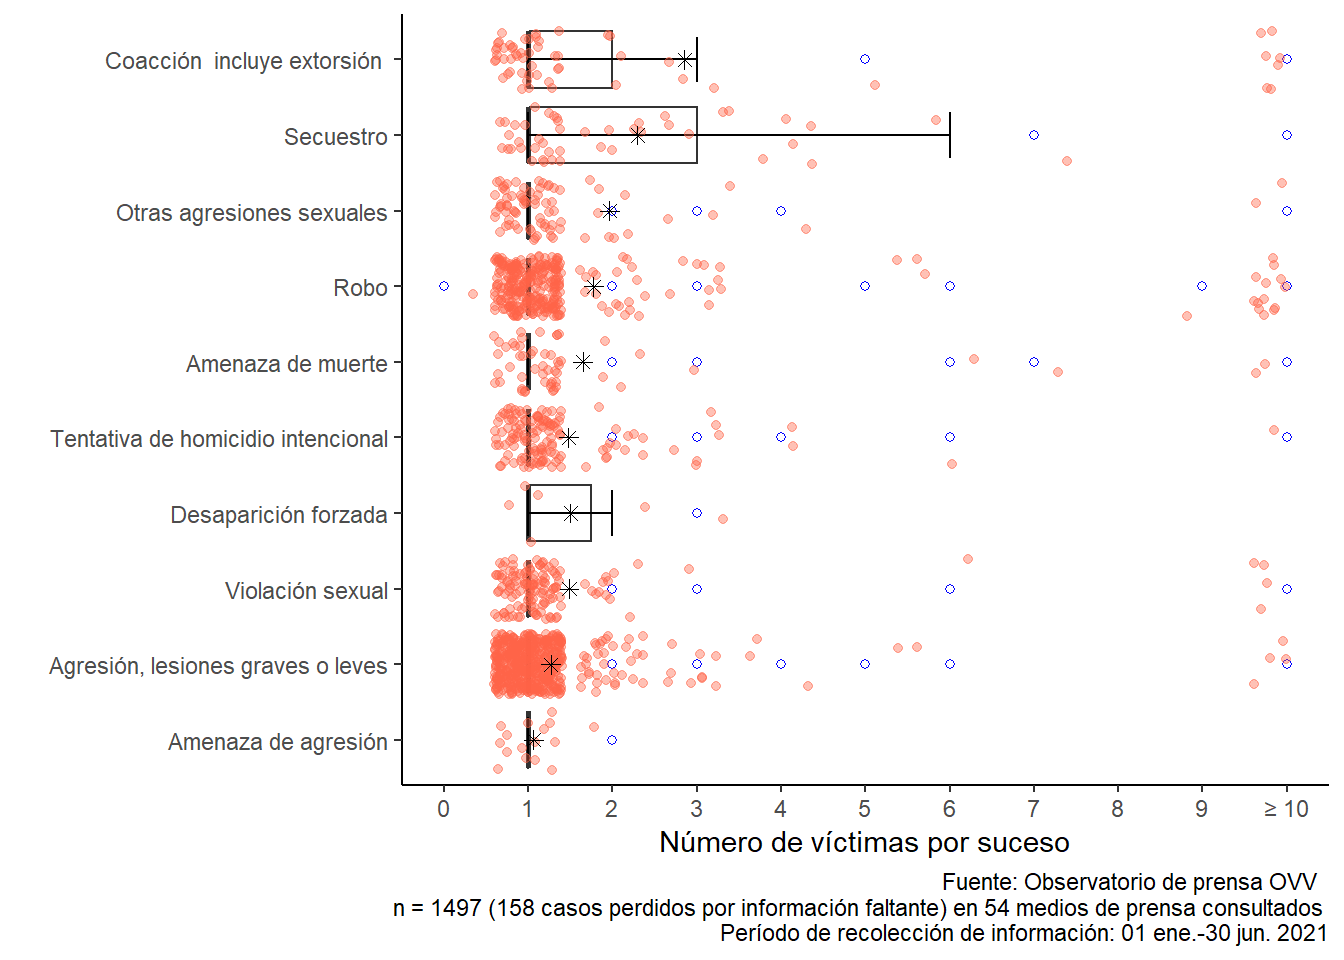
\includegraphics{bookdown-demo_files/figure-latex/sucesosotrosdelnumvictimasboxplotgraf-1.pdf}
\caption{\label{fig:sucesosotrosdelnumvictimasboxplotgraf}Distribución del número de víctimas por sucesos de otros delitos distintos a homicidio intencional discriminados según el tipo de delito.}
\end{figure}

\hypertarget{nuxfamero-de-vuxedctimarios}{%
\section{Número de víctimarios}\label{nuxfamero-de-vuxedctimarios}}



\begin{figure}
\centering
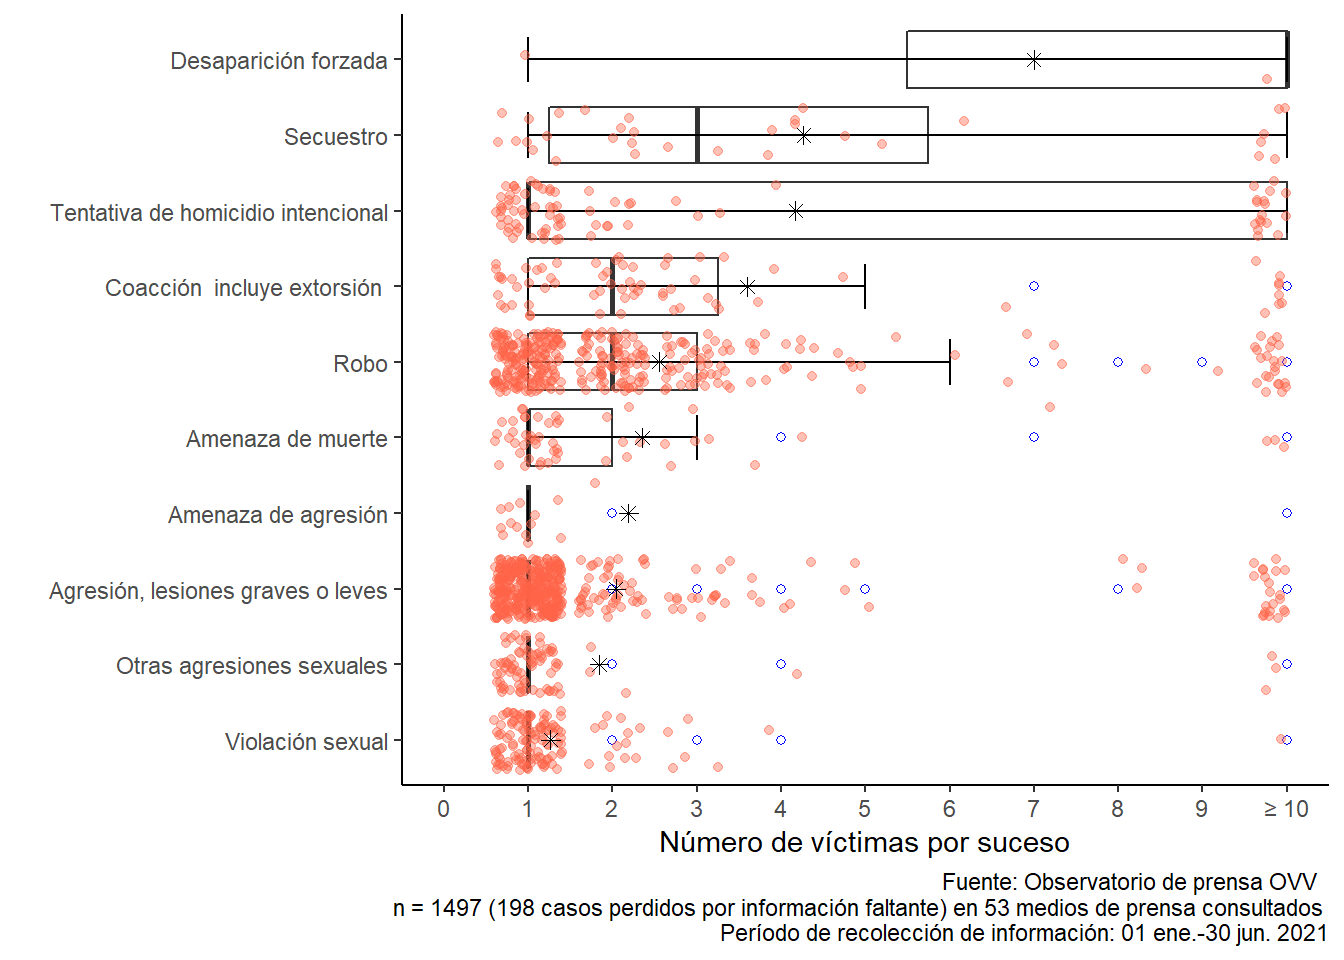
\includegraphics{bookdown-demo_files/figure-latex/sucesosotrosdelnumvictimariosboxplotgraf-1.pdf}
\caption{\label{fig:sucesosotrosdelnumvictimariosboxplotgraf}Distribución del número de víctimarios por sucesos de otros delitos distintos a homicidio intencional discriminados según el tipo de delito.}
\end{figure}

\hypertarget{duxeda-de-ocurrencia-1}{%
\section{Día de ocurrencia}\label{duxeda-de-ocurrencia-1}}



\begin{figure}
\centering
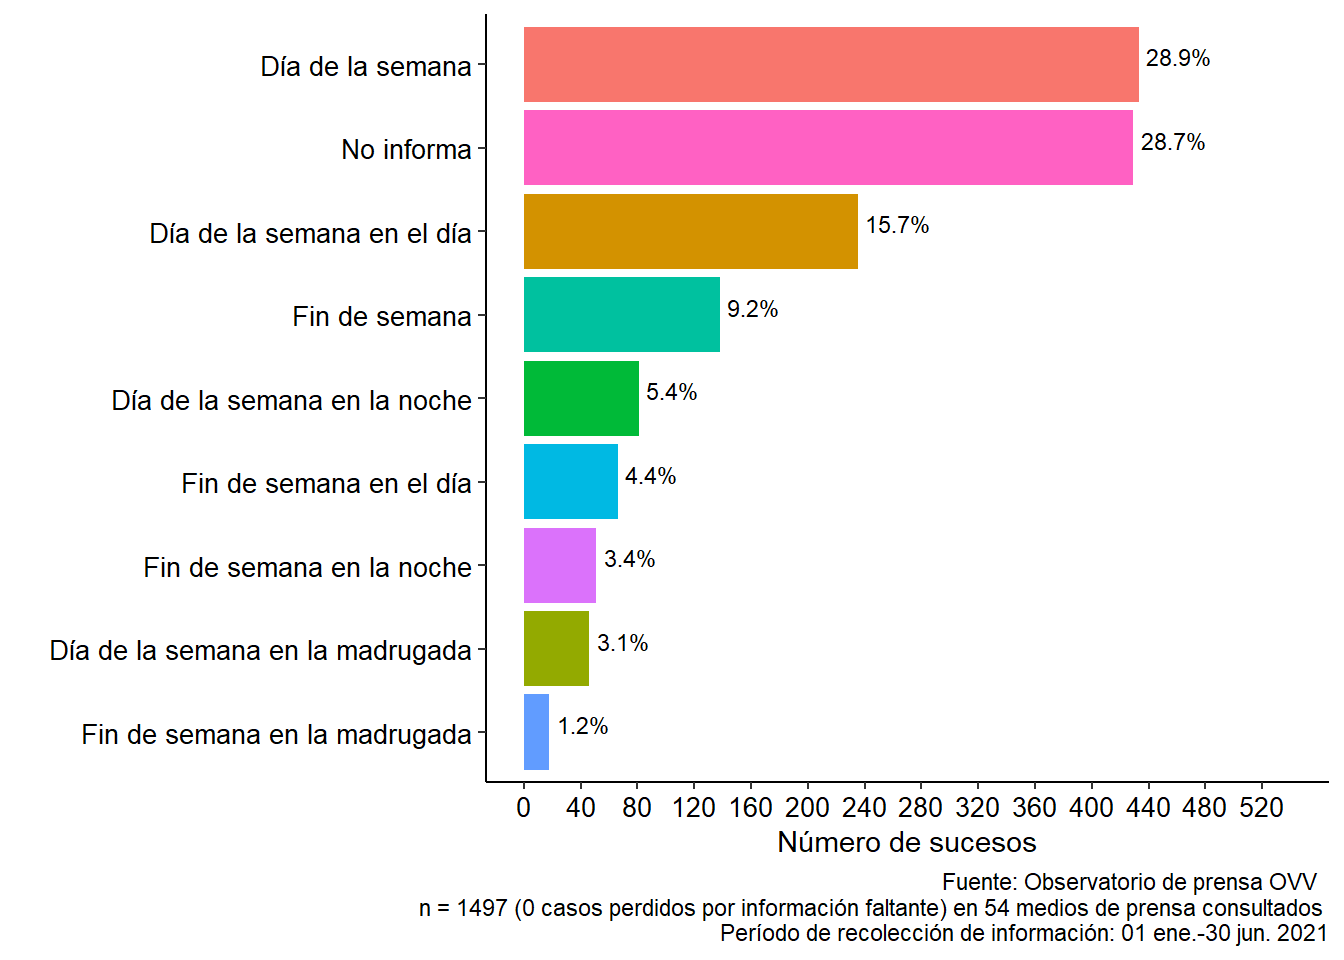
\includegraphics{bookdown-demo_files/figure-latex/sucodelcuanbargraf-1.pdf}
\caption{\label{fig:sucodelcuanbargraf}Distribución del número de víctimarios por sucesos de otros delitos distintos a homicidio intencional discriminados según cuando ocurrió el delito.}
\end{figure}

\hypertarget{sitio-de-ocurrencia-1}{%
\section{Sitio de ocurrencia}\label{sitio-de-ocurrencia-1}}



\begin{figure}
\centering
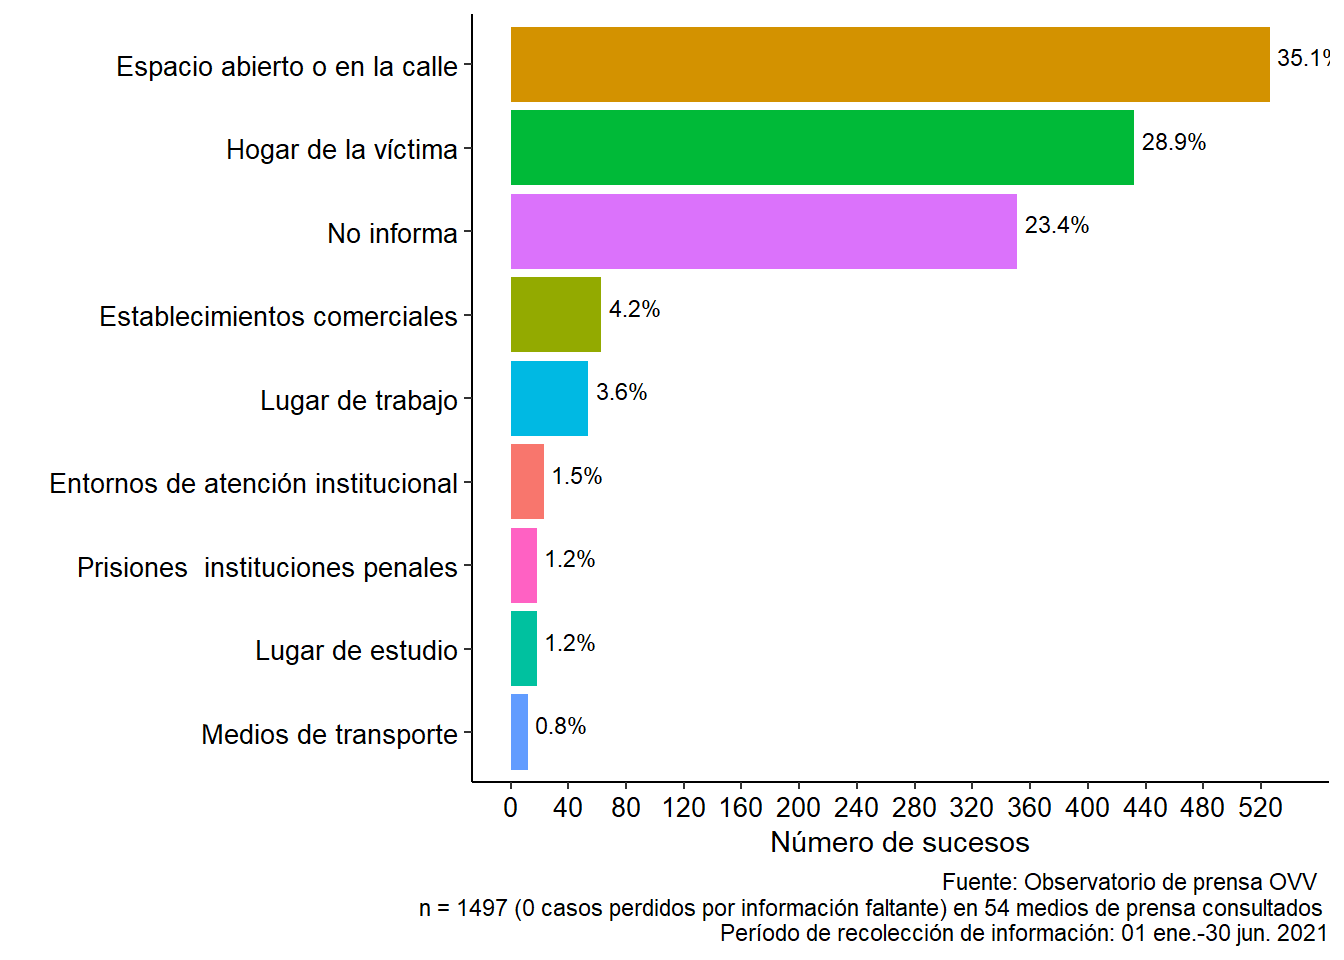
\includegraphics{bookdown-demo_files/figure-latex/sucesosotrosdeldondebarrasgraf-1.pdf}
\caption{\label{fig:sucesosotrosdeldondebarrasgraf}Distribución del número de sucesos de otros delitos distintos a homicidio intencional discriminados según donde fueron cometidos.}
\end{figure}

\hypertarget{cercanuxeda-a-la-vivienda-de-la-vuxedctima}{%
\section{Cercanía a la vivienda de la víctima}\label{cercanuxeda-a-la-vivienda-de-la-vuxedctima}}



\begin{figure}
\centering
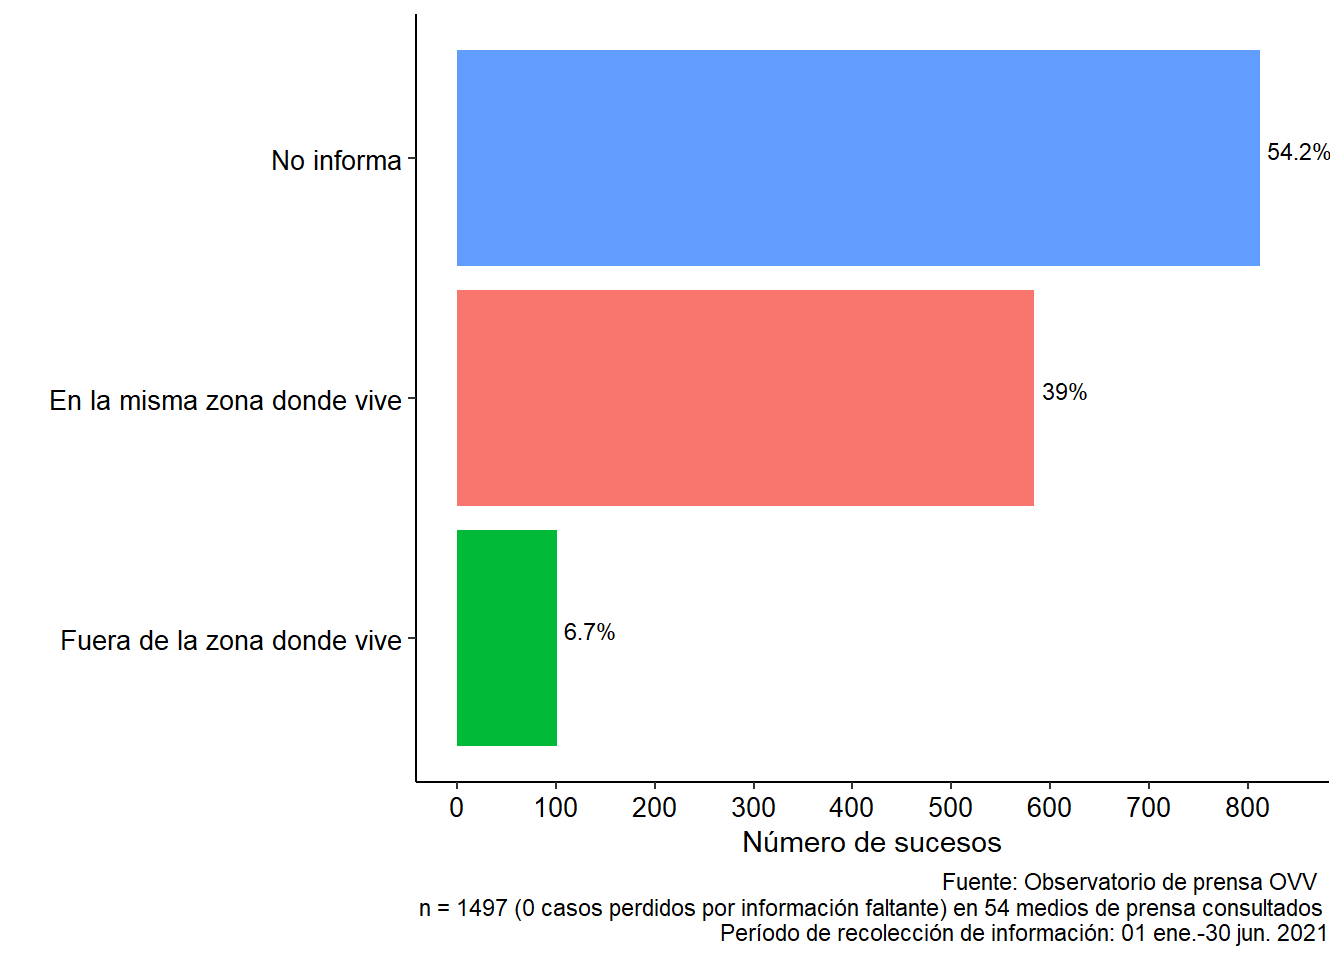
\includegraphics{bookdown-demo_files/figure-latex/suodelcercabargraf-1.pdf}
\caption{\label{fig:suodelcercabargraf}Distribución del número de sucesos de otros delitos distintos a homicidio intencional discriminados según cercanía a la vivienda de la víctima.}
\end{figure}

\hypertarget{tipo-de-arma-1}{%
\section{Tipo de arma}\label{tipo-de-arma-1}}



\begin{figure}
\centering
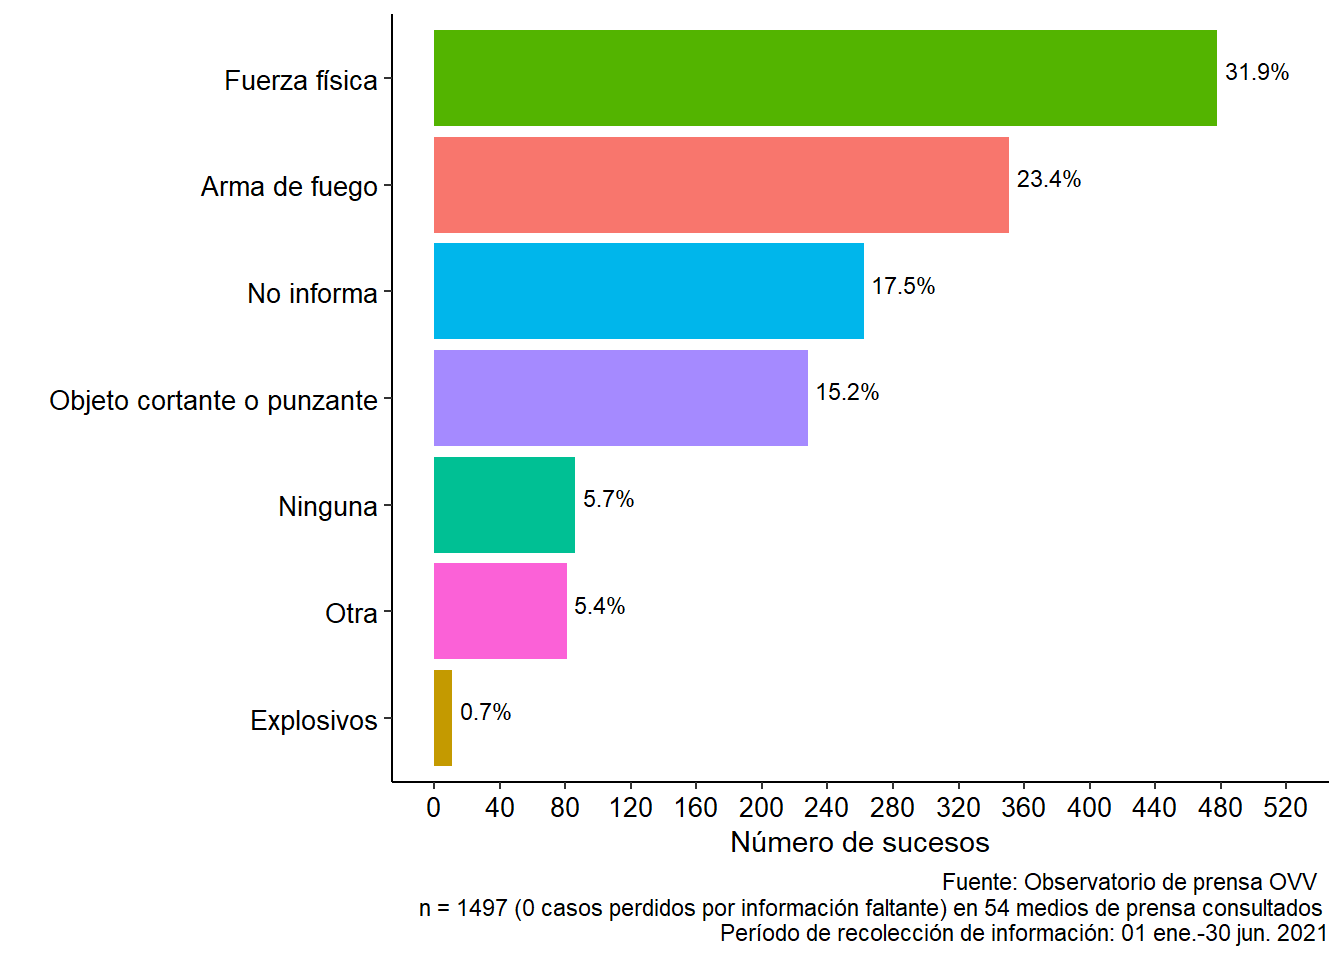
\includegraphics{bookdown-demo_files/figure-latex/suodeltarmabargraf-1.pdf}
\caption{\label{fig:suodeltarmabargraf}Distribución del número de sucesos de otros delitos distintos a homicidio intencional discriminados según el tipo de arma utilizada.}
\end{figure}

\hypertarget{relaciuxf3n-con-victimario}{%
\section{Relación con victimario}\label{relaciuxf3n-con-victimario}}



\begin{figure}
\centering
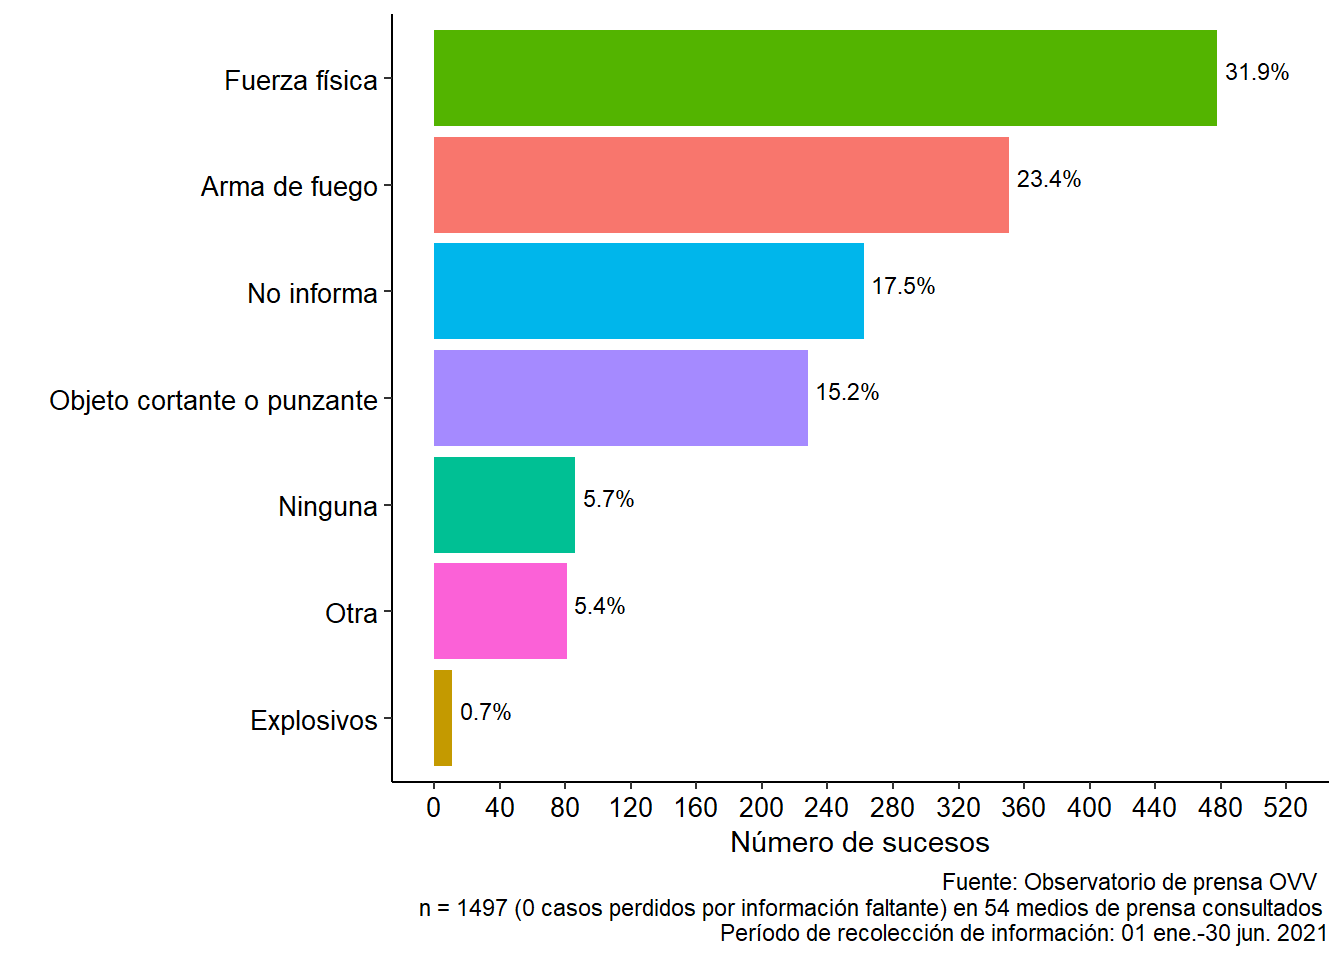
\includegraphics{bookdown-demo_files/figure-latex/suodelqvictimariobargraf-1.pdf}
\caption{\label{fig:suodelqvictimariobargraf}Distribución del número de sucesos de otros delitos distintos a homicidio intencional discriminados según el tipo de relación con el victimario.}
\end{figure}

\hypertarget{victimario-conocido-o-familiar}{%
\section{¿Victimario conocido o familiar?}\label{victimario-conocido-o-familiar}}



\begin{figure}
\centering
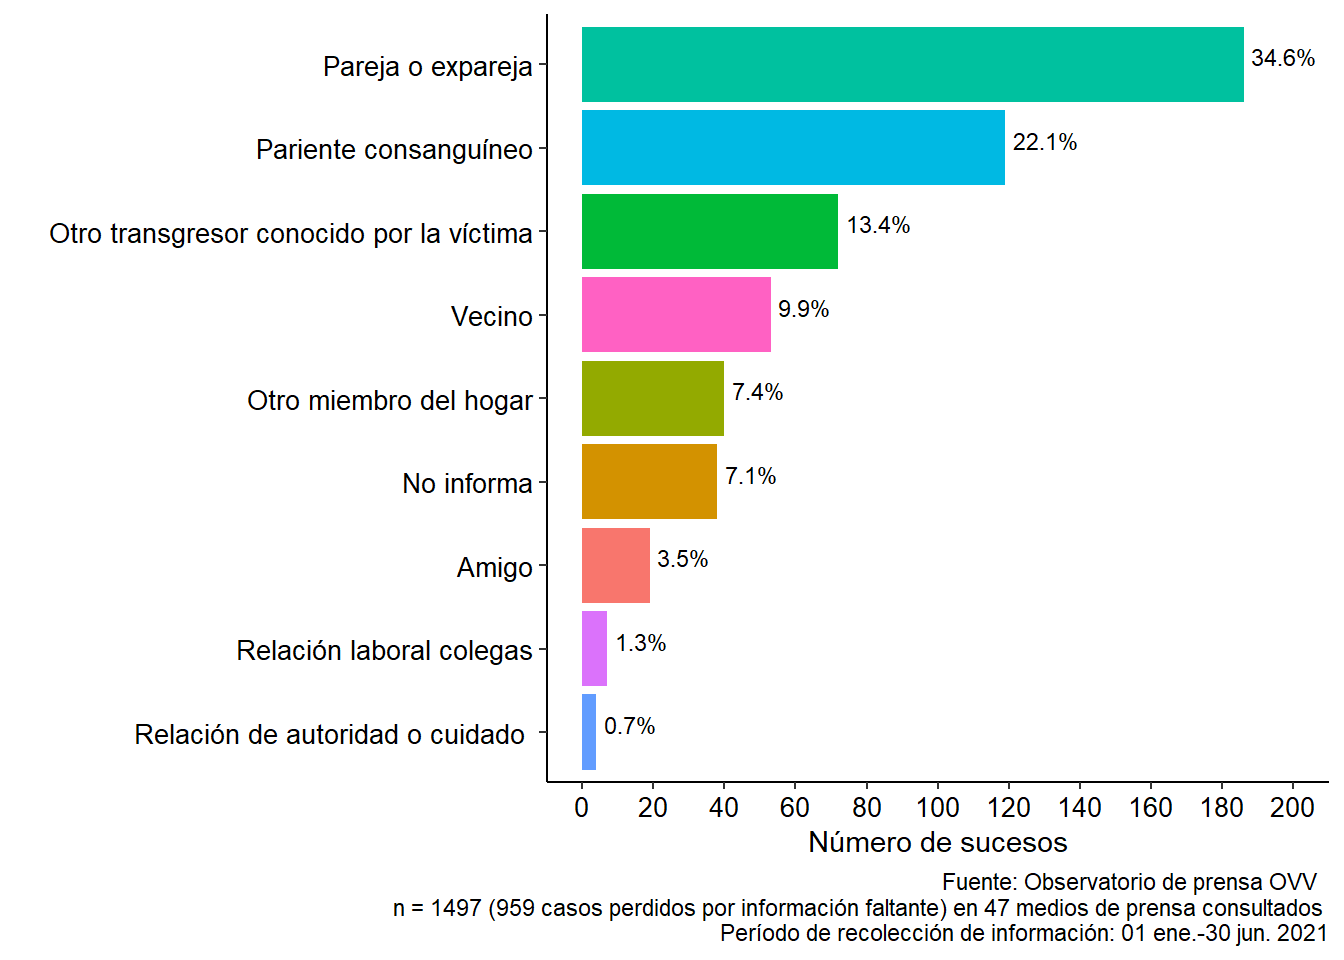
\includegraphics{bookdown-demo_files/figure-latex/suodelcvictimariobargraf-1.pdf}
\caption{\label{fig:suodelcvictimariobargraf}Distribución del número de sucesos de otros delitos distintos a homicidio intencional discriminados según el tipo de relación con el victimario.}
\end{figure}

\hypertarget{el-victimario-es-funcionario}{%
\section{¿El victimario es funcionario?}\label{el-victimario-es-funcionario}}



\begin{figure}
\centering
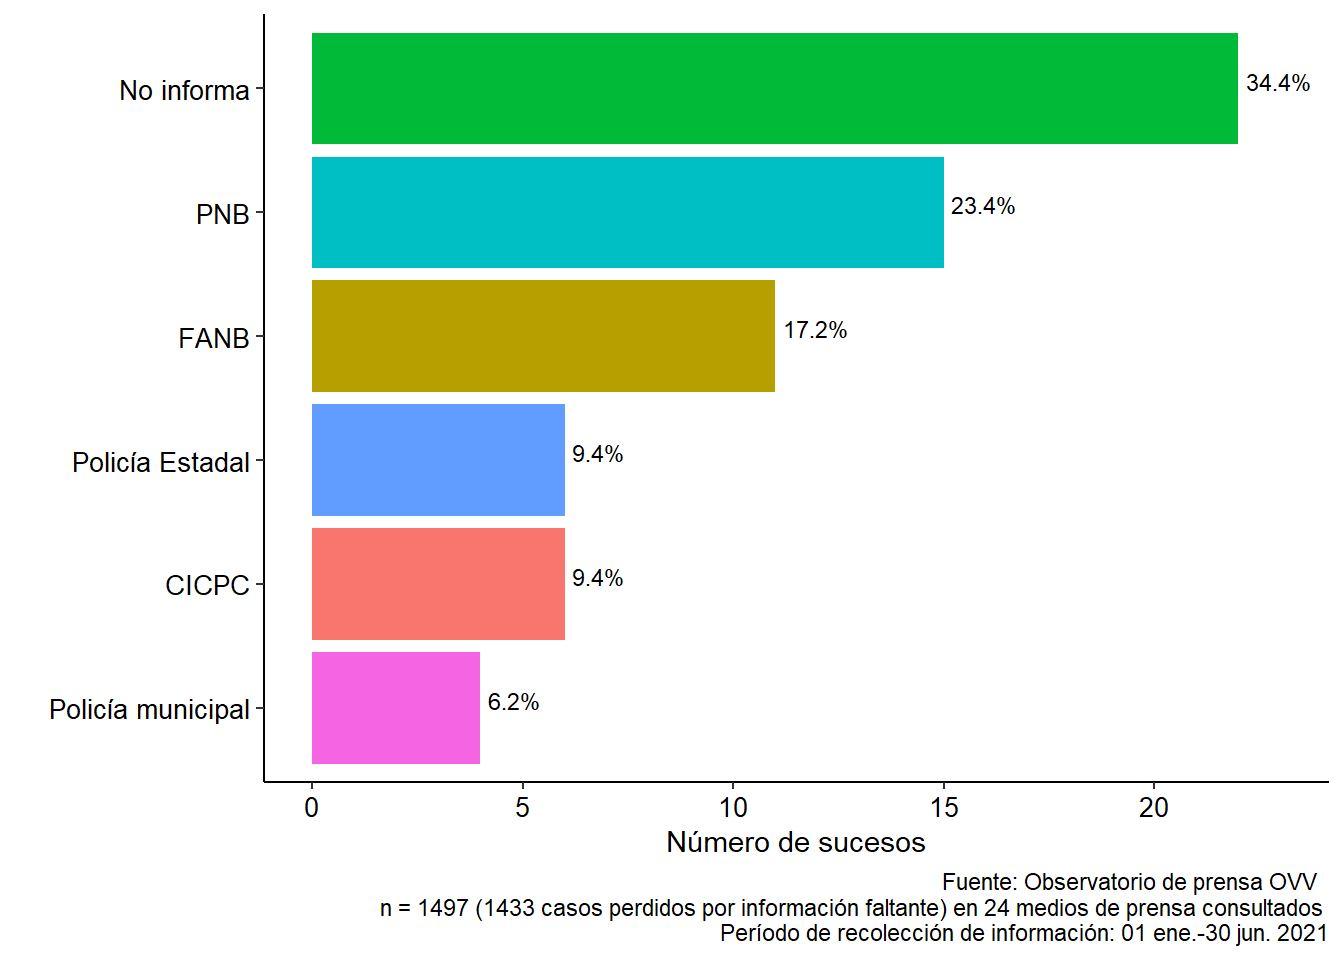
\includegraphics{bookdown-demo_files/figure-latex/suodelosvictimariobargraf-1.pdf}
\caption{\label{fig:suodelosvictimariobargraf}Distribución del número de sucesos de otros delitos distintos a homicidio intencional discriminados según el organismo de seguridad del victimario en el caso de que este fuese funcionario.}
\end{figure}

\hypertarget{con-que-se-relaciona-el-suceso}{%
\section{¿Con que se relaciona el suceso?}\label{con-que-se-relaciona-el-suceso}}



\begin{figure}
\centering
\includegraphics{bookdown-demo_files/figure-latex/suodelcquebargraf-1.pdf}
\caption{\label{fig:suodelcquebargraf}Distribución del número de sucesos de otros delitos distintos a homicidio intencional discriminados según el contexto del suceso.}
\end{figure}



\begin{figure}
\centering
\includegraphics{bookdown-demo_files/figure-latex/suodelprescquebargraf-1.pdf}
\caption{\label{fig:suodelprescquebargraf}Distribución del número de sucesos de otros delitos distintos a homicidio intencional discriminados según si el contexto del suceso es presunción del codificador o estipulado en el artículo de prensa.}
\end{figure}

\hypertarget{motivaciuxf3n-del-suceso}{%
\section{Motivación del suceso}\label{motivaciuxf3n-del-suceso}}



\begin{figure}
\centering
\includegraphics{bookdown-demo_files/figure-latex/suodelmotivacionbar-1.pdf}
\caption{\label{fig:suodelmotivacionbar}Distribución del número de sucesos de otros delitos distintos a homicidio intencional discriminados según la motivacion del delito.}
\end{figure}



\begin{figure}
\centering
\includegraphics{bookdown-demo_files/figure-latex/suodelpresmotivacionpiegraf-1.pdf}
\caption{\label{fig:suodelpresmotivacionpiegraf}Distribución del número de sucesos de otros delitos distintos a homicidio intencional discriminados según si la motivación del suceso es presunción del codificador o estipulado en el artículo de prensa.}
\end{figure}

  \bibliography{book.bib,packages.bib}

\end{document}
